% ******************************* PhD Thesis Template **************************
% Please have a look at the README.md file for info on how to use the template

% **************************** Formatting & Metadata ***************************

\documentclass[a4paper,12pt,times,print,custombib,chapter]{_Meta/thesis}
% See README.md for option details

\input{_Meta/preamble} %Contains packages and user-defined commands and settings
%
%% ************************ Thesis Information & Meta-data **********************
%
% ************************ Thesis Information & Meta-data **********************
%% The title of the thesis
\title{Characterising antibody immunity and ageing in a short-lived teleost}

%% Subtitle (Optional)
%\subtitle{}
%\submissiontext

%% The full name of the author
\author{William John Bradshaw}

%% Department (eg. Department of Engineering, Maths, Physics)
\dept{aus Hastings} %! Really?

%% University and Crest
%\university{University of Cologne, Germany}
% Crest minimum should be 30mm.
\crest{\includegraphics[width=0.5\textwidth]{_Meta/Logos/UoC_Crest}}

%% Use this crest, if you are using the college crest
%% Crest long miminum should be 65mm
%\crest{\includegraphics[width=0.45\textwidth]{University_Crest_Long}}

%% College shield [optional] 
% Crest minimum should be 30mm.
%\collegeshield{\includegraphics[width=0.2\textwidth]{CollegeShields/Kings}}


% Supervisor (optional)
% for multiple supervisors, append each supervisor with the \newline command
\supervisor{Dr. Dario Riccardo Valenzano\newline Prof. Dr. Andreas Beyer}

%% Supervisor line width: required to align supervisors
\supervisorlinewidth{\textwidth}


%% You can redefine the submission text:
% Default as per the University guidelines:
% ``This dissertation is submitted for the degree of''
%\renewcommand{\submissiontext}{change the default text here if needed}

%% Full title of the Degree
%\degreetitle{Doctor of Philosophy}

%% College affiliation (optional)
%\college{MPI for Biology of Ageing}

%% Submission date
% Default is set as {\monthname[\the\month]\space\the\year}
%\degreedate{September 2014} 

%%% Meta information
%\subject{LaTeX} \keywords{{LaTeX} {PhD Thesis} {Engineering} {University of
%Cambridge}}
 % Thesis title and author information, other metadata

% ***************************** Abstract Separate ******************************
% To printout only the titlepage and the abstract with the PhD title and the
% author name for submission to the Student Registry, use the `abstract' option in
% the document class.

\ifdefineAbstract
 \pagestyle{empty}
 \includeonly{A_Frontmatter/2_abstract-de,A_Frontmatter/3_abstract-en,C_Backmatter/declaration}
\fi

% ***************************** Chapter Mode ***********************************
% The chapter mode allows user to only print particular chapters with references
% Title, Contents, Frontmatter are disabled by default
% Useful option to review a particular chapter or to send it to supervisior.
% To use choose `chapter' option in the document class

\ifdefineChapter
	%\includeonly{B_Chapters/1_Introduction/Introduction}
	%\includeonly{B_Chapters/2_Methods/Methods,C_Appendices/Solutions,C_Appendices/Primers,C_Appendices/Diversity,C_Appendices/Tables}
	%\includeonly{B_Chapters/3_Locus/Locus,C_Appendices/Figures,C_Appendices/Tables}
	%\includeonly{B_Chapters/4_IgSeq/IgSeq,C_Appendices/Diversity}%,C_Appendices/Figures,C_Appendices/Tables}
	\includeonly{C_Appendices/Solutions,C_Appendices/Primers,C_Appendices/Diversity,C_Appendices/Tables}
\fi

\begin{document}
\maketitle

%% ******************************** Front Matter ********************************
%% Dedication, abstracts, acknowledgements etc. - do this last.

\frontmatter
% ******************************* Thesis Dedidcation ********************************

\begin{dedication} 
\doublespacing
\raggedleft
\textit{
\begin{LARGE}
Cre\'{e}r, c'est recombiner.\\
\end{LARGE}
-- Fran\c{c}ois Jacob \citep{hsu2015pathogen}}
\end{dedication}


% ************************** Thesis Abstract *****************************
% Use `abstract' as an option in the document class to print only the titlepage and the abstract.
\begin{zusammenfassung}
\end{zusammenfassung}
% ************************** Thesis Abstract *****************************
% Use `abstract' as an option in the document class to print only the titlepage and the abstract.
\begin{abstract}
\textbf{Motivation:} %Circular RNAs are a special class of RNA forming a covalently closed loop through a process called back-splicing. Not much is known about the function of circRNAs. Only for a few well studied circRNAs, potential functions were shown, these include miRNA sponging, RNA binding protein (RBP) sponging, and regulation of their host gene's transcription. Circular RNAs can be identified in rRNA depleted RNA-Sequencing by detecting chimeric reads, which span a back-splice junction. A variety of circRNA detection tools exists but no tool is able to summarize and characterize the identified circRNAs. To perform accurate downstream analyses after circRNA detection, it is crucial to know the exact exon-intron structure of circRNAs. Recently, two tools were published, which identify alternative splicing within circRNAs. Here, I am presenting \texttt{FUCHS} and \texttt{FUCHS\textit{denovo}} to summarize circRNAs and reconstruct their exon-intron chain based on liner-splice signals of back-splice junction anchored reads.

\textbf{Methods:} %In this study, I compared three state of the art circRNA detection programs. Based on the best tool, I developed a Python-based pipeline called \texttt{FUCHS}: \textbf{FU}ll \textbf{CH}aracterization of circular RNA using RNA-\textbf{S}equencing. This pipeline summarizes circRNAs by their host genes, detects skipped exons, finds double-breakpoint fragments, generates circle-wise coverage profiles, and clusters these profiles. Running \texttt{FUCHS} on a mouse dataset indicated that annotated gene models are not always suited to describe the circRNA's exon-intron structure. Hence, I developed an additional module, \texttt{FUCHS\textit{denovo}}, to reconstruct the exon-intron structure based on linear-splice signals of back-splice junction anchored reads. To demonstrate how \texttt{FUCHS} and \texttt{FUCHS\textit{denovo}} perform, I ran both programs on a dataset of young and old murine hearts and young and old murine livers.

\textbf{Results:} %The comparison of three circRNA detection programs (\texttt{DCC}, \texttt{CIRI}, and \texttt{KNIFE}) indicated \texttt{DCC} as the fastest and most accurate circRNA detection program. Running \texttt{FUCHS} on four mouse samples revealed that heart circRNAs are less diverse but more abundant than liver circRNAs. Considering only annotated exons, the average length of circRNAs was 500 BP. Heart circRNAs were longer than liver circRNAs. From the obtained coverage profiles, I concluded that annotated gene models were not always matching the exon-intron structure of circRNAs. A \textit{de novo} reconstruction of the inner circle structure using \texttt{FUCHS\textit{denovo}} showed a gain of information of 15 \%. Furthermore, \texttt{FUCHS\textit{denovo}} identified alternative splicing in 8 - 10 \% of circRNAs. Performing a differential motif enrichment analysis of the flanking introns of circRNAs with alternative splicing over circRNAs without alternative splicing identified FOXO as a potential transcription factor driving alternative splicing in circRNAs. Binding motifs for CPEB1 and HOX were enriched in the flanking introns of circRNAs from host genes expressing many circRNAs over circRNAs from host genes expressing only one circRNA. To exemplify the value of the reconstructed circRNA models in downstream analyses, I performed a miRNA seed search and RBP motif search. Comparing the seed density of circRNAs and mRNAs showed that circRNAs were more densely populated with both, miRNA seeds and RBP motifs. This suggests that circRNAs could form an additional layer in the gene-regulatory network by competing with their host genes for miRNA or RBP binding.

\textbf{Availability:} %\url{https://github.com/dieterich-lab/FUCHS.git}

\end{abstract}

% ************************** Thesis Acknowledgements **************************

\begin{acknowledgements}      

\dots

In the biomedical sciences at least, a doctoral thesis might have a single author but almost always has a great many contributors. Mine is no exception, and so I have a number of people to thank.

First, my thanks to Dr Dario Valenzano, who welcomed me into his research group ... % TODO: Finish this
and has always been an enthusiastic, attentive and understanding supervisor.

Many past and present members of the Valenzano group have actively contributed to the projects described in these pages. Dr Patrick Smith performed the microbiota-transfer studies that were the inspiration for the project in the first place and supervised and mentored me through my first and most difficult year. Dr Rongfeng Cui performed the genome assembly that was the foundation of the work in \Cref{chap:locus} and has provided a great deal of essential advice on both experimental procedures and computational analysis. David Willemsen has also been an essential provider of advice, insight and occasionally code, particularly for the more evolutionary parts of \Cref{chap:locus}. My student supervisees, Linda Zirden, Lena Schlautmann, Pascha Hokama, and especially Davina Patel all made essential contributions to developing and testing the turquoise-killifish immunoglobulin-sequencing protocol; you were all great. Our tireless and wonderful technician, Aleksandra Placzek, has been an essential part of the \igseq project in the lab and performed several of the library preps; several of my favourite parts of this thesis would not have been possible without her. Most recently, Michael Poeschla has joined the repertoire-sequencing team and helped prepare the libraries for the final \igseq experiment in \Cref{chap:igseq}, as well as providing many ... and exciting suggestions for future extensions of the work. I am sincerely grateful to all of them for their help in making my project what it is today. My thanks also to the rest of the Valenzano lab, particularly my fellow past and present students Jens Seidel, Miriam Popkes, Daniel Davila and Dr Franzi Metge, for making ...


% TODO: Collaborators

Kathrin Reichwald provided me with essential BAC clones and a substantial amount of important advice.  

Drs John Beausang, Aleksandra Walczak, Thierry Mora and Susana Magadan helped me get started with the enormous and intimidating world of immune repertoire analysis, and Aleksandra in particular has repeatedly provided invaluable advice, introductions and insight. Jason Vander Heiden has tirelessly answered my many questions about the Immcantation pipeline and even made some changes to it on my request, while Quentin Marcou has been an invaluable help in getting to grips with his wonderful software IGoR. Many other researchers have responded to my pestering emails, given advice where I needed it, and generally been friendly, welcome and generous with their time. I am grateful to you all.

The co-ordination team of the Cologne Graduate School of Ageing Research has consistently been amazing, and I have repeatedly been impressed at the depth of their dedication, sympathy and willingness to help us students with all our big and little problems. My sincerest thanks to Dr Daniela Morick, Dr Doris Birker and Jenny Ostermann for all your help and support.
% TODO: Ruth?

% TODO: Family

Finally, my deepest and sincerest thanks to Simon Woolf, without whom this entire long adventure would have been a great deal more difficult and a great deal less fun.

%Special thanks goes to my parents and my grandma for always believing in me, for their constant support and everything they taught me. Many thanks to Melanie M., Ariadna P., Brittany G., and Dennis S. for always listening to me and always having my back. My volleyball team for the right balance between work and exercise. My extended family, especially my family in Minnesota for their support and the possibilities they facilitated.\\
%Last but not least, I would like to thank everybody who helped me become who I am and where I am today. I am eternally grateful.

\end{acknowledgements}


%% *********************** Adding TOC and List of Figures ***********************
%%%
\tableofcontents
%%
\listoffigures
%%
\listoftables
%%
\setlength{\glslistdottedwidth}{4cm}
\setglossarystyle{listdotted}
\printglossary[title={List of abbreviations},nonumberlist=true,nogroupskip=true]

%
%\chapter{List of abbreviations}
\begin{abbreviations}
\item[A3SS] Alternative 3' spice site
\item[A5SS] Alternative 5' spice site
\item[AEU] Alternative exon usage
\item[AGO-PARCLIP] Argonaute PAR-CLIP
\item[AS] Alternative splicing
\item[BP] Base pair
\item[BSJ] Back-splice junction
%\item[CDR1] cerebellar degeneration-related protein 1
\item[circExon] Circularized exon
\item[circRNA] Circular RNA
\item[CNS] Central nervous system
\item[DNA] Deoxyribonucleic acid
\item[EMT] Epithelial mesenchymal transition
\item[ES] Exon skipping
\item[FDR] False discovery rate
\item[FP] False positive
\item[GFP] Green fluorescent protein
\item[GO] Gene ontology
\item[IR] Intron retention
\item[lncRNA] Long non-coding RNA
%\item[MBNL1] muscleblind
\item[miRNA] Micro RNA
\item[mRNA] Messenger RNA
\item[PAR-CLIP] Photoactivatable-ribonucleoside-enhanced crosslinking and immunoprecipitation
\item[PCR] Polymerase chain reaction
%\item[PolII] Polymerase II
%\item[QKI] Quaking
\item[qPCR] Quantitative PCR
\item[RCM] Reverse complementary matches
\item[RNA] Ribonucleic acid
\item[RNA-Seq] RNA-Sequencing
\item[rRNA] Ribosomal RNA
\item[siRNA] Small interfering RNA
\item[snoRNA] Small nucleolar RNA
\item[SNP] Small nucleotide polymorphism
\item[TER] Transcription elongation rate
\item[TF] Transcription factor
\item[TP] True positive
\item[tRNA] Transfer RNA
\item[TSS] Transcription start site

\end{abbreviations}
%\printnomenclature[space] space can be set as 2em between symbol and description
%\printnomenclature[3em]

%\printnomenclature
%
%% ******************************** Main Matter *********************************
\mainmatter\onehalfspacing
%
%!TEX root = ../thesis.tex
%*******************************************************************************
%*********************************** First Chapter *****************************
%*******************************************************************************

\chapter{Introduction}  %Title of the First Chapter
\pagebreak
%s\doublespacing
\onehalfspacing

\section{Overview}

All organisms exist in a state of intense competition for resources. For many organisms, among the most dangerous competitors are parasites, which attempt to colonise the host's own body and co-opt its internal resources and systems to their own advantage. The evolutionary arms race between parasites and hosts is ancient, and has led to the development of a stunning variety of complex offensive and defensive adaptations on each side. % Mention faster evolution of parasites relative to hosts

Among the most complex and sophisticated systems developed as part of this ancient host/parasite conflict is the vertebrate adaptive immune system. By dynamically recombining their own DNA within specialised lymphocyte cells, jawed vertebrates are capable of producing an almost unlimited variety of different \textit{de novo} antigen-receptor proteins, and hence of responding effectively to entirely novel immune threats. In addition, by producing long-lived memory cells in response to antigenic stimulation, the adaptive immune system can retain the ability to respond to recurrent immune threats years or even decades after they were first encountered by an individual. This combination of dynamic adaptability to novel immune threats and persistent immune memory enables vertebrates to progressively improve their protection against predictable aspects of their immune environment, while also coping effectively with the rapid evolution which is one of the main advantages of bacterial and viral pathogens over their slower-evolving hosts.

Among the different branches of vertebrate adaptive immunity, the humoral immune system is unique in both the breadth of antigenic compounds it can respond to and its ability to produce secreted antigen-receptor proteins capable of acting independently of the cells that produced them. Whereas the T-lymphocytes of the cellular adaptive immune system can respond only to processed peptide antigens expressed on the surface of antigen-presenting cells, the antibodies produced by B-lymphocytes are capable of responding to almost any molecular structure on the surface of a cell or protein. Secreted antibodies in serum and mucosal secretions play a number of essential roles in vertebrate immunity, including opsonisation (recruitment of phagocytic cells), activation of complement, and inactivation and aggregation of antigens and pathogens, while membrane-bound antibodies (also known as B-cell receptors or BCRs) orchestrate B-cell development, and response to antigen exposure. An effective humoral immune system is essential to immune and organismal function in vertebrates, and mutations that disable humoral adaptive immunity in ...% species?
can lead to severe immunopathies and severely curtailed life expectancy. % TODO: Focus on importance here, move details to another section.

% TODO: Discuss antibodies specifically

Despite all its sophistication, however, the functionality of the vertebrate adaptive immune system declines dramatically with age, leaving older individuals increasingly vulnerable to infectious disease. In humans and other species, the decline in immune functionality with age manifests as a dramatic increase in deaths from infection in older people, as well as increasing levels of infection-associated morbidity and a decline in the effectiveness of pro-immune interventions such as vaccination. The molecular and physiological changes underlying this immunosenescent phenotype are wide-ranging, implicating many different parts of the immune system; however, a particularly important contributor is the systemic decline in the effectiveness of the adaptive immune system in % identifying and neutralising novel immune threats?
For the humoral adaptive immune system, established immunosenescent phenotypes include... % decline in naive B-cells, reduction of antibody avidity, increase in autoantibody production
% TODO: Recast in terms of humoral immunity *as part of* general immune phenotype

While fair amount is known about the cellular and physiological changes that take place in the humoral adaptive immune system with age in some species, much less is known about how these changes translate to alterations in the high-level diversity, clonal makeup, and other structural aspects of the overall antibody repertoire in older individuals. Such a high-level systemic approach to antibody diversity could potentially reveal a great deal about how ageing and other processes affect adaptive immune functionality in an organism. Specialised, high-throughput, quantitative approaches have been used to assess the structure, diversity and health of adaptive immune repertoires in various contexts, including development, disease, and ageing; in the latter case, this pre-existing work has revealed ... . However, much remains to be discovered about ... .

When it comes to investigating the ageing of vertebrate-specific adaptations like the adaptive immune system, research is made more difficult by a relative lack of well-suited model organisms. Most established short-lived model organisms used in ageing research (e.g. yeast, nematode worms, or fruit flies) are not vertebrates, while most established vertebrate models (e.g. zebrafish or \species{Xenopus}{laevis}) were selected for properties other than their lifespan (such as rapid development) and are too long-lived for use as ageing models in many contexts. Even mouse, the most widely-used vertebrate model organism for both ageing and other biomedical applications, has a median lifespan of several years in most commonly-used laboratory strains, making many ageing studies prohibitively expensive. 

In this context, the recent emergence of the turquoise killifish (\nfu), the shortest-lived vertebrate species currently bred in captivity, as a model organism for ageing research represents a highly promising development for the study of adaptive immunosenescence; ...

In this thesis, therefore, I establish the turquoise killifish as a model for the study of comparative immunology and humoral adaptive immunosenescence. 
, by characterising 

Using a combination of existing genomic assemblies and new sequence data, I assembled and characterised the immunoglobulin heavy chain (\igh{}) gene locus of the turquoise killifish and compared it to other newly-assembled loci from closely-related species, revealing a complex and rapidly-evolving ... with a number of surprisingly ideosyncratic features (\Cref{sec:locus}). Using the sequences from this newly-characterised locus, I established the first working immunoglobulin sequencing protocol in this species, which I used to investigate the diversity and complexity of heavy-chain immune repertoires in adult killifish and how this diversity changes with age in the whole body and the gut. The results of these investigations demonstrate that the turquoise killifish possesses a complex, diverse and individualised antibody repertoire, which undergoes a rapid decline in within-individual diversity and increase in between-individual variability with age. This phenomenon is particularly strong in the gut, with ..., and is likely to be an important contributor to the changes in gut microbiota structure and diversity observed in aged killifish. % TODO: Discuss lack of change from transfer?



\section{The vertebrate adaptive immune system} % Humoral? Teleost?

\subsection{Antibody structure and function}

The lineage of lymphocytic white blood cells known as B-cells is ancient, with its origins predating any modern gnathostome (jawed-vertebrate) lineage and possibly the development of antibodies themselves. In modern jawed vertebrates, B-lymphocytes are responsible for the production, diversification and secretion of the antigen-receptor proteins known as antibodies, as well as diverse other roles that vary between taxa. In almost all species examined to date, antibodies share a common, and highly distinctive, tetrameric structure, with two identical immunoglobulin heavy chains (IGH) and two light chains (IGL) linked by disulfide bonds into a roughly Y-shaped configuration. The sequence and structure of these chains, and the corresponding regions of their underlying gene loci, is divided into an N-terminal (5') variable region and a C-terminal (3') constant region; together, the variable regions of each light/heavy-chain pair determines the antigen-binding specificity of the antibody, while the constant regions, particularly that of the heavy chain, determine its structure, functional properties, and interactions with the rest of the immune system. Unsurprisingly, the sequence diversity of the constant region is far lower than that of the variable region, with most species expressing only a few distinct constant-region classes (or \textit{isotypes}) but an almost unlimited variety of variable region sequences (or \textit{ideotypes}).

As members of the immunoglobulin superfamily of proteins, the tertiary structure of antibody chains consists primarily of a species of immunoglobulin fold domains; most light chains consist of two such domains, while the number in heavy chains varies substantially with isotype. In both heavy and light chains, the most N-terminal immunoglobulin fold comprises the variable region, while the rest make up the constant region; in some taxa (but not in teleost fishes), one of the constant-region immunoglobulin folds is replaced with a flexible hinge domain in some isotypes to increase the flexibility of the heavy chain. The three loops of the variable-region immunoglobulin fold facing the antigen-binding site are labelled H1, H2 and H3 in the heavy chain (L1, L2 and L3 in the light chain) and are principally responsible for determining the antigen-binding specificity of the antibody; their corresponding gene regions are known as complementarity-determining regions (CDRs) and are the main focus of sequence variability among ideotypes, while the other parts of the antibody sequence are known as framework regions (FRs or FWRs) and exhibit less variability.

Most antibody isotypes can be expressed in secreted or membrane-bound form; in the latter case they are also known as B-cell receptors (BCRs). The choice between secreted and membrane-bound forms of an antibody is made through alternative splicing; typically, the transmembrane domain and cytosolic tail of the BCR are expressed via two additional exons (TM1 and TM2). Other constant-region exons are referred to collectively as CH exons, and are numbered by their occurence in the protein chain from the variable region to the C-terminus. In secreted antibodies, the standard four-chain configuration described above is known as an antibody monomer, while multiple four-chain antibodies bound together are known as antibody multimers: dimers for two connected antibodies, tetramers for four, \etc. These multimeric antibody supercomplexes can be bound together in various ways: by intermolecular interactions, covalent disulfide bonds, or ... % TODO: Describe J-chain in tetrapods

The number and variety of antibody heavy-chain classes available to B-cells in an organism, and the mechanism by which the isotype of an antibody is determined, vary substantially by species; in tetrapods, the isotype of the antibodies produced by a given B-cell can be modified by a specialised class-switch recombination (CSR) process which is absent in teleost fishes. Different isotypes vary in their length, flexibility, multimerisation behaviour (see below) and effector functions. In teleost fishes, three constant-region classes have been observed to date, two of which are primitive and universal across teleost species and one of which is telesot-specific and present in most, but not all, characterised teleost \igh{} loci:

\begin{itemize}
\item \textbf{Immunoglobulin M} (\igh{M}) was the first IgH isotype to be identified in teleosts, and is homologous to the isotype of the same name found in mammals and other jawed vertebrates. It is expressed in both secreted and transmembrane form; in most teleosts, the transcript of the secreted form comprises four CH exons (\cm{1-4}), while the transmembrane form comprises three CH exons and two TM exons. In contrast to mammals, in which secreted IGHM is primarily found as a pentamer connected by ..., in teleosts it is typically found as a tetramer connected by disulfide bonds between heavy chains. In those fish species which have been tested, secreted IGHM is the main form of antibody found in serum.
\item Like \igh{M}, \textbf{immunoglobulin D} (\igh{D}) is a primitive isoform present in most lineages of jawed vertebrates, with teleost \igh{D} homologous to the mammalian isotype of the same name. The size and structure of \igh{D} varies dramatically between teleost species, with the number of CH exons varying more than twofold, from roughly seven (\cd{1-7}) in some species to seventeen in zebrafish.
All teleost \igh{D} transcripts to date have possessed a chimeric \cm{1} exon from \igh{M}, a configuration almost unknown in mammals \citep{fillatreau2013astonishing}; teleost \igh{D} also lacks the flexible hinge region present in mammalian \igh{D} \citep{fillatreau2013astonishing}. A minority of teleost species have known secretory forms of \igh{D}, though the mechanism of producing them varies between species; ... . % TODO: Explain sIGHD mechanisms
in other species, only transmembrane isoforms have been observed. In teleosts as in mammals, transmembrane \igh{D} is usually co-expressed with \igh{M}; however, its role in the adaptive immune system remains unclear.
%This size and variablity arises from frequent tandem duplications of C$\delta$ loci in the IgD constant region, especially of the C$\delta$2--C$\delta$3--C$\delta$4 exon block: for example, this block occurs three times in succession in channel catfish IgD, three to four times in Atlantic salmon, and four times in zebrafish \citep{fillatreau2013astonishing}. Other C$\delta$ tandem duplications have also been observed, sometimes accompanied by deletions of other C$\delta$ exons. As a result, teleost IgD can vary from seven to over 17 exons in length \citep{fillatreau2013astonishing}, with proportional variation in the size and weight of the resulting protein chain. % TODO: Add table of IgD sizes in different teleosts?
\item Unlike \igh{M} and \igh{D}, \textbf{immunoglobulin Z} (\igh{Z}, also known as \igh{T}, \igh{Z/T} and \igh{Z/T}) is unique to teleost fishes. Also unlike \igh{M} and \igh{D}, \igh{Z} is not found universally among teleost loci -- of those IgH loci characterised to date, IgZ is missing in those of medaka %citation needed
and channel catfish %citation needed
\citep{fillatreau2013astonishing} , having apparently been lost independently in these species. In those species in which it is present, IgZ appears to act as a specialised mucosal antibody class, with elevated levels observed in mucosal secretions compared to the level in serum \citep{fillatreau2013astonishing} % better citation needed
. Unlike teleost \igh{M}, secretory \igh{Z} in serum is predominantly monomeric % Clarify that this means one full tetramer, not only one chain
, while in mucosal secretions it is found primarily as a tetramer bound together by noncovalent intermolecular bonds between heavy chains.
In most species, \igh{Z} comprises four CH exons (\cz{1-4}) and two TM exons, though some species have fewer -- for example, stickleback \igh{Z} has only three CH exons, while fugu \igh{Z} has only two.
\end{itemize}

\subsection{Antibody locus structure and sequence diversification}

The immune environment encountered by a vertebrate organism contains an enormous number of different potential pathogenic threats, each of which has its own antigenic signatures and many of which are capable of evolving much more rapidly than the vertebrate host. In order for the adaptive immune system to cope with this huge diversity of different threats, it must be able to produce antibodies with a correspondingly large diversity of different antigen specificities. The greater the potential diversity of antibody sequences available to the adaptive immune system, the greater its capacity to respond effectively to novel immune threats. In reality, the mechanisms employed by the vertebrate adaptive immune system to diversify its antigen receptors enable an almost unlimited diversity of potential antibody sequences, with a correspondingly vast array of potential antigen specificities.

The mechanisms by which the adaptive immune system produces this diversity are dramatic, and rely on a highly unusual underlying gene structure and a very high level of cellular wastage. In the humoral immune system, antibody diversification takes place during B-cell development in the primary lymphopoietic organs (bone marrow in mammals, anterior kidney in teleosts). Prior to this process, the native antibody loci in B-progenitor cells (and other cell types) is highly fragmented, with numerous fragmentary variable-region sequences present in series on the chromosome upstream of the constant-region exons. In the heavy chain locus, these variable-region gene segments can be divided into three categories:

\begin{itemize}
\item \textbf{Variable (\vh) segments} are the longest class of gene segment, at roughly \bp{300} in length. Each V-segment codes for the majority of the variable region of an antibody, including the entirety of the first three framework regions (FWR1-3) and the first two complementarity-determining regions (CDR1-2) as well as the 5' part of CDR3 \parencite{jung2006vdjr}. They are therefore highly structured, and include several highly-conserved positions present in virtually all functional V-segments in nearly all species, including two conserved cysteine residues (which code for an intra-domain disulfide bond) and a conserved tryptophan residue following CDR1. Each V-segment is also associated with its own promoter sequence and 5'-UTR, as well as a 5'/C-terminal leader peptide containing... % What does the leader do anyway? Trafficking signal?
\item \textbf{Diversity (\dh) segments} are the shortest class of segment, typically on the order of \bp{10}, and are the least structured. They form the middle part of CDR3.  % Like V-segments, D-segments are flanked by upstream promoter regions, which are involved in initiating the transcription required for DJ recombination. \citep{jung2006vdjr}
\item \textbf{Joining (\jh) segments} are of intermediate length, typically 50-\bp{60}. They form the 3'/C-terminal part of heavy chain CDR3 and the 5'/N-terminal part of FR4. Each J-segment is succeeded on the chromosome by a splice donor site, which is used to join the variable region of the antibody sequence to the constant region via RNA splicing, following transcription of \igh{} mRNA. Like \vh segments, \jh segments can be identified from their conserved structure, particularly the conserved tryptophan residue marking the end of CDR3.
\end{itemize}

In the simplest translocon configuration of the \igh{} locus, blocks of repeated \vh, \dh and \jh segments are present in series on the chromosome in contiguous V-, D- and J-regions. During B-cell development, a single \vd, \dh and \jh segment are selected, and the intervening genomic regions are permanently excised from the genome to produce a single contiguous VDJ sequence coding for the complete variable region of an antibody. The mechanism by which this excision occurs is called VDJ recombination, and is fundamental to antibody sequence diversification. This process relies on recombination signal sequences (RSSs) flanking each variable gene segment in the unrecombined locus, which are recognised by a specialised recombinase complex formed by recombination-activating genes 1 and 2 (\gene{RAG1} and \gene{RAG2}). These RSSs possess a distinctive structure, with highly conserved heptamer and nonamer sequences separated by a spacer sequence of relatively unconserved sequence but conserved length (either 12 or \bp{23}, corresponding respectively to one or two turns of the DNA helix). Each functional \vh segment is succeeded by a \bp{23}-spacer RSS in 5'-3' orientation, while each \jh segment is preceded by a \bp{23}-spacer RSS in 3'-5' orientation; each \dh segment, meanwhile, is flanked by \bp{12}-spacer RSSs in 5'-3' and 3'-5' orientation, respectively. The recombinase complex binds pairs of RSSs with opposite orientation and dissimilar spacer lengths; as a result, D-J and V-D joins are permitted while V-J joins are prevented. % TODO: Add brief explanation of how join is made

% TODO: Order of recombinations: in mammals, in fish

VDJ recombination provides a basic combinatorial sequence diversity, with a number of possible sequences in the simplest case equal to the product of the numbers of \vh, \dh and \jh segments in the \igh{} gene locus. The number of potential \igh{} variable-region sequences in most species, however, is far higher than this, with an estimated ... possible sequences in humans and ... in mice. The difference arises as a consequence of the fact that the V/D and D/J joins produced by VDJ recombination are not exact, but instead involve a degree of terminal deletion and insertion of untemplated nucleotides at the segmental boundaries... % TODO: Explain insertions and deletions during VDJr

The insertions and deletions that occur at the V/D and D/J junctional boundaries during VDJ recombination vastly increase the potential sequence diversity of the heavy-chain CDR3 region, which as a consequence is by far the most important single region in determining antigen specificity. This junctional diversity, however, comes at a substantial cost. The indel mutations introduced by VDJ recombination are not constrained to occur in multiples of three or in the same number at each junction, resulting in a high rate of recombinations in which the \vh and \jh segments are out of frame with each other; still more loci are rendered nonfunctional through the introduction of \textit{de novo} STOP codons. As the sequence changes introduced by VDJ recombination are irreversible, many developing B-cells are left with permanently disrupted \igh{} loci on both chromosomes, and are left with no recourse but programmed cell death. In addition, the huge and untemplated sequence diversity introduced in this way means that some B-cells whose \igh{} loci do successfully undergo VDJ recombination are left with BCRs that either cannot effectively bind any antigen or strongly bind self-antigen, resulting in useless antibodies in the first case and a dangerous risk of autoimmunity in the second; these B-cells must be removed through a process of antigenic selection before \naive B-cells are permitted to exit the primary lymphopoietic organs, resulting in still more wastage as cells with nonfunctional or self-binding antigens undergo programmed cell death; if these selective processes are weakened by age or mutation, the rates of low-affinity or self-reactive antigens in the periphery will increase. % TODO: More detail on selection mechanisms
% TODO: Discuss primary B-cell selection to remove autoantibodies

% TODO: Antigen exposure and affinity maturation (in this section or separately?)

% TODO: IGH locus structures in teleosts

% TODO: Primary and secondary immune repertoires and immune repertoire sequencing

% TODO: Adaptive immunosenescence in vertebrates and ageing of antibody repertoires

% TODO: \section{The turquoise killifish as a model for vertebrate ageing}

%% Chapter summary (should fit on title page)
%
%% Chapter 1 summary
% Should fit on chapter title page

\section*{Summary} % Fits one one page if 1.5-spaced, but not at double spacing

Faced with the pervasive risk of parasitic infection, vertebrates have evolved highly complex immune systems capable of effectively combating a wide range of pathogenic threats. Among the most sophisticated of these adaptations is the adaptive immunity provided by B- and T-lymphocytes, which utilise a range of specialised genome-editing mechanisms to generate a vast array of distinct antigen-binding proteins. These remarkable systems, however, undergo severe systemic decline with ageing, leading to greatly increased rates of infection-related morbidity in older individuals. Comparable immunosenescent phenotypes have been widely observed in mammals, birds, fish and elsewhere, and appear to be broadly conserved across the vertebrate lineage.

To understand and counter the complex changes that occur in the adaptive immune system with age, it is necessary to analyse the whole population of lymphocyte antigen-receptor sequences present in an individual. Such a top-down approach was impossible until relatively recently, when the advent of modern high-throughput sequencing technologies enabled the development of specialised protocols for immune-repertoire sequencing and analysis. Since then, the field of immune-repertoire studies has developed rapidly, providing a new and more powerful method for interrogating the changes ocurring in adaptive immune repertoires in a wide variety of contexts, including ageing. However, while initial human studies have indicated a decline in the diversity of these repertoires in older people, there remains a need for further research in this area. % This is weak, fill in once you've done your lit review.

As the shortest-lived vertebrate to be bred in captivity, the African turquoise killifish (\textit{Nothobranchius furzeri}) represents a powerful model for studying vertebrate-specific ageing processes, including immunosenescence of the adaptive immune system. Though the killifish has seen rapid development as a model system for ageing research, little was known about its adaptive immune system prior to the work described in this thesis. % In this chapter...? But it's a summary, not an introduction.
%
%\pagebreak
%
%% Sections
%
%\section{The vertebrate adaptive immune system} % Humoral/B-cell/antibody immune system?

All organisms exist in a condition of intense competition for resources, with predators, peers, and parasites all competing, in some way, for the nutrients and energy consumed and used by an individual. Among the most insidious of these competitors are parasites who attempt to colonise an organism's own body, consuming its stores of nutrients and energy and turning its internal mechanisms to their own advantage. When an organism falls prey to one of these parasites and manifests the symptoms of its exploitation, we call it disease. When the organism utilises adaptations to prevent this exploitation, through excluding or killing the parasites, we call it immunity.

Given the extreme selective pressure to protect their fitness from parasitic exploitation, it is perhaps unsurprising that so many different organisms have evolved immune systems of great complexity and effectiveness. Nevertheless, the intricacy of the vertebrate immune system has proven one of the most enduringly fascinating aspects of vertebrate biology, comparable to vertebrate neural systems in its complexity. Indeed, the vertebrate immune system shows many parallels with the nervous system, being the only other system capable of complex information processing and memory. This complexity, which is fundamental to the effectiveness of the vertebrate immune system, rests on the interplay between the two traditional wings of vertebrate immunology: the innate immune system, and the adaptive.

Innate immunity refers to a large collection of mechanisms designed to exclude, sequester, or kill invading pathogens (disease-causing organisms) in a rapid and nonspecific manner. Many innate systems combat pathogens in ways that are either physically difficult to circumvent (such as external barriers, or engulfment by phagocytic cells) or which target aspects of pathogen biology that are difficult to alter without catastrophic loss of function (such as this wonderful example %example
). As such, the great majority of possible pathogenic threats are dealt with rapidly and effectively by the innate immune system, either by keeping parasites from accessing vulnerable parts of the organism or by rapidly and nonspecifically eliminating them once there.

Despite its speed, power and impressive generality, the innate immune system suffers from severe limitations. The first is that it is helpless in the face of evolutionarily novel threats to which its existing defences do not apply. The second, perhaps more fundamental, problem is that many common pathogens are capable of evolving at speeds vastly exceeding that of vertebrates. For example, many bacteria have generation times of much less than an hour, compared to months or years for most vertebrates, while also exhibiting much higher per-cell-division rates of mutation. And even this rapid rate of evolution is far exceeded by the highly volatile genomes of many viruses.

This capacity for parasitic organisms to out-evolve their hosts represents a serious problem for vertebrates, who cannot hope to effectively respond to these threats through the generation of new and improved innate immune mechanisms via selection. Instead, what is needed is a mechanisms by which vertebrates can dynamically learn to respond to novel immune threats within the lifespan of a single organism. That mechanism is the adaptive immune system.

% Need to rapidly focus onto B-cell immunity in particular, I know nothing of T-cells

The mechanisms used to generate this sequence diversity in the B-cell population are themselves diverse, and have been discovered progressively over the past decades. The most fundamental, and well-known, such mechanism is so-called V(D)J recombination, first discovered quite some time ago. %Find out more about history of this

In V(D)J recombination, a number of

A canonical immunoglobulin heavy chain (IgH) gene locus consists of clusters of variable (V), diversity (D) and joining (J) regions in series, followed by some number of larger constant-region exons. During B-cell maturation, a single V, D and J region are selected and the intervening DNA regions are excised to produce a single, contiguous VDJ sequence. As part of this process, nontemplated nucleotides are inserted and deleted at the V/D and D/J junctions, a process known as junctional diversification. Following transcription, the sequence between the VDJ sequence and the first constant-region exon is removed by splicing to produce a mature IgH transcript, with its characteristig VDJC sequence structure.

The manner of constant region selection in B-cells differs significantly between mammals and teleosts. In the former, a number of distinct constant regions are present in series on the chromo

\newpage 
\section{Structure and diversification of the antibody heavy chain}

% Pretend light chains and TCRs don't exist for now; you can generalise later as needed

The great majority of antibodies produced by the gnathostome adaptive immune system share a canonical tetrameric structure: two heavy chains and two light chains, arranged into a roughly Y-shaped configuration. This structure comprises three important functional domains: two antigen-binding domains, formed by the N-terminal portions of the heavy and light chains, and one effector domain formed by the C-termini of the heavy chains. As a result of these distinct functionalities, the two ends of an antibody heavy-chain protein have very different properties when considered as a population. The N-terminal variable domain is highly variable in amino-acid sequence, with unrelated\footnote{i.e. not derived from the same plasma-cell clone} B-cells typically displaying different and often unique sequences. The C-terminal constant region, meanwhile, shows very limited sequence diversity, with all B-cells in the body producing one of a small number of distinct effector classes. This combination of a highly-diverse antigen-binding domain and a limited range of distinct effector domains enables antibodies to simultaneously recognise and contact a vast array of potential antigens, while simultaneously interacting with the rest of the immune system in a predictable manner.

The constant-region sequence of an antibody heavy chain (or its mRNA) is known as the class or isotype of that antibody, while its variable-region sequence is known as its idiotype. % Definitions box?

The variable region of an antibody can be further subdivided into three complementarity-determining-regions (CDR1-3), which form part of the antigen-binding site and directly contact the antigen, and four framework regions (FR1-4), which do not. Sequence variability in the variable region is concentrated in the CDRs, with CDR3 showing by far the greatest variability for a variety of reasons discussed below. % Figure for this? E.g. align Vs and mark regions of non-conservation
This sequence variability is generated by several highly-specialised genome-editing mechanisms, which together produce a distinct idiotypic sequence on the chromosome of each developing B-cell. Broadly speaking, these diversification mechanisms can be divided into three categories, each of which has a distinct effect on repertoire sequence diversity; these categories are V(D)J recombination, junctional diversification, and somatic hypermutation.

\subsection{Mechanisms of heavy-chain diversification I: V(D)J recombination}


% FIGURES AND TABLES:
% - Schematic of native locus state -> VDJR -> recombined locus
% - RAG structure and DNA Binding
% - Schematic of RAG action and DNA excision
% - Schematic of RSS structure
% - Sequence logos of human/mouse/other RSSs
% - Schematic of V/D/J coverage on protein chain
% - Length distributions of human/mouse/other V/D/J segments

The structure of the immunoglobulin heavy chain (\textit{IGH}) locus differs markedly between its native germline configuration and that adopted by a mature B-cell. In the native state, most \textit{IGH} loci comprise large numbers of isolated gene segments separated by non-coding DNA. These segments can be divided into three classes, variable (V), diversity (D) and joining (J), with distinct sequence properties and length distributions (see Box~\dots). % FIGURE: VDJ length distributions in humans etc; schematic of V/D/J positioning in peptide chain
During B-cell development, site-specific recombination reactions result in the rearrangement of individual V, D and J segments into a continuous VDJ sequence, with the intervening genomic regions permanently excised and degraded. % Citation about what happens to excised sequences
This irreversible genomic maturation process is known as V(D)J recombination.

VDJ recombination is carried out by the RAG endonuclease complex, an enzyme formed by the association of \textbf{r}ecombination-\textbf{a}ctivating \textbf{g}enes 1 \& 2 \citep{jung2006vdjr}. % more detailed citation, roles of RAG1 vs RAG2
This complex, which is expressed specifically in developing lymphocytes, % citation needed
introduces recognises specialised recombination sequences (RSSs) at the ends of IGH gene segments and introduces targeted double-strand breaks between two segments and their respective RSSs \citep{jung2006vdjr}; these DSBs are then repaired by non-homologous end joining, resulting in a continuous coding sequence spanning both segments. The excised DNA ... % Citation for this

VDJ recombination in the \textit{IGH} locus is highly structured, and occurs in a specific order. First, a D and a J segment are selected and recombined to produce a DJ sequence. Then, a V region is selected and recombined with the DJ to produce a continuous VDJ sequence constituting the variable region of the heavy chain. The complete protein sequence is produced during later transcriptional splicing, which joins this variable-region sequence to downstream constant-region exons to produce a mature \textit{IGH} mRNA. This strict ordering of V/D/J segments, which obtains in the vast majority of recombined sequences observed, is produced through the combination of a variety of regulatory mechanisms. The most basic of these is the structure of the RSSs, which comprise a conserved heptamer and nonamer sequence separated by a relatively unconserved spacer region of either 12 or 23bp \citep{jung2006vdjr}, corresponding to either one or two turns of the DNA helix. V and J segments in the IGH locus are flanked by RSSs with 23bp spacer regions, while those flanking D-regions have 12bp spacers %citation needed
As the RAG recombinase specifically recognises pairs of RSSs with dissimilar spacer lengths (a restriction known as the 12/23 or one-turn/two-turn rule), direct V-to-J recombination events are excluded \citep{jung2006vdjr}. % Better citation if possible.

In addition to the restrictions imposed by the 12/23 rule, additional limitations on VDJ recombination are imposed by the requirement that RAG binding be preceded by transcription from the to-be-recombined segments, apparently in order to open the chromatin structure in that region \citep{jung2006vdjr}. Both V and D segments, but not J segments, are preceded by upstream promoter regions, which are involved in transcriptional initiation during specific stages of B-cell development...

Complete VDJ recombination places the V-region promoter in close proximity to a highly-conserved enhancer element (known as iE$\mu$) lying between the last J segment and the first constant-region exon \citep{jung2006vdjr}; this enhancer is important for strong expression of the mature IGH mRNA from the pre-B-cell stage onwards. 

\begin{itemize}
\item \textbf{Variable (V) segments} are the longest class of \textit{IGH} gene segment, with functional segments ranging from \dots to \dots nucleotides in humans and mice. % Figure and citation for this; add amino-acid lengths
This includes the coding sequence for the bulk of the variable region of the heavy chain, including all of FR1, CDR1, FR2, CDR2 and FR3, as well as the 5'/N-terminal part of CDR3 \citep{jung2006vdjr}. Each V segment also includes an N-terminal signal peptide sequence for antibody trafficking % citation needed
, and is preceded by its own 5'-UTR and promoter region. % citation for V promoters?
\item \textbf{Diversity (D) segments} are the shortest class of \textit{IGH} gene segment, ranging from \dots to \dots nucleotides in humans. %!
They form the middle part of the heavy chain CDR3. Like V-segments, D-segments are flanked by upstream promoter regions, which are involved in initiating the transcription required for DJ recombination. \citep{jung2006vdjr}
\item{Joining (J) segments} are of intermediate length, \dots % length data
. They form the 3'/C-terminal part of heavy chain CDR3 and the 5'/N-terminal part of FR4. Each J-segment is succeeded on the chromosome by a splice donor site, which is used to splice the recombined variable region to the constant region following transcription of IGH mRNA.
\end{itemize}

In its native germline state, the antibody heavy chain locus occupies a highly unusual configuration



The immunoglobulin heavy chain (\textit{IGH}) locus has a highly distinctive structure, whose broad outlines are shared only by other adaptive-immune antigen receptors...

The human genome contains seven loci that follow these general patterns of diversification: the \textit{IGH} locus, two light chain loci, and four T-cell receptor loci \citep{jung2006vdjr}.

% First explain structure of antibody protein chain
% -> mRNA
% -> unrecombined locus



An antibody protein chain can be divided into two regions with distinctive roles in the immune system: an N-terminal antigen-binding domain

. The C-terminal part of an antibody, known as the constant region, 

The N-terminal portion, by contrast, 

While the first two complementarity-determining regions of the heavy chain are contained entirely within the V segment, the heavy-chain CDR3 is formed by the combination of the V, D, and J segments selected for rearrangement \citep{jung2006vdjr}. As a result, the bulk of sequence diversity in the heavy chain falls within the CDR3, which is responsible for the greater part of antigen-binding variability among antibodies. % Citation for this
Nevertheless, the combinatorial sequence diversity produced by rearrangements of V/D/J segments alone is necessarily limited, with a maximum of $a \times b \times c$ possible sequences for a locus containing $a$ V, $b$ D and $c$ J sequences; far below the diversity of possible antigens. % citation needed 
Fortunately, the potential sequence diversity of the na\:{i}ve repertoire is powerfully augmented by a second diversification mechanism, taking place alongside VDJ recombination during B-cell development: junctional diversification.

\subsection{Mechanisms of heavy-chain diversification II: junctional diversification}

...

The net number of inserted nucleotides is essentially random, but the reading frame of the IGH transcript is fixed by the positions of the ATG initiation codon in the V-segment and the J-segment/constant-region splice junction. As a result, junctional diversification results in a large number of frameshift mutations, in addition to STOP codons that prematurely truncate the protein sequence. % Are these STOP mutations also counted as non-productive, or just frameshifts
Such loci, which are unable to produce a functional heavy chain protein, are termed non-productive, while those without such mutations are termed productive ; at a first approximation, roughly one-third of VDJ recombination events are expected to produce a productive sequence \citep{jung2006vdjr}. % Derivation and graphical representation of this; probability of two discrete random variables being congruent modulo three?

While a given recombination event only has about a one-third chance of producing a productive rearrangement, B-cells, like other somatic cells in vertebrates, are diploid. As a result, while a given recombination event only has about a one-third chance of producing a productive rearrangement, a B-cell which undergoes a non-productive rearrangement on one chromosome can make a second attempt on the other. Given the one-third approximation given above, this means that about 55\% of B-cells will achieve a productive rearrangement on one or the other chromosome; the other 45\%, unable to produce a functional heavy chain from either chromosome, die by apoptosis during B-cell development \citep{jung2006vdjr}. % Adapt figure 3 from \citep{jung2006vdjr}
This loss of almost half of all developing B-cells, a substantial cost, demonstrates the profound selective value of the additional antigen-binding diversity provided by junctional diversification.

Of those B-cells undergoing a productive heavy-chain rearrangement (and therefore surviving this process), roughly three-fifths are expected to bear one rearranged and one unrearraranged locus, with the remaining two-fifths bearing two rearranged loci, one of which in unproductive. This 60/40 ratio is roughly borne out by empirical data 


\subsection{Structure of mammalian \textit{IGH} loci} % And teleosts/others as available

% Human locus

The mouse \textit{IGH} locus also adopts a translocon structure, in this case with an enormous V-region, comprising 150 or more V-segments (depending on the strain) spanning 2.7Mb \citep{jung2006vdjr}. The 12-13 murine D segments occupy a region of approximately 50kb, while the four J segments cover about 2kb. This is followed by 200kb of constant region exons. 

% Mouse locus (depending on strain): 150+ V, 12-13 D, 4 J. (\citep{jung2006vdjr})
% Total length of murine locus: ~3Mb near telomeric end of chr12

\subsection{Antibody effector function and isotype diversity}



\newpage
\section{The African turquoise killifish as a model for vertebrate ageing}

% POSSIBLE FIGURES:
% - Nothobranchius genus range, photos of different notho males
% * Photo of male and female GRZ TK
% * Lifespan curves of male and female GRZ-AD
% - Diapause schematic
% - Photograph of ephemeral pools in Zimbabwe
% - Something showing correlation between aridity and lifespan in nothos
% - Schematic comparing GRZ lifespan to other common ageing models, along with important present/absent human-like systems
% - Phylogeny of TK within teleosts, with divergence times and human outgroup

% POSSIBLE TABLES:
% - List of notho species used in research with approx mean/max lifespans
% - List of ageing phenotypes observed/not observed in GRZ / wild-derived strains
% - Table of TK genome assemblies (JENA/STFD/CLGN) with metrics
% - Comparison of genome metrics (size, repetitiveness, etc) between TK and other models
% - Life history table for GRZ, MZM, other nothos, other fish models

The genus \textit{Nothobranchius} comprises a broad group of annual freshwater fishes distributed across equatorial and subequatorial Africa \citep{valdesalici2003lifespan}, with species diversity concentrated in the south-east of the continent \citep{genade2005annual}. Members of this genus share a suite of adaptations to life in ephemeral pools and rivers, most notably the production of desiccation-resistant embryos capable of surviving through the dry season in a diapause state \citep{genade2005annual}. Fish from this genus have been known for several decades to exhibit very rapid growth and short lifespans, consistent with their evolving under conditions of very high extrinsic mortality \citep{valdesalici2003lifespan}, with many species exhibiting a median lifespan of less than one year. Nevertheless, there is wide variation within the genus in body size, growth rate and lifespan, with species from less arid regions tending to show slower growth and longer median lifespans \citep{genade2005annual}.

Like other \textit{Nothobranchius} species, the turquoise killifish (\textit{Nothobranchius furzeri}) is a medium-sized annual fish first isolated from ephemeral freshwater pools -- in this case, from a relatively arid region of southeastern Zimbabwe \citep{jubb1971new,genade2005annual}. Even by the standards of the \textit{Nothobranchius} genus, \textit{N. furzeri} exhibits extremely rapid growth, maturation, and ageing, with the most widely-used laboratory strain (GRZ) exhibiting a median lifespan of just 9-14 weeks \citep{valdesalici2003lifespan,genade2005annual,terzibasi2008strains,kirschner2012map,valenzano2015genome} % Update range as other papers get different results
-- the shortest lifespan of any captive vertebrate. Moreover, while all turquoise killifish strains are very short-lived by vertebrate standards, different strains of this species have been found to differ several-fold in their median and maximum lifespans \citep{terzibasi2008strains,kirschner2012map}, providing a rare opportunity for intraspecific comparative ageing studies \citep{terzibasi2008strains,terzibasi2009dr,hartmann2009telomeres} and mapping the genetic underpinnings of lifespan \citep{kirschner2012map}. This combination of extremely short-lived laboratory strains and a wide range of lifespan phenotypes within a single species makes the turquoise killifish an extremely promising model organism for ageing research, especially when combined with the presence of vertebrate-specific adaptations absent in short-lived invertebrate ageing models.


Despite its very short lifespan, \textit{N. furzeri} has been found to show a wide range of senescent phenotypes in even the shortest-lived strains, including lipofuscin deposition \citep{genade2005annual};  accumulation of senescence markers \citep{genade2005annual};  increased neurodegenaration \citep{valenzano2006resveratrol1,valenzano2006resveratrol2}; impaired learning and behavioural phenotypes  \citep{genade2005annual,valenzano2006resveratrol1}; and a high incidence of degenerative and neoplastic lesions \citep{dicicco2011histopathology}. These diverse phenotypes indicate that the short lifespan of the turquoise killifish is the result of an accelerated general ageing process, rather than the specific failure of a particular organ or system.
Moreover, established anti-ageing interventions such as resveratrol treatment \citep{valenzano2006resveratrol1}, reduction in ambient temperature \citep{valenzano2006temperature} and dietary restriction \citep{terzibasi2009dr} also extend lifespan in the turquoise killifish, indicating a strong analogy with the ageing phenotypes observed in canonical model systems.


% (though others, such as shortened telomeres \citep{hartmann2009telomeres} and gonadal fibrosis \citep{dicicco2011histopathology}, are only observed in longer-lived strains of the species) % Add more as you read them
% Other ageing phenotypes, including
% telomere shortening \citep{hartmann2009telomeres}, gonadal fibrosis \citep{dicicco2011histopathology}, % not observed in GRZ
% mtDNA depletion \citep{hartmann2011mitochondria}, and bioenergetic impairment \citep{hartmann2011mitochondria} % Not studied in GRZ
% have been observed in longer-lived \textit{N. furzeri} strains, but were either not observed (telomeres, gonads) or not studied (mitochondrial phenotypes) in the short-lived GRZ strain.
%.  

Due primarily to its potential as a model organism for ageing research, the turquoise killifish has also seen rapid development as a genetic model. The short-lived GRZ strain has been bred in captivity for fifty years and at least a hundred generations \citep{terzibasi2007review} and exibits a very high degree of homozygosity \citep{reichwald2009genome,valenzano2009map,kirschner2012map}, providing a uniform genetic background for experimental interventions. A variety of effective transgenesis and mutagenesis methods have been developed for this species, including \textit{tol2} transgenesis \citep{valenzano2011tol2,hartmann2012tol2,allard2013inducible} %TALENS?
and CRISPR \citep{harel2015crispr,harel2016crispr}; furthermore, a number of important genetic resources are now available, including linkage maps \citep{valenzano2009map,kirschner2012map,valenzano2015genome}, a transcript catalogue \citep{petzold2013transcriptome}, an miRNAome % citation needed
and a mitochondrial genome \citep{hartmann2011mitochondria}. Most importantly, a high-quality nuclear genome of the short-lived GRZ strain is now available
% with a recent study integrating evidence from multiple independent studies to produce a very high-quality assembly \cite{ray's genome paper, plus others}. 
\citep{reichwald2015genome,valenzano2015genome}. % Add more here
The progressive release of improved genome assemblies for the turquoise killifish has been particularly important for this project, and will be discussed in more detail in Section ??. %!
The genome itself is unusually large and repetitive by teleost standards, potentially contributing to these fishes' unusually short lifespan. % citation needed

% Needed: oxidation levels, telomere dysfunction, more senescence markers

% Ageing-related genes under positive selection (both genome papers)


%The killifish genome is unusually large by teleost standards, % TODO: figure for this? update figures and add citations as you read newer sources
%with an estimated size of 1.5 to 2 gigabases \citep{reichwald2009genome,reichwald2015genome}. This large size is primarily accounted for by the exceptionally high repeat content of the killifish genome, with at least 21\% and 24\% composed of tandem and other types of repeats, respectively \citep{reichwald2009genome}. GC content is also relatively high, at 44\%, though this average is affected somewhat by the presence of a distinct fraction of highly GC-rich tandem repeats \citep{reichwald2009genome}. Karyotyping \citep{reichwald2009genome} and sequencing analysis \citep{reichwald2015genome} both indicate a chromosome number of $2n = 38$, corresponding to 19 distinct linkage groups in the haploid genome. 

%They are strongly sexually dimorphic, with an XY sex-determination system \citep{reichwald2015genome,valenzano2009map}. %Photo

Phylogenetically, the genus \textit{Nothobranchius} falls within the Cyprinodontiformes, and the turquoise killifish is therefore closely related to a number of fish species that have been the subject of extensive research, including guppies, platyfish, medaka, sticklebacks, and pufferfish  \citep{terzibasi2007review} %TODO: cite an up-to-date phylogeny, add estimated divergency times, add a phylogeny figure.
; the genetic resources available for these species, in combination with the high degree of synteny shown across this group of teleosts \citep{terzibasi2007review} have been of great utility in a number of killifish projects, including this one. On the other hand, the most well-developed teleost model organism, the zebrafish, is relatively distantly-related, making the use in a killifish context of genetic and experimental resources developed for the zebrafish more challenging.


% TODO: Add a paragraph on the killifish immune system to segue into teleost immunity stuff

\section{Misc.}

\subsection{Ageing of the antibody repertoire}

% Notes from de Bourcey et al. (2017)

The vertebrate adaptive immune system has long been observed to undergo a severe decline with age in multiple species, with notable changes in humans including decreased lymphocyte proliferation \citep{debourcy2017ageing} and defects in antibody production \citep{debourcy2017ageing}. Changes in the human antibody repertoire observed with age include restricted

In studies of peripheral blood repertoires taken before and after influenza vaccination, older individuals have been observed to show reduced within-individual and increased between-individual repertoire diversity \citep{debourcy2017ageing}, suggesting that repertoires become increasingly (and divergently) specialised with age. Older repertoires also show less change in composition following vaccination, showing a reduced capacity to adapt to new information from the pathogenic environment \citep{debourcy2017ageing}. An oligoclonal phenotype, in which one or a few memory B-cell lineages occupy a disproportionate share of repertoire diversity, has been reported in a subset of older individuals in multiple studies \citep{debourcy2017ageing}; these expanded clones appear to be resistant to immunogenic interventions such as vaccination. 

Within similarly-sized lineages, the repertoires of older individuals have been found to show reduced per-nucleotide sequence diversity, indicating an impairment in secondary diversification through somatic hypermutation; this effect is especially pronounced in larger clones \citep{debourcy2017ageing}. % Fig 3D

A subset of older repertoires also showed a greater prevalence of sequences bearing premature stop codons, indicating... % Also reduced "radical" mutations

This loss in repertoire diversity with age is observed in both naive and antigen-experienced subsets of the repertoire \citep{debourcy2017ageing}, but is strongest in the former, indicating an increase in the relative prevalence of the memory compartment within the repertoire. This is consistent with a model of the aged immune system as impaired by the accumulation of stubborn immune memory.

An important feature of these studies is that CMV infection has been found to have an important influence of certain aspects of repertoire ageing, including...

%
%% Does this need to be double spaced?
%
%%
%%\ifpdf
%%    \graphicspath{{Chapter1/Figs/Raster/}{Chapter1/Figs/PDF/}{Chapter1/Figs/}}
%%\else
%%    \graphicspath{{Chapter1/Figs/Vector/}{Chapter1/Figs/}}
%%\fi
%
%\section*{Summary} % Fits one one page if 1.5-spaced, but not at double spacing
%
%The vertebrate adaptive immune system is among the most impressive achievements of animal evolution. In the billion-year-old arms race between pathogens and their hosts, it represents a paradigm change in defensive capability, enabling large, slow-breeding vertebrates to effectively fight off the vast majority of assaults from much-faster-evolving pathogenic attackers. By dynamically recombining their antigen-receptor genes during immune-cell development, vertebrates are capable of producing receptors with an almost unlimited variety of antigen-specificities, enabling B- and T-lymphocytes with the correct receptors to respond specifically to pathogens that neither that individual nor its ancestors have ever encountered. The selective value of such a system is evidenced by the high costs selection is apparently willing to accept to retain it: despite the very high levels of cell wastage it necessitates and frequent autoimmune infections it causes, the adaptive immune system forms a key part of the immune system of all known jawed vertebrates.
%
%Among the different adaptive antigen-receptor proteins present in gnathostomes, antibodies stand out in the biochemical diversity of their cognate antigens and their ability to act independently of their generating B-cell.
%
%% If the adaptive immune repertoire is so great, there should be some evidence that vertebrates are more resistant to infections than other species that lack it. Is this the case?
%
%Faced with the pervasive risk of parasitic infection, vertebrates have evolved highly complex immune systems capable of effectively combating a wide range of pathogenic threats. Among the most sophisticated of these adaptations is the adaptive immunity provided by B- and T-lymphocytes, which utilise a range of specialised genome-editing mechanisms to generate a vast array of distinct antigen-binding proteins. These remarkable systems, however, undergo severe systemic decline with ageing, leading to greatly increased rates of infection-related morbidity in older individuals. Comparable immunosenescent phenotypes have been widely observed in mammals, birds, fish and elsewhere, and appear to be broadly conserved across the vertebrate lineage.
%
%To understand and counter the complex changes that occur in the adaptive immune system with age, it is necessary to analyse the whole population of lymphocyte antigen-receptor sequences present in an individual. Such a top-down approach was impossible until relatively recently, when the advent of modern high-throughput sequencing technologies enabled the development of specialised protocols for immune-repertoire sequencing and analysis. Since then, the field of immune-repertoire studies has developed rapidly, providing a new and more powerful method for interrogating the changes ocurring in adaptive immune repertoires in a wide variety of contexts, including ageing. However, while initial human studies have indicated a decline in the diversity of these repertoires in older people, there remains a need for further research in this area. % This is weak, fill in once you've done your lit review.
%
%As the shortest-lived vertebrate to be bred in captivity, the African turquoise killifish (\textit{Nothobranchius furzeri}) represents a powerful model for studying vertebrate-specific ageing processes, including immunosenescence of the adaptive immune system. Though the killifish has seen rapid development as a model system for ageing research, little was known about its adaptive immune system prior to the work described in this thesis. % In this chapter...? But it's a summary, not an introduction. 
%
%\pagebreak
%
%\section{The vertebrate adaptive immune system}
%
%All organisms exist in a condition of intense competition for resources, with predators, peers, and parasites all competing, in some way, for the nutrients and energy consumed and used by an individual. Among the most insidious of these competitors are parasites who attempt to colonise an organism's own body, consuming its stores of nutrients and energy and turning its internal mechanisms to their own advantage. When an organism falls prey to one of these parasites and manifests the symptoms of its exploitation, we call it disease. When the organism utilises adaptations to prevent this exploitation, through excluding or killing the parasites, we call it immunity.
%
%Given the extreme selective pressure to protect their fitness from parasitic exploitation, it is perhaps unsurprising that so many different organisms have evolved immune systems of great complexity and effectiveness. Nevertheless, the intricacy of the vertebrate immune system has proven one of the most enduringly fascinating aspects of vertebrate biology, comparable to vertebrate neural systems in its complexity. Indeed, the vertebrate immune system shows many parallels with the nervous system, being the only other system capable of complex information processing and memory. This complexity, which is fundamental to the effectiveness of the vertebrate immune system, rests on the interplay between the two traditional wings of vertebrate immunology: the innate immune system, and the adaptive.
%
%Innate immunity refers to a large collection of mechanisms designed to exclude, sequester, or kill invading pathogens (disease-causing organisms) in a rapid and nonspecific manner. Many innate systems combat pathogens in ways that are either physically difficult to circumvent (such as external barriers, or engulfment by phagocytic cells) or which target aspects of pathogen biology that are difficult to alter without catastrophic loss of function (such as this wonderful example %example
%). As such, the great majority of possible pathogenic threats are dealt with rapidly and effectively by the innate immune system, either by keeping parasites from accessing vulnerable parts of the organism or by rapidly and nonspecifically eliminating them once there.
%
%Despite its speed, power and impressive generality, the innate immune system suffers from severe limitations. The first is that it is helpless in the face of evolutionarily novel threats to which its existing defences do not apply. The second, perhaps more fundamental, problem is that many common pathogens are capable of evolving at speeds vastly exceeding that of vertebrates. For example, many bacteria have generation times of much less than an hour, compared to months or years for most vertebrates, while also exhibiting much higher per-cell-division rates of mutation. And even this rapid rate of evolution is far exceeded by the highly volatile genomes of many viruses.
%
%This capacity for parasitic organisms to out-evolve their hosts represents a serious problem for vertebrates, who cannot hope to effectively respond to these threats through the generation of new and improved innate immune mechanisms via selection. Instead, what is needed is a mechanisms by which vertebrates can dynamically learn to respond to novel immune threats within the lifespan of a single organism. That mechanism is the adaptive immune system.
%
%% Need to rapidly focus onto B-cell immunity in particular, I know nothing of T-cells
%
%The mechanisms used to generate this sequence diversity in the B-cell population are themselves diverse, and have been discovered progressively over the past decades. The most fundamental, and well-known, such mechanism is so-called V(D)J recombination, first discovered quite some time ago. %Find out more about history of this
%
%In V(D)J recombination, a number of
%
%A canonical immunoglobulin heavy chain (IgH) gene locus consists of clusters of variable (V), diversity (D) and joining (J) regions in series, followed by some number of larger constant-region exons. During B-cell maturation, a single V, D and J region are selected and the intervening DNA regions are excised to produce a single, contiguous VDJ sequence. As part of this process, nontemplated nucleotides are inserted and deleted at the V/D and D/J junctions, a process known as junctional diversification. Following transcription, the sequence between the VDJ sequence and the first constant-region exon is removed by splicing to produce a mature IgH transcript, with its characteristig VDJC sequence structure.
%
%The manner of constant region selection in B-cells differs significantly between mammals and teleosts. In the former, a number of distinct constant regions are present in series on the chromo
%
%\newpage 
%\section{Structure and diversification of the antibody heavy chain}
%
%% Pretend light chains and TCRs don't exist for now; you can generalise later as needed
%
%The great majority of antibodies produced by the gnathostome adaptive immune system share a canonical tetrameric structure: two heavy chains and two light chains, arranged into a roughly Y-shaped configuration. This structure comprises three important functional domains: two antigen-binding domains, formed by the N-terminal portions of the heavy and light chains, and one effector domain formed by the C-termini of the heavy chains. As a result of these distinct functionalities, the two ends of an antibody heavy-chain protein have very different properties when considered as a population. The N-terminal variable domain is highly variable in amino-acid sequence, with unrelated\footnote{i.e. not derived from the same plasma-cell clone} B-cells typically displaying different and often unique sequences. The C-terminal constant region, meanwhile, shows very limited sequence diversity, with all B-cells in the body producing one of a small number of distinct effector classes. This combination of a highly-diverse antigen-binding domain and a limited range of distinct effector domains enables antibodies to simultaneously recognise and contact a vast array of potential antigens, while simultaneously interacting with the rest of the immune system in a predictable manner.
%
%The constant-region sequence of an antibody heavy chain (or its mRNA) is known as the class or isotype of that antibody, while its variable-region sequence is known as its idiotype. % Definitions box?
%
%The variable region of an antibody can be further subdivided into three complementarity-determining-regions (CDR1-3), which form part of the antigen-binding site and directly contact the antigen, and four framework regions (FR1-4), which do not. Sequence variability in the variable region is concentrated in the CDRs, with CDR3 showing by far the greatest variability for a variety of reasons discussed below. % Figure for this? E.g. align Vs and mark regions of non-conservation
%This sequence variability is generated by several highly-specialised genome-editing mechanisms, which together produce a distinct idiotypic sequence on the chromosome of each developing B-cell. Broadly speaking, these diversification mechanisms can be divided into three categories, each of which has a distinct effect on repertoire sequence diversity; these categories are V(D)J recombination, junctional diversification, and somatic hypermutation.
%
%\subsection{Mechanisms of heavy-chain diversification I: V(D)J recombination}
%
%
%% FIGURES AND TABLES:
%% - Schematic of native locus state -> VDJR -> recombined locus
%% - RAG structure and DNA Binding
%% - Schematic of RAG action and DNA excision
%% - Schematic of RSS structure
%% - Sequence logos of human/mouse/other RSSs
%% - Schematic of V/D/J coverage on protein chain
%% - Length distributions of human/mouse/other V/D/J segments
%
%The structure of the immunoglobulin heavy chain (\textit{IGH}) locus differs markedly between its native germline configuration and that adopted by a mature B-cell. In the native state, most \textit{IGH} loci comprise large numbers of isolated gene segments separated by non-coding DNA. These segments can be divided into three classes, variable (V), diversity (D) and joining (J), with distinct sequence properties and length distributions (see Box~\dots). % FIGURE: VDJ length distributions in humans etc; schematic of V/D/J positioning in peptide chain
%During B-cell development, site-specific recombination reactions result in the rearrangement of individual V, D and J segments into a continuous VDJ sequence, with the intervening genomic regions permanently excised and degraded. % Citation about what happens to excised sequences
%This irreversible genomic maturation process is known as V(D)J recombination.
%
%VDJ recombination is carried out by the RAG endonuclease complex, an enzyme formed by the association of \textbf{r}ecombination-\textbf{a}ctivating \textbf{g}enes 1 \& 2 \citep{jung2006vdjr}. % more detailed citation, roles of RAG1 vs RAG2
%This complex, which is expressed specifically in developing lymphocytes, % citation needed
%introduces recognises specialised recombination sequences (RSSs) at the ends of IGH gene segments and introduces targeted double-strand breaks between two segments and their respective RSSs \citep{jung2006vdjr}; these DSBs are then repaired by non-homologous end joining, resulting in a continuous coding sequence spanning both segments. The excised DNA ... % Citation for this
%
%VDJ recombination in the \textit{IGH} locus is highly structured, and occurs in a specific order. First, a D and a J segment are selected and recombined to produce a DJ sequence. Then, a V region is selected and recombined with the DJ to produce a continuous VDJ sequence constituting the variable region of the heavy chain. The complete protein sequence is produced during later transcriptional splicing, which joins this variable-region sequence to downstream constant-region exons to produce a mature \textit{IGH} mRNA. This strict ordering of V/D/J segments, which obtains in the vast majority of recombined sequences observed, is produced through the combination of a variety of regulatory mechanisms. The most basic of these is the structure of the RSSs, which comprise a conserved heptamer and nonamer sequence separated by a relatively unconserved spacer region of either 12 or 23bp \citep{jung2006vdjr}, corresponding to either one or two turns of the DNA helix. V and J segments in the IGH locus are flanked by RSSs with 23bp spacer regions, while those flanking D-regions have 12bp spacers %citation needed
%As the RAG recombinase specifically recognises pairs of RSSs with dissimilar spacer lengths (a restriction known as the 12/23 or one-turn/two-turn rule), direct V-to-J recombination events are excluded \citep{jung2006vdjr}. % Better citation if possible.
%
%In addition to the restrictions imposed by the 12/23 rule, additional limitations on VDJ recombination are imposed by the requirement that RAG binding be preceded by transcription from the to-be-recombined segments, apparently in order to open the chromatin structure in that region \citep{jung2006vdjr}. Both V and D segments, but not J segments, are preceded by upstream promoter regions, which are involved in transcriptional initiation during specific stages of B-cell development...
%
%Complete VDJ recombination places the V-region promoter in close proximity to a highly-conserved enhancer element (known as iE$\mu$) lying between the last J segment and the first constant-region exon \citep{jung2006vdjr}; this enhancer is important for strong expression of the mature IGH mRNA from the pre-B-cell stage onwards. 
%
%
%In its native germline state, the antibody heavy chain locus occupies a highly unusual configuration
%
%
%
%The immunoglobulin heavy chain (\textit{IGH}) locus has a highly distinctive structure, whose broad outlines are shared only by other adaptive-immune antigen receptors...
%
%The human genome contains seven loci that follow these general patterns of diversification: the \textit{IGH} locus, two light chain loci, and four T-cell receptor loci \citep{jung2006vdjr}.
%
%% First explain structure of antibody protein chain
%% -> mRNA
%% -> unrecombined locus
%
%
%
%An antibody protein chain can be divided into two regions with distinctive roles in the immune system: an N-terminal antigen-binding domain
%
%. The C-terminal part of an antibody, known as the constant region, 
%
%The N-terminal portion, by contrast, 
%
%While the first two complementarity-determining regions of the heavy chain are contained entirely within the V segment, the heavy-chain CDR3 is formed by the combination of the V, D, and J segments selected for rearrangement \citep{jung2006vdjr}. As a result, the bulk of sequence diversity in the heavy chain falls within the CDR3, which is responsible for the greater part of antigen-binding variability among antibodies. % Citation for this
%Nevertheless, the combinatorial sequence diversity produced by rearrangements of V/D/J segments alone is necessarily limited, with a maximum of $a \times b \times c$ possible sequences for a locus containing $a$ V, $b$ D and $c$ J sequences; far below the diversity of possible antigens. % citation needed 
%Fortunately, the potential sequence diversity of the na\:{i}ve repertoire is powerfully augmented by a second diversification mechanism, taking place alongside VDJ recombination during B-cell development: junctional diversification.
%
%\subsection{Mechanisms of heavy-chain diversification II: junctional diversification}
%
%...
%
%The net number of inserted nucleotides is essentially random, but the reading frame of the IGH transcript is fixed by the positions of the ATG initiation codon in the V-segment and the J-segment/constant-region splice junction. As a result, junctional diversification results in a large number of frameshift mutations, in addition to STOP codons that prematurely truncate the protein sequence. % Are these STOP mutations also counted as non-productive, or just frameshifts
%Such loci, which are unable to produce a functional heavy chain protein, are termed non-productive, while those without such mutations are termed productive ; at a first approximation, roughly one-third of VDJ recombination events are expected to produce a productive sequence \citep{jung2006vdjr}. % Derivation and graphical representation of this; probability of two discrete random variables being congruent modulo three?
%
%While a given recombination event only has about a one-third chance of producing a productive rearrangement, B-cells, like other somatic cells in vertebrates, are diploid. As a result, while a given recombination event only has about a one-third chance of producing a productive rearrangement, a B-cell which undergoes a non-productive rearrangement on one chromosome can make a second attempt on the other. Given the one-third approximation given above, this means that about 55\% of B-cells will achieve a productive rearrangement on one or the other chromosome; the other 45\%, unable to produce a functional heavy chain from either chromosome, die by apoptosis during B-cell development \citep{jung2006vdjr}. % Adapt figure 3 from \citep{jung2006vdjr}
%This loss of almost half of all developing B-cells, a substantial cost, demonstrates the profound selective value of the additional antigen-binding diversity provided by junctional diversification.
%
%Of those B-cells undergoing a productive heavy-chain rearrangement (and therefore surviving this process), roughly three-fifths are expected to bear one rearranged and one unrearraranged locus, with the remaining two-fifths bearing two rearranged loci, one of which in unproductive. This 60/40 ratio is roughly borne out by empirical data 
%
%
%\subsection{Structure of mammalian \textit{IGH} loci} % And teleosts/others as available
%
%% Human locus
%
%The mouse \textit{IGH} locus also adopts a translocon structure, in this case with an enormous V-region, comprising 150 or more V-segments (depending on the strain) spanning 2.7Mb \citep{jung2006vdjr}. The 12-13 murine D segments occupy a region of approximately 50kb, while the four J segments cover about 2kb. This is followed by 200kb of constant region exons. 
%
%% Mouse locus (depending on strain): 150+ V, 12-13 D, 4 J. (\citep{jung2006vdjr})
%% Total length of murine locus: ~3Mb near telomeric end of chr12
%
%\subsection{Antibody effector function and isotype diversity}
%
%
%
%\newpage
%\section{The African turquoise killifish as a model for vertebrate ageing}
%
%% POSSIBLE FIGURES:
%% - Nothobranchius genus range, photos of different notho males
%% * Photo of male and female GRZ TK
%% * Lifespan curves of male and female GRZ-AD
%% - Diapause schematic
%% - Photograph of ephemeral pools in Zimbabwe
%% - Something showing correlation between aridity and lifespan in nothos
%% - Schematic comparing GRZ lifespan to other common ageing models, along with important present/absent human-like systems
%% - Phylogeny of TK within teleosts, with divergence times and human outgroup
%
%% POSSIBLE TABLES:
%% - List of notho species used in research with approx mean/max lifespans
%% - List of ageing phenotypes observed/not observed in GRZ / wild-derived strains
%% - Table of TK genome assemblies (JENA/STFD/CLGN) with metrics
%% - Comparison of genome metrics (size, repetitiveness, etc) between TK and other models
%% - Life history table for GRZ, MZM, other nothos, other fish models
%
%The genus \textit{Nothobranchius} comprises a broad group of annual freshwater fishes distributed across equatorial and subequatorial Africa \citep{valdesalici2003lifespan}, with species diversity concentrated in the south-east of the continent \citep{genade2005annual}. Members of this genus share a suite of adaptations to life in ephemeral pools and rivers, most notably the production of desiccation-resistant embryos capable of surviving through the dry season in a diapause state \citep{genade2005annual}. Fish from this genus have been known for several decades to exhibit very rapid growth and short lifespans, consistent with their evolving under conditions of very high extrinsic mortality \citep{valdesalici2003lifespan}, with many species exhibiting a median lifespan of less than one year. Nevertheless, there is wide variation within the genus in body size, growth rate and lifespan, with species from less arid regions tending to show slower growth and longer median lifespans \citep{genade2005annual}.
%
%Like other \textit{Nothobranchius} species, the turquoise killifish (\textit{Nothobranchius furzeri}) is a medium-sized annual fish first isolated from ephemeral freshwater pools -- in this case, from a relatively arid region of southeastern Zimbabwe \citep{jubb1971new,genade2005annual}. Even by the standards of the \textit{Nothobranchius} genus, \textit{N. furzeri} exhibits extremely rapid growth, maturation, and ageing, with the most widely-used laboratory strain (GRZ) exhibiting a median lifespan of just 9-14 weeks \citep{valdesalici2003lifespan,genade2005annual,terzibasi2008strains,kirschner2012map,valenzano2015genome} % Update range as other papers get different results
%-- the shortest lifespan of any captive vertebrate. Moreover, while all turquoise killifish strains are very short-lived by vertebrate standards, different strains of this species have been found to differ several-fold in their median and maximum lifespans \citep{terzibasi2008strains,kirschner2012map}, providing a rare opportunity for intraspecific comparative ageing studies \citep{terzibasi2008strains,terzibasi2009dr,hartmann2009telomeres} and mapping the genetic underpinnings of lifespan \citep{kirschner2012map}. This combination of extremely short-lived laboratory strains and a wide range of lifespan phenotypes within a single species makes the turquoise killifish an extremely promising model organism for ageing research, especially when combined with the presence of vertebrate-specific adaptations absent in short-lived invertebrate ageing models.
%
%
%Despite its very short lifespan, \textit{N. furzeri} has been found to show a wide range of senescent phenotypes in even the shortest-lived strains, including lipofuscin deposition \citep{genade2005annual};  accumulation of senescence markers \citep{genade2005annual};  increased neurodegenaration \citep{valenzano2006resveratrol1,valenzano2006resveratrol2}; impaired learning and behavioural phenotypes  \citep{genade2005annual,valenzano2006resveratrol1}; and a high incidence of degenerative and neoplastic lesions \citep{dicicco2011histopathology}. These diverse phenotypes indicate that the short lifespan of the turquoise killifish is the result of an accelerated general ageing process, rather than the specific failure of a particular organ or system.
%Moreover, established anti-ageing interventions such as resveratrol treatment \citep{valenzano2006resveratrol1}, reduction in ambient temperature \citep{valenzano2006temperature} and dietary restriction \citep{terzibasi2009dr} also extend lifespan in the turquoise killifish, indicating a strong analogy with the ageing phenotypes observed in canonical model systems.
%
%
%% (though others, such as shortened telomeres \citep{hartmann2009telomeres} and gonadal fibrosis \citep{dicicco2011histopathology}, are only observed in longer-lived strains of the species) % Add more as you read them
%% Other ageing phenotypes, including
%% telomere shortening \citep{hartmann2009telomeres}, gonadal fibrosis \citep{dicicco2011histopathology}, % not observed in GRZ
%% mtDNA depletion \citep{hartmann2011mitochondria}, and bioenergetic impairment \citep{hartmann2011mitochondria} % Not studied in GRZ
%% have been observed in longer-lived \textit{N. furzeri} strains, but were either not observed (telomeres, gonads) or not studied (mitochondrial phenotypes) in the short-lived GRZ strain.
%%.  
%
%Due primarily to its potential as a model organism for ageing research, the turquoise killifish has also seen rapid development as a genetic model. The short-lived GRZ strain has been bred in captivity for fifty years and at least a hundred generations \citep{terzibasi2007review} and exibits a very high degree of homozygosity \citep{reichwald2009genome,valenzano2009map,kirschner2012map}, providing a uniform genetic background for experimental interventions. A variety of effective transgenesis and mutagenesis methods have been developed for this species, including \textit{tol2} transgenesis \citep{valenzano2011tol2,hartmann2012tol2,allard2013inducible} %TALENS?
%and CRISPR \citep{harel2015crispr,harel2016crispr}; furthermore, a number of important genetic resources are now available, including linkage maps \citep{valenzano2009map,kirschner2012map,valenzano2015genome}, a transcript catalogue \citep{petzold2013transcriptome}, an miRNAome % citation needed
%and a mitochondrial genome \citep{hartmann2011mitochondria}. Most importantly, a high-quality nuclear genome of the short-lived GRZ strain is now available
%% with a recent study integrating evidence from multiple independent studies to produce a very high-quality assembly \cite{ray's genome paper, plus others}. 
%\citep{reichwald2015genome,valenzano2015genome}. % Add more here
%The progressive release of improved genome assemblies for the turquoise killifish has been particularly important for this project, and will be discussed in more detail in Section ??. %!
%The genome itself is unusually large and repetitive by teleost standards, potentially contributing to these fishes' unusually short lifespan. % citation needed
%
%% Needed: oxidation levels, telomere dysfunction, more senescence markers
%
%% Ageing-related genes under positive selection (both genome papers)
%
%
%%The killifish genome is unusually large by teleost standards, % TODO: figure for this? update figures and add citations as you read newer sources
%%with an estimated size of 1.5 to 2 gigabases \citep{reichwald2009genome,reichwald2015genome}. This large size is primarily accounted for by the exceptionally high repeat content of the killifish genome, with at least 21\% and 24\% composed of tandem and other types of repeats, respectively \citep{reichwald2009genome}. GC content is also relatively high, at 44\%, though this average is affected somewhat by the presence of a distinct fraction of highly GC-rich tandem repeats \citep{reichwald2009genome}. Karyotyping \citep{reichwald2009genome} and sequencing analysis \citep{reichwald2015genome} both indicate a chromosome number of $2n = 38$, corresponding to 19 distinct linkage groups in the haploid genome. 
%
%%They are strongly sexually dimorphic, with an XY sex-determination system \citep{reichwald2015genome,valenzano2009map}. %Photo
%
%Phylogenetically, the genus \textit{Nothobranchius} falls within the Cyprinodontiformes, and the turquoise killifish is therefore closely related to a number of fish species that have been the subject of extensive research, including guppies, platyfish, medaka, sticklebacks, and pufferfish  \citep{terzibasi2007review} %TODO: cite an up-to-date phylogeny, add estimated divergency times, add a phylogeny figure.
%; the genetic resources available for these species, in combination with the high degree of synteny shown across this group of teleosts \citep{terzibasi2007review} have been of great utility in a number of killifish projects, including this one. On the other hand, the most well-developed teleost model organism, the zebrafish, is relatively distantly-related, making the use in a killifish context of genetic and experimental resources developed for the zebrafish more challenging.
%
%
%% TODO: Add a paragraph on the killifish immune system to segue into teleost immunity stuff
%
%\section{Misc.}
%
%\subsection{Ageing of the antibody repertoire}
%
%% Notes from de Bourcey et al. (2017)
%.
%The vertebrate adaptive immune system has long been observed to undergo a severe decline with age in multiple species, with notable changes in humans including decreased lymphocyte proliferation \citep{debourcy2017ageing} and defects in antibody production \citep{debourcy2017ageing}. Changes in the human antibody repertoire observed with age include restricted
%
%In studies of peripheral blood repertoires taken before and after influenza vaccination, older individuals have been observed to show reduced within-individual and increased between-individual repertoire diversity \citep{debourcy2017ageing}, suggesting that repertoires become increasingly (and divergently) specialised with age. Older repertoires also show less change in composition following vaccination, showing a reduced capacity to adapt to new information from the pathogenic environment \citep{debourcy2017ageing}. An oligoclonal phenotype, in which one or a few memory B-cell lineages occupy a disproportionate share of repertoire diversity, has been reported in a subset of older individuals in multiple studies \citep{debourcy2017ageing}; these expanded clones appear to be resistant to immunogenic interventions such as vaccination. 
%
%Within similarly-sized lineages, the repertoires of older individuals have been found to show reduced per-nucleotide sequence diversity, indicating an impairment in secondary diversification through somatic hypermutation; this effect is especially pronounced in larger clones \citep{debourcy2017ageing}. % Fig 3D
%
%A subset of older repertoires also showed a greater prevalence of sequences bearing premature stop codons, indicating... % Also reduced "radical" mutations
%
%This loss in repertoire diversity with age is observed in both naive and antigen-experienced subsets of the repertoire \citep{debourcy2017ageing}, but is strongest in the former, indicating an increase in the relative prevalence of the memory compartment within the repertoire. This is consistent with a model of the aged immune system as impaired by the accumulation of stubborn immune memory.
%
%An important feature of these studies is that CMV infection has been found to have an important influence of certain aspects of repertoire ageing, including...

%!TEX root = ../thesis.tex
% TODO: Change this?

\chapter{Detailed materials and methods}  
\onehalfspacing

% No summary or intro for methods I guess?

\pagebreak


%%%%%%%%%%%%%%%%%%%%%%%%%%%%%%%%%%%%%%%%%%%%%%%%%%%%%%%%%%%%%%%%%%%%%%%%%%%%%%%
% FISH HUSBANDRY SECTION
%%%%%%%%%%%%%%%%%%%%%%%%%%%%%%%%%%%%%%%%%%%%%%%%%%%%%%%%%%%%%%%%%%%%%%%%%%%%%%%

\section{Killifish husbandry and sample preparation methods}
\label{sec:methods_husbandry}

Male turquoise killifish (\nfu, GRZ-AD strain) from a single hatching were raised under standard husbandry conditions \parencite{dodzian2018husbandry} and housed from four weeks post-hatching in individual \lt{2.8} tanks connected to a water recirculation system. Fish received \hr{12} of light per day on a regular light/dark cycle, and were fed blood
worm larvae and brine shrimp nauplii twice a day during the week and once a day during the weekend \parencite{dodzian2018husbandry,smith2017microbiota}.

Sacrificed fish (\Cref{tab:igseq-cohorts-fish}) were killed by anaesthetisation in \gl{1.5} Tricaine solution in room-temperature tank water \parencite{carter2011tricaine}, then flash-frozen in liquid nitrogen and ground to a homogenous powder with a pestle in a liquid-nitrogen-filled mortar. The powder was mixed thoroughly and stored at \degC{-80} prior to RNA isolation.

%%%%%%%%%%%%%%%%%%%%%%%%%%%%%%%%%%%%%%%%%%%%%%%%%%%%%%%%%%%%%%%%%%%%%%%%%%%%%%%
% MOLECULAR/WETLAB SECTION
%%%%%%%%%%%%%%%%%%%%%%%%%%%%%%%%%%%%%%%%%%%%%%%%%%%%%%%%%%%%%%%%%%%%%%%%%%%%%%%

\section{Biochemistry and molecular biology methods}

\subsection{PCR}
\label{sec:methods_pcr}

% TODO: Brief explanation of PCR and link to good summary reference.

Unless otherwise specified, all PCRs were performed using \x{2} KAPA HiFi HotStart ReadyMix PCR Kit (see \Cref{app:solutions_enzymes}) according to the manufacturer's instructions. Briefly, for a \ul{25} reaction, \ul{12.5} KAPA ReadyMix was combined with \ul{12.5} total of template, nuclease-free water, and primers; these volumes were scaled linearly for reactions of different volumes. The mixture was then heated in a thermocycler as follows:

\begin{center}
\begin{threeparttable}
\begin{tabular}{cccc}\toprule
\textbf{Step} & \textbf{Temperature [\degC{}]} & \textbf{Duration [\secs{}]} & \textbf{Cycles}\\\midrule
Initial denaturation & 95 & 180 & 1 \\\midrule
Denaturation & 98 & 20 & \multirow{3}{*}{$n_c$\tnote{1}}\\
Annealing & $T_a$\tnote{1} \tnote{} & 15 & \\
Extension & 72 & $t_{ext}$\tnote{1} & \\\midrule
Final extension & 72 & $t_{ext} \times 4$\tnote{1} & 1\\
\end{tabular}
\begin{tablenotes}
\item[1] Annealing temperature ($T_a$), extension time ($t_{ext}$) and cycle number ($n_c$) determined separately for each reaction.
\end{tablenotes}
\end{threeparttable}
\end{center}

\subsection{Reverse-transcription}
\label{sec:methods_rt}

Reverse transcription of total RNA for Ig-seq library preparation was performed using SMARTScribe Reverse Transcriptase, a reverse-transcriptase enzyme specialised for terminal-transferase activity and template switching. % Citation needed

The reaction was performed according to the protocol specified in REFERENCE (Procedure, steps 5-9). Briefly, \ng{750} killifish total RNA was combined with \ul{2} \umol{10} gene-specific primer (GSP), along with nuclease-free water to a total volume of \ul{8}. The RNA-primer mixture was incubated for 2 minutes at \degC{70} to denature the RNA % TODO: Check this
, then cooled to \degC{42} to anneal the GSP. This annealed RNA-primer mixture was combined with \ul{12} of reverse-transcription master-mix (\Cref{tab:methods_rt_mm}), including the reverse-transcriptase enzyme and template-switch adapter (\Cref{app:oligos}, \Cref{fig:tsa}). The complete reaction mixture was incubated at for \hr{1} at \degC{42} for the reverse-transcription reaction, then mixed with \ul{1} of uracil DNA glycosylase and incubated for a further \mins{40} at \degC{37} to digest the TSA.  

% TODO: Get UDG enzyme details from lab
% TODO: Get sequence details for 

\begin{table}[h]
\begin{center}
\begin{threeparttable}
\caption{Master-mix components for SMARTScribe reverse transcription, per sample}
\begin{tabular}{llll}\toprule
\textbf{Volume [\ul{}]} & \textbf{Component} & \textbf{Concentration} & \textbf{Reference}\\\midrule
2 & SMARTScribe reverse transcriptase & \unitsul{100} & \Cref{app:solutions_enzymes} \\
4 & SMARTScribe first-strand buffer & \x{5} & \Cref{app:solutions_reagents} \\
2 & SmartNNNa barcoded TSA & \umol{10} & \Cref{app:oligos_tsa}\\
2 & DTT & \mmol{20} & \Cref{app:solutions_reagents}\\ % More information here
2 & dNTP mix & \umol{10} per nucleotide & \Cref{app:solutions_reagents}\\
0.5 & RNasin RNase inhibitor & \unitsul{40} & \Cref{app:solutions_enzymes}\\\bottomrule
\end{tabular}
\label{tab:methods_rt_mm}
\end{threeparttable}
\end{center}
\end{table}

\begin{figure}
\begin{center}
\LARGE
\textcolor{Fuchsia}{AAGCAGUGGTAUCAACGCAGAG}U\textcolor{ForestGreen}{NNNN}--\\--U\textcolor{ForestGreen}{NNNN}U\textcolor{ForestGreen}{NNNN}UCTT\textcolor{BurntOrange}{rGrGrGrG}
\end{center}
\caption{Annotated sequence of the SmartNNNa barcoded template-switch adapter (TSA) used in template-switch reverse-transcription for 5'-RACE-PCR. The green N characters represent the random nucleotides used in the unique molecular identifier (UMI), each of which could take any value from A, C, G or T. The U residues represent deoxyuridine, which is specifically targeted by UDG during the last stage of the reverse-transcription protocol (\Cref{sec:methods_rt}). The orange, 3'-termial rG characters indicate riboguanosine residues, which enable template-switching by providing a priming site for the reverse-transcriptase.} %TODO: Is this last one true?
\label{fig:tsa}
\end{figure}

% TODO: Explain composition and functionality of TSA

\subsection{RNA isolation from killifish samples}

\subsection{Nucleic-acid quantitation and quality control}

\subsubsection{Nucleic-acid quantitation with the Nanodrop} % TODO: Which exact model
% TODO: Read Nanodrop operating instructions
% TODO: Describe protocol

\subsubsection{Nucleic-acid quantitation with the Qubit 2.0} % TODO: Which exact model

The Nanodrop provides a quick and easy method of roughly quantifying nucleic-acid concentrations in a sample, as well as assessing its purity using the 260/280 and 260/230 absorption rations. However, it cannot distinguish effectively between the levels of DNA and RNA in a sample, and therefore typically gives an inflated measure of sample concentration. To obtain more accurate measurements of DNA or RNA concentration in a sample, the Qubit spectrophotometer was used. % TODO: Reference here
This machine works using a DNA- or RNA-specific dye, which flouresces at a known frequency when bound by the appropriate nucleic acid. % TODO: Specific Qubit mechanism
By quantifying the level of flourescence (?) by this dye in the sample, rather than by the nucleic acid itself, the Qubit avoids the issues associated with Nanodrop quantitation and produces a much more precise and accurate measure of nucleic-acid concentration. By comparing the flourescence level to that of standards of known concentration, the readings can be converted into measures of nucleic-acid concentration that are much more precise and accurate than those produced by the Nanodrop.

Several different Qubit kits are available, depending on the molecule to be quantified (DNA vs RNA) and its expected concentration range (High-Sensitivity vs Broad-Range). 


% TODO: Read Nanodrop operating instructions
% TODO: Describe protocol


\subsection{Library size-selection with the BluePippin}
% TODO: Explain BluePippin functionality
% TODO: Copy BluePippin protocol with parameter values

\subsection{Nucleic-acid purification with SeraSure magnetic beads}
% TODO: Add explanation of SPRI bead purification of DNA
% TODO: Read and cite protocol from Ray
% Discuss importance of PEG and effect of Tween

\subsubsection{Preparation of SeraSure magnetic bead suspension}

NB: The protocol described here produces a suspension suitable for use with DNA (or DNA:RNA heteroduplex) samples; for efficient bead cleanup of RNA samples, different buffer compositions are required.

To prepare \ml{50} of SeraSure bead suspension, the stock of SeraMag beads (\Cref{app:solutions_reagents}) was vortexed thoroughly, then \ml{1} was transferred to a new tube. This tube was then transferred to a magnetic rack and incubated at room temperature for \mins{1}, then the supernatant was removed and replaced with \ml{1} TET buffer (\Cref{app:solutions_buffers}) and the tube was removed from the rack and vortexed thoroughly. This washing process was repeated twice more, for a total of three washes in TET. A fourth cycle was used to replace the TET with incomplete SeraBind buffer (iSB, \Cref{app:solutions_buffers}). The vortexed \ml{1} aliquot of beads in iSB was then transferred to a conical tube containing \ml{28} iSB and mixed by inversion. To add the PEG, \ml{20} \pc{50} (w/v) PEG 8000 solution was dispensed slowly down the side of the conical tube, bringing the total volume to \ml{49}. Finally, this was brought to \ml{50} by adding \ul{250} \pc{10} (w/v) Tween 20 solution and \ul{750} autoclaved water to complete the SeraSure bead suspension.

% TODO: Discuss bead testing -- gels etc

\subsubsection{Bead purification of nucleic-acid samples}

The range of nucleic-acid sequence lengths retained by SPRI bead purification depends primarily on the concentration of PEG, which in turn depends on the relative volume of SeraSure bead suspension added to a sample; the higher the concentration, the shorter the minimum fragment length retained during the purification process... % TODO: Read up on and explain mechanics of size selection

To perform a bead cleanup, an aliquot of SeraBind solution was vortexed thoroughly to completely resuspend the beads, then the appropriate relative volume of SeraSure suspension was determined (based on the desired size profile of the output, see above for details) and added to a sample, mixing thoroughly by gentle pipetting. The sample was incubated at room temperature for \mins{5}, to allow the beads to bind the DNA in the sample; it was then transferred to a magnetic rack % TODO: Specify racks for different tube sizes?
and incubated for a further \mins{5} to draw as many beads as possible out of suspension. The supernatant was removed and discarded and replaced with \pc{80} ethanol, to a volume sufficient to completely submerge the bead pellet. The sample was incubated for 0.5-\mins{1}, then the ethanol was replaced and incubated for a further 0.5-\mins{1}. The second ethanol wash was removed, and the tube left on the rack until the bead pellet was almost, but not completely, dry, after which it was removed from the rack. The bead pellet was then resuspended in a suitable volume of a preferred resuspension buffer: typically nuclease-free water, TE, or EB. The resuspended sample was incubated at room temperature for at least 5 minutes to allow the nucleic-acid molecules to elute from the beads. 

% TODO: Do I ever actually use TE?

Unless otherwise specified, the beads from a cleanup were left in a sample during subsequent applications, as this avoids issues surrounding differential elution rates of different-length fragments and does not interfere with most applications. To remove beads from a sample, the sample was mixed gently but thoroughly to resuspend the beads, incubated for an extended time period (at least \mins{10}) to maximise nucleic-acid elution, then transferred to a magnetic rack and incubated for 2-\mins{5} to remove the beads from suspension. The supernatant (containing the eluted nucleic-acid molecules) was then transferred to a new tube, and the beads discarded.

\subsection{Immunoglobulin sequencing: library prep} 
The prepared reverse-transcription mixture was incubated  (\ul{5}, DETAILS) and incubated for a further \mins{40} at \degC{37} to digest residual TSA oligonucleotides. The reaction product was purified using SeraSure beads at \x{0.7} concentration, eluting in \ul{16.5} clean elution buffer. % Solutions and buffers section?

Following cleanup, the cDNA sequences were made double-stranded and amplified using nested PCR with Kapa DNA polymerase, % HotStart PCR ReadyMix?
(TABLE, PCR 1; primer details in TABLE and FIGURE), then re-purified with SeraSure beads (\x{0.7} input, resuspend in \ul{25} EB, \mins{5} elution). Partial Illumina adaptors (without indices for multiplexing) were added in a second PCR (TABLE, PCR 2; primer details in TABLE and FIGURE), followed by a further SeraSure bead cleanup (0.7x = 17.5uL input, resuspend in 15uL EB, 5 mins elution). Finally, a third PCR with Illumina TruSeq adaptor primers (...) was used to add a unique index combination to each library in a given experiment (see TABLE for index data for ...); this was followed by a further bead cleanup (...) prior to library quality control.

After the final bead cleanup, the concentration of each library was tested with the Qubit (details), while the size distribution was examined using the Agilent TapeStation 4200; this information together enabled the estimation of the concentration of the desired library band (at LENGTHS) for each sample. The samples from each experiment were pooled together according to these estimates, such that every library had the same estimated concentration in the pooled sample. 


\subsection{Quality-control of prepared Illumina libraries}
% TODO: Say this was done by CCG

\subsection{Sequencing of prepared Illumina libraries}
% TODO: Say this was done by CCG


%%%%%%%%%%%%%%%%%%%%%%%%%%%%%%%%%%%%%%%%%%%%%%%%%%%%%%%%%%%%%%%%%%%%%%%%%%%%%%%
% COMPUTATIONAL/BIOINFORMATIC SECTION
%%%%%%%%%%%%%%%%%%%%%%%%%%%%%%%%%%%%%%%%%%%%%%%%%%%%%%%%%%%%%%%%%%%%%%%%%%%%%%%

\section{Computational and analytic methods}

\subsection{Pre-processing of Ig-Seq sequencing data}




\subsubsection{V/D/J identity assignment}

%!TEX root = ../thesis.tex
% TODO: Change this?

\chapter{The \textit{IgH} locus in \textit{Nothobranchius furzeri}}  
\onehalfspacing

{\LARGE First Draft, \today}

\renewcommand{\floatpagefraction}{.85}%
\renewcommand{\topfraction}{.85}%

%\section*{Summary}
%
%
%The turquoise killifish IgH locus resembles that of medaka, the most closely-related teleost species with a characterised \textit{IgH} locus, in several important respects, including an unusual IgM-TM splice pattern different from most teleosts and the absence of the teleost-specific antibody isotype IgZ/T. The shared absence of IgZ/T in these related species was particularly striking, as all previously-characterised teleost loci except medaka and grasscarp have been found to possess this isotype. Given their relatedness, it was hypothesised that \dots
\pagebreak

% Sections

\section{Introduction} % TODO: Cite this properly

The native structure of the immunoglobulin heavy chain (\igh{}) locus determines the state space of antibody heavy-chain diversity in a species, including the range of \vh, \dh and \jh segment choices available in VDJ recombination, the relationship between VDJ recombination and isotype choice, and the ability of processes such as segment inversion, gene conversion and class-switch recombination to affect the diversity and functionality of the antibody repertoire. The diversity produced by VDJ recombination, junctional diversity and secondary diversification processes in this locus are responsible for the majority of variation in antigen-specificity within a B-cell population, while the choice of isotype among the available \igh{} constant regions determines the antibody's effector function and relationship with the rest of the immune system. Understanding the native structure of the \igh{} locus is therefore essential for understanding how the adaptive immune system functions in an organism, while comparing loci between species enables the evolutionary history of adaptive immunity across lineages to be analysed, providing crucial insight into the complex history of this essential biological system. Last but not least, by providing thorough documentation of the \igh{} gene segments present in a species, characterising the \igh{} locus in a species is an essential forerunner to quantitative analysis of adaptive immunity using immunoglobulin sequencing. % Too long?

Previous work has characterised \igh{} locus structure in a number of teleost species, including zebrafish, medaka, stickleback, rainbow trout, fugu, and several salmonid species. This work has revealed striking diversity in the size, structure and functionality of teleost \igh{} loci. However, the number of loci characterised is very small compared to the evolutionary diversity of known teleost species, and is mainly confined to major aquaculture species (trout, catfish, salmon) or research models (zebrafish, stickleback, medaka), with characterised species often quite distantly related to one another across the teleost evolutionary tree. This relatively sparse sampling of teleost \igh{} loci has left wide swathes of teleost diversity without any characterised \igh{} loci, and has prevented higher-resolution analysis of locus structural evolution across closely related species.

In this chapter, therefore, I present complete characterisations of the \igh{} loci of two important model organisms from the Cyprinodontiformes, a diverse clade of primarily freshwater teleost fish. \nfu, the turquoise killifish, has recently emerged as an important model system for ageing research, % TODO: Add link to intro section on TK: (see \Cref{sec:intro-killifish})
and is also of evolutionary and ecological interest due to its short lifespan, extreme natural environment, and unusual life history. The southern platyfish \xma, meanwhile, is an important model organism in evolutionary ecology and population genetics. %, and \dots . % TODO: More about Xiphophorus here, plus citations
Comparing the \igh{} loci of these two closely-related species reveals dramatic and unexpected differences in immune structure, which when combined with previously-published loci from related species suggest unexpected patterns of locus evolution within this group of teleost fishes: most strikingly, the specialised mucosal antibody isoform \igh{Z} appears to have been independently lost in multiple closely-related lineages. 

To further investigate this and other surprising features of \igh{} locus evolution in this lineage, I performed a partial reconstruction and analysis of the \igh{} loci from ten further cyprinodontiform species (\Cref{fig:species-tree-large-taxa}), as well as from a new and improved genome assembly of medaka (\textit{Oryzias latipes}). Phylogenetic analysis of these data confirms the repeated duplication and loss of \igh{Z} in this lineage and provides evidence for ????. % TODO: fill this in after completing multispecies analysis section
Taken together, this analysis significantly extends our knowledge of \igh{} locus and especially constant-region diversity in teleost fish, and establishes the cyprinodontiforms, and especially the African killifishes, as a highly promising collection of model systems for comparative evolutionary immunology.

\begin{figure}
	\centering
	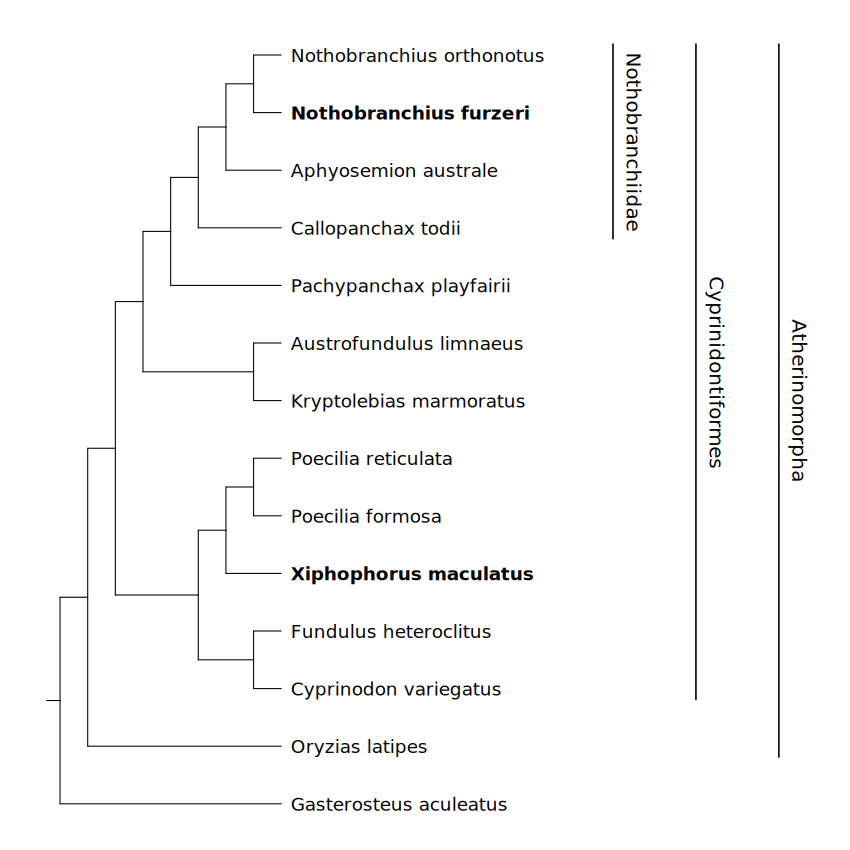
\includegraphics[width=0.9\textwidth]{_Figures/png/species-tree-large-taxa}
	\caption[Cladogram of analysed species]{\textbf{Cladogram of species included in this analysis.} Boldface type indicates species for which new, complete \igh{} locus assemblies were generated for this study; other species were either previously-characterised reference species (\species{G. aculeatus}, \species{O. latipes}) or underwent constant-region characterisation only (all other species). Labelled vertical bars designate higher taxa of interest.}
	\label{fig:species-tree-large-taxa}
\end{figure}

%%%%%%%%%%%%%%%%%%%%%%%%%%%%%%%%%%%%%%%%%%%%%%%%%%%%%%%%%%%%%%%%%%%%%%%%%%%%%%%
% KILLIFISH LOCUS SECTION
%%%%%%%%%%%%%%%%%%%%%%%%%%%%%%%%%%%%%%%%%%%%%%%%%%%%%%%%%%%%%%%%%%%%%%%%%%%%%%%

\section{The \igh{} locus of \nfu}
\label{sec:nfu-locus}

\subsection{Assembling the \Nfu \igh{} locus}
\label{sec:nfu-locus-assembly}

In order to locate and characterise the \nfu \igh{} locus, databases of \vh, \jh, and \ch exon sequences were collated from the published locus sequences of three reference species (zebrafish \parencite{danilova2005zebrafish}, three-spined stickleback \parencite{bao2010stickleback,gambondeza2011stickleback}, and medaka \parencite{magadan2011medaka}) and aligned to the \nfu genome (NFZ2.0) with \program{BLAST} \parencite{altschul1990blast,altschul1997blast}. Genome scaffolds with high-confidence alignments to at least two distinct segment types or covering at least 1\% of the scaffold's total length were retained for downstream analysis as potential locus candidates. In total, one chromosome (chr6) and 6 unincorporated scaffolds were identified as potentially covering part of the locus sequence (\Cref{tab:nfu-locus-scaffolds}), with chromosome 6 bearing the majority of identified gene segments.  %TODO: Add genome accession when available

\begin{table}[bh]
\centering
\caption{\Nfu genome scaffolds containing putative \igh{} locus fragments.}
\begin{threeparttable}
\begin{tabular}{cccccccc}\toprule
\textbf{Scaffold} & \textbf{Total length (kb)} & \textbf{V} & \textbf{J} & \textbf{\cm{}} & \textbf{\cd{}} & \textbf{\cz{}} & Included in locus?\\\midrule
chr6 & 6195.6 & 15 & 7 & 5 & 11 & 0 & Yes\\\midrule
scf10901 & 1.4 & 0 & 0 & 0 & 3 & 0 & Yes\\
scf21863 & 13.5 & 1 & 0 & 0 & 0 & 0 & No\\
scf35954 & 16.3 & 3 & 0 & 0 & 0 & 0 & No\\
scf36277 & 18.9 & 2 & 1 & 0 & 0 & 0 & No\\
scf37083 & 17.7 & 1 & 0 & 0 & 0 & 0 & No\\
scf9157 & 7.2 & 0 & 7 & 4 & 0 & 0 & Yes\\\bottomrule
\end{tabular}

\end{threeparttable}
\label{tab:nfu-locus-scaffolds}
\end{table}

\begin{table}[bh]
\centering
\caption{\Nfu BAC-library inserts containing putative \igh{} locus fragments.}
\begin{threeparttable}
\begin{tabular}{cccccccc}\toprule
\textbf{BAC ID} & \textbf{Insert length (kb)} & \textbf{V} & \textbf{J} & \textbf{\cm{}} & \textbf{\cd{}} & \textbf{\cz{}} & Included in locus?\\\midrule
154G24 & 106.6 & 17 & 1 & 0 & 0  & 0 & No\\
162F04 & 119.4 & 5  & 1 & 0 & 0  & 0 & No\\
165M01 & 110.7 & 15 & 1 & 0 & 0  & 0 & Yes\\
206K13 & 106.7 & 17 & 1 & 0 & 0  & 0 & No\\
208A08 & 103.2 & 17 & 1 & 0 & 0  & 0 & Yes\\
209K12 & 133.0 & 1  & 8 & 4 & 20 & 0 & Yes\\
220O06 & 104.8 & 4  & 1 & 0 & 0  & 0 & No\\
223M21 & 99.3  & 17 & 1 & 0 & 0  & 0 & No\\
248A22 & 47.3  & 7  & 0 & 0 & 0  & 0 & No\\
276N03 & 127.9 & 7  & 0 & 0 & 0  & 0 & Yes\\
277J10 & 120.8 & 17 & 1 & 0 & 0  & 0 & Yes\\
\bottomrule\end{tabular}

\end{threeparttable}
\label{tab:nfu-locus-bacs}
\end{table}

In order to determine which of the putative locus scaffolds were in fact part of the \igh{} locus, integrate these into a contiguous locus sequence, and provide additional information on any missing gene segments, bacterial artificial chromosome insert sequences from the killifish genome project BAC library \parencite{reichwald2015genome} were included in the locus assembly. BAC candidates, whose ends had already been sequenced as part of the genome project, were identified as potentially containing part of the locus sequence on the basis of their ends aligning to promising candidate scaffolds from a previous genome assembly (first round) or to the insert sequences of previously sequenced BAC inserts (second round). Once identified,  BAC candidates were isolated from culture by alkaline lysis, sequenced on an Illumina MiSeq sequencing machine, and assembled and scaffolded with \program{SPAdes} and \program{SSPACE}, respectively. Complete BAC insert assemblies were generated from these scaffolds by manual alignment to overlapping genome scaffolds and other BAC inserts, combined with PCR and Sanger sequencing of intervening sequences.

Finally, the assembled BAC inserts were screened for \igh{} locus segments in the same manner described for genome scaffolds, and passing insert sequences (\Cref{tab:nfu-locus-bacs}) were aligned to and integrated with the identified candidate scaffolds to produce a contiguous locus assembly. To minimise the probability of losing relevant gene segments to assembly errors, priority in the event of a sequence conflict between BACs and scaffolds was given first to any sequence containing a segment missing from the other; if neither the BAC assembly nor the genome scaffolds met this condition, priority was given to the genome scaffold over the BAC assembly. In total, 3 candidate scaffolds (including chromosome 6) and 5 BAC inserts were included in the final locus assembly, while 4 scaffolds and 6 BACs were excluded as likely representing isolated \igh{} orphon segments elsewhere in the genome. The correspondence between the final locus sequence and the sequences used to construct it is shown in \Cref{fig:nfu-locus-aln}.

\begin{figure}
\centering
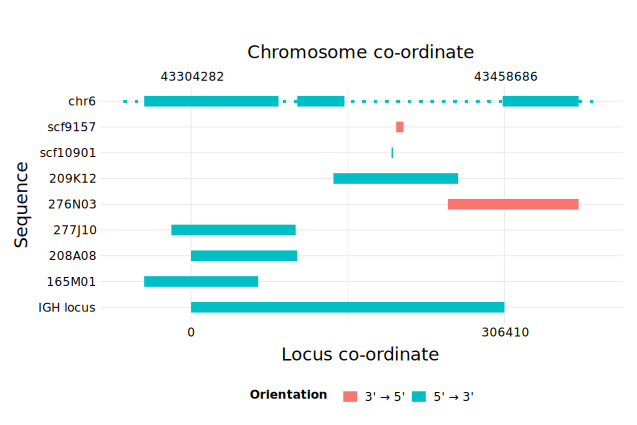
\includegraphics[width=\textwidth]{_Figures/png/nfu-locus-aln}
\caption[Assembling the \Nfu \igh{} locus]{\textbf{Assembling the \Nfu \igh{} locus:} Schematic of genome scaffolds and BAC inserts contributing to the \Nfu \igh{} locus sequence, with their corresponding place within the locus sequence (bottom axis). Internal gaps with dotted lines indicate locus regions with no corresponding locus sequence, as a result of intercalation of BAC or scaffold sequences.}
\label{fig:nfu-locus-aln}
\end{figure}

\subsection{Overall locus structure}
\label{sec:nfu-locus-structure}
	
The turquoise killifish genome contains a single \igh{} locus approximately 306 kilobases in length, located on chromosome 6 of the \Nfu genome (\Cref{fig:nfu-locus-map-a}). This locus comprises two complete subloci, \igh{1} (\kb{155}) and \igh{2} (\kb{118}), present in tandem and each occupying a classic {\vh-\dh-\jh-\ch} translocon configuration. This modified translocon structure, with multiple translocon subloci present in tandem, has been observed in a number of teleost \igh{} loci including catfish, medaka and stickleback \parencite{fillatreau2013astonishing}. Unusually, however, the smaller \igh{2} sublocus in \nfu \igh{} is present in antisense relative to the larger \igh{1}, with the two subloci beginning at opposite ends of the locus and facing each other in the middle (\Cref{fig:nfu-locus-map-b}). Such a multi-orientation locus structure has only previously been observed in medaka, the closest relative of the turquoise killifish to have its locus characterised prior to the present study \parencite{magadan2011medaka}; it is interesting to see this unusual feature reproduced here, raising the question of whether that this ideosyncracy is homologous between the two loci.
	
Compared to other closely-related loci, the killifish locus is relatively sparse and simple, with comparatively low functional complexity relative to its overall size. For example, whereas the stickleback locus fits four subloci, 49 V segments and 10 constant regions into c. \kb{200} \parencite{bao2010stickleback,gambondeza2011stickleback}, the killifish locus, despite being ~50\% longer, contains only 2 subloci, four constant regions and 24 V segments (including pseudogenised Vs). This difference results from the unusually large amount of nonfunctional sequence padding the killifish locus, resulting in large gaps between variable segments and in some cases between constant-region exons (\Cref{fig:nfu-locus-map-b}); this high prevalence of repetitive DNA is consistent with the rest of the TK genome, which comprises more than 60\% repetitive sequence, compared to just over 15\% in stickleback \parencite{yuan2018repeats}. % TODO: Reference for Nfu repeat level - Cui et al ...
	
The two subloci in the turquoise killifish locus are generally highly similar in their functional sequence, with a high degree of synteny between their functional regions (\Cref{fig:nfu-locus-synteny}). The greatest degree of divergence occurs in the \vh and \dh regions, with what appear to be repeated deletion events in IGH2 resulting in a substantially lower number of \vh and \dh segments compared to IGH1; conversely, the \jh and constant regions are almost identical between two subloci. These patterns are discussed in more detail in \Cref{sec:nfu-locus-constant,sec:nfu-locus-variable}.
	
\begin{figure}
	\centering
	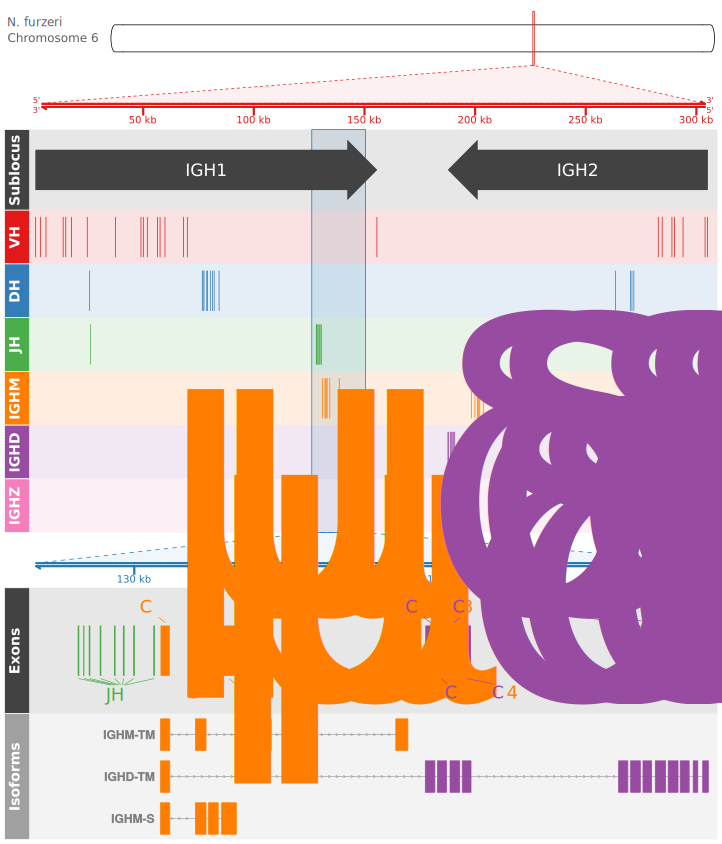
\includegraphics[width=\textwidth]{_Figures/png/nfu-locus-map}
			    \begin{subfigure}{0em}
        \phantomsubcaption{}
        \label{fig:nfu-locus-map-a}
    \end{subfigure}
    \begin{subfigure}{0em}
        \phantomsubcaption{}
        \label{fig:nfu-locus-map-b}
    \end{subfigure}
    \begin{subfigure}{0em}
        \phantomsubcaption{}
        \label{fig:nfu-locus-map-c}
        \end{subfigure}
	\caption[The immunoglobulin heavy chain (\igh{}) locus in \nfu]{\textbf{The immunoglobulin heavy chain (\igh{}) locus in \nfu:} (A) Position of the \igh{} locus on chromosome 6 of the \Nfu genome. (B) Arrangement of \vh, \dh, \jh and constant-region gene segments on the \Nfu \igh{} locus. All segments follow the orientation of their parent sublocus, indicated in the uppermost track. (C) Detailed map of the constant regions of the \textit{IGH1} sublocus, indicating the position and identity of the constant-region exons and the exon composition of expressed \igh{} isoforms in the turquoise killifish.}
	\label{fig:nfu-locus-map}
	\end{figure}
	
\begin{figure}
	\centering
	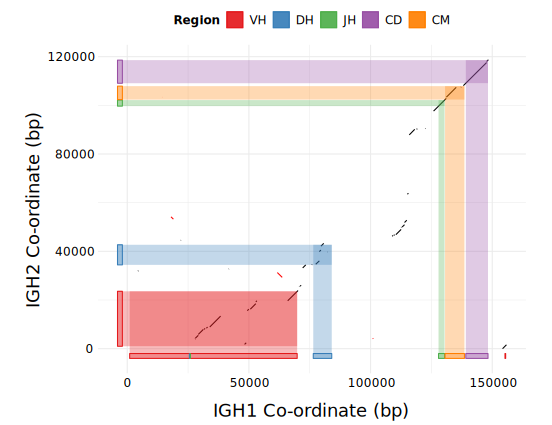
\includegraphics[width=0.9\textwidth]{_Figures/png/nfu-locus-dots}
	\caption[Sequence homology between subloci in \Nfu \igh{}]{\textbf{Sequence homology between subloci in \Nfu \igh{}:} Synteny plot of sequential best matches between \igh{1} and \igh{2} subloci, with gene segment regions indicated by coloured rectangles along each axis.}
	\label{fig:nfu-locus-synteny}
\end{figure}
	
	\subsection{Constant regions}
	\label{sec:nfu-locus-constant}
	
	The \textit{isotype} (also known as the \textit{class}) of an antibody determines its functional role within the immune system, including its possible effector functions and whether it can be secreted \parencite{schroeder2010immunoglobulins}. Three antibody isotypes have been identified to date in teleost fishes: \igh{M}, \igh{D} and \igh{Z} (a.k.a. \igh{T}, \igh{T/Z} or \igh{Z/T}) \parencite{fillatreau2013astonishing,bengten2015fishantibodies,magadan2015fishrepertoires}. Of these, \igh{M} and \igh{D} are highly primitive within the jawed vertebrates and found in most or all other vertebrate groups; within the teleosts, both appear to be universal \parencite{bengten2015fishantibodies}. Conversely, \igh{Z} is a teleost-specific isotype which is absent in other vertebrate taxa; within the teleosts, most characterised \igh{} loci possess \igh{Z}, but at least two (medaka and channel catfish) have been found to lack it \parencite{fillatreau2013astonishing,bengten2015fishantibodies}. In rainbow trout, \igh{Z} has been found to play a specialised mucosal role in the immune system analagous to that of \igh{A} in mammals \parencite{zhang2010igtgut,xu2013igtskin}, and it is widely assumed to play this specialised role throughout the teleosts; it is as yet unclear how mucosal immunity is effected in species lacking \igh{Z}.
	
	In order to investigate constant regions in the \nfu \igh{} locus, putative exon sequences were identified using \program{BLAST} alignments to the reference sequence databases described in \Cref{sec:nfu-locus-assembly}, and intron/exon bounderies were refined through alignment of published RNA-sequencing data from killifish gut (\parencite{smith2017microbiota}, BioProject accession PRJNA379208, young and old untreated groups) using \program{STAR} \Cref{fig:nfu-locus-sashimi}. Strikingly, the \nfu \igh{} locus appears to completely lack any \igh{Z} constant region, with no \cz{} exons or \igh{Z} transmembrane exons being found on either \igh{1} or \igh{2}. Given the widespread prevalence and specialised mucosal role of \igh{Z} in teleosts, its surprising absence in turquoise killifish (\Cref{fig:nfu-locus-map-b}) immediately raises questions about the nature, kinetics and efficacy of mucosal adaptive immunity in this species. The similar absence of \igh{Z} in medaka, which again is the closest relative of \Nfu with a characterised locus, raises further questions about the evolutionary history of \igh{Z} in the Atherinomorpha: does the shared absence of \igh{Z} in these species indicate a single ancestral deletion event, or parallel loss of this important isoform within both the Cyprinodontiformes (including the turquoise killifish) and Beloniformes (including medaka)? This latter question requires higher phylogenetic resolution to address effectively, and is investigated further in \Cref{sec:xma-locus} and \Cref{sec:comparative}.
	
	While \igh{Z} is completely missing from the \Nfu \igh{} locus, \igh{M}, the most primitive and widely-found isotype in jawed vertebrates, is present in its expected location, immediately downstream of the main \jh-region in both subloci. This constant region occupies the standard six-exon configuration, with four \cm{} exons and two transmembrane exons present in series on the chromosome (\Cref{fig:nfu-locus-map-b,fig:nfu-locus-map-c,fig:teleost-igm-exons-a}, \Cref{tab:nfu-ch-coords}). As with other species, both secreted and transmembrane isoforms of \igh{M} are present in the transcriptome, with secreted \igh{M} (\igh{M-S}) consisting of \cm{1-4} (\Cref{fig:nfu-locus-map-c,fig:nfu-locus-sashimi-a,fig:teleost-igm-exons-b}); however, the exon configuration of transmembrane \igh{M} (\igh{M-TM}) deviates from both that seen in mammals (in which exon TM1 is spliced to a cryptic splice site within \cm{4}) and most teleosts (in which the canonical splice site following \cm{3} is used and \cm{4} is excised) \parencite{fillatreau2013astonishing}. Rather, turquoise-killifsh \igh{M-TM} resembles that of medaka, in which both \cm{3} and \cm{4} are excluded and the canonical splice site at the end of \cm{2} is spliced directly to TM1 (\Cref{fig:teleost-igm-exons-c,fig:teleost-igm-exons-d,fig:teleost-igm-exons-e}). This similarity to medaka again raises the possibility that this unusual feature may be a conserved feature of both lineages; however, the underlying mechanism giving rise to this difference in splicing behaviour is unknown.
	
		Unlike \igh{M}, the exon structure of \igh{D} is highly variable across the teleosts, ranging from roughly 7-17 \cd{} exons in addition to the transmembrane domains \parencite{fillatreau2013astonishing}. The core structure of \igh{D} comprises seven \cd{} exons (\cd{1-7}), but some subset of these exons may be missing or duplicated in any given species -- in medaka, for example, \cd{5} is missing in all subloci \parencite{magadan2011medaka}, while in many species (e.g. zebrafish, salmon, and channel catfish) \cd{2-4} are duplicated in two or more tandem blocks \parencite{fillatreau2013astonishing}. This latter configuration is also observed in turquoise killifish, in which the \igh{D} constant region immediately follows \igh{M} in both subloci and has a 

\cd{1}-(\cd{2}-\cd{3}-\cd{4})$_2$-\cd{5}-\cd{6}-\cd{7}-TM1-TM2 

	\noindent configuration, for a total of 12 exons per \igh{D} constant region (\Cref{fig:nfu-locus-map-b,fig:nfu-locus-map-c}, \Cref{tab:nfu-ch-coords}). All of these exons appear to be expressed in tandem, resulting in a much longer transcript than is observed for any isoform of \igh{M} (\Cref{fig:nfu-locus-map-c,fig:nfu-locus-sashimi-b}). As in other teleost species, \igh{D} in the turquoise killifish includes a chimeric \cm{1} exon at the 5' end of the constant-region transcript, for a total of 13 exons per \igh{D-TM} mRNA (\Cref{fig:nfu-locus-sashimi-b}).

	While the best-known form of \igh{D} in teleosts is transmembrane, secreted \igh{D} has been observed in at least two teleost species, with different mechanisms used in each case: in channel catfish, one dedicated sublocus has a dedicated IgD secretory exon in place of the transmembrane exons \parencite{bengten2006catfish}, while in rainbow trout (and possibly some other species like Atlantic salmon and cod) a run-on event at the end of \cd{7} results in the production of a secretory tail in a manner similar to secretory IgZ \parencite{ramirezgomez2012secretoryigd}. However, neither a specialised secretory exon nor a \cd{7} secretory tail could be detected in turquoise killifish, suggesting that IgD may only be expressed in transmembrane form in this species.
	
	In the case of both \igh{M} and \igh{D}, the constant regions are present in their expected configuration in each sublocus and are highly similar in sequence between the subloci, with an average of 98.4\% nucleotide sequence identity for corresponding IgM exons and 99.3\% for corresponding IgD exons (\Cref{fig:nfu-ch-aln} and \Cref{tab:nfu-ch-aln}) in pairwise Needleman-Wunsch alignments \parencite{needleman1970align}. This high level of similarity indicates either a very recent duplication event to produce the second sublocus or a high level of sequence conservation in both subloci, with the latter explanation suggesting that both subloci continue to be functional and active in the immune system.
	
	\begin{figure}
	\centering
		    \begin{subfigure}{0em}
        \phantomsubcaption{}
        \label{fig:teleost-igm-exons-a}
    \end{subfigure}
    \begin{subfigure}{0em}
        \phantomsubcaption{}
        \label{fig:teleost-igm-exons-b}
    \end{subfigure}
    \begin{subfigure}{0em}
        \phantomsubcaption{}
        \label{fig:teleost-igm-exons-c}
    \end{subfigure}
    \begin{subfigure}{0em}
        \phantomsubcaption{}
        \label{fig:teleost-igm-exons-d}
    \end{subfigure}
    \begin{subfigure}{0em}
        \phantomsubcaption{}
        \label{fig:teleost-igm-exons-e}
    \end{subfigure}
	\includegraphics[width=0.8\textwidth]{_Figures/png_edited/teleost-igm-exons}
	\caption[IgM exon usage in other vertebrates]{\textbf{\igh{M} exon usage in other vertebrates:} Schematic of \igh{M} splice patterns in different isoforms and taxonomic groups; (A) standard genomic (pre-splicing) configuration of \igh{M}, following VDJ recombination; (B) exon configuration of secreted \igh{M} (\igh{M-S}) in tetrapods and teleosts; (C) exon configuration of transmembrane \igh{M} (\igh{M-TM}) in tetrapods, demonstrating the use of a cryptic splice site in \cm{4}; (D) standard \igh{M-TM} exon configuration in teleosts, demonstrating the direct splicing of \cm{3} to TM1 and exclusion of \cm{4}; (E) unusual \igh{M-TM} exon configuration observed in medaka, in which both \cm{3} and \cm{4} are excluded. Figure adapted from Fillatreau \textit{et al.} (2013).}
	\label{fig:teleost-igm-exons}
	\end{figure}
	
	\begin{figure}
	\centering
		\begin{subfigure}{0em}
        \phantomsubcaption{}
        \label{fig:nfu-locus-sashimi-a}
    \end{subfigure}
    \begin{subfigure}{0em}
        \phantomsubcaption{}
        \label{fig:nfu-locus-sashimi-b}
    \end{subfigure}
	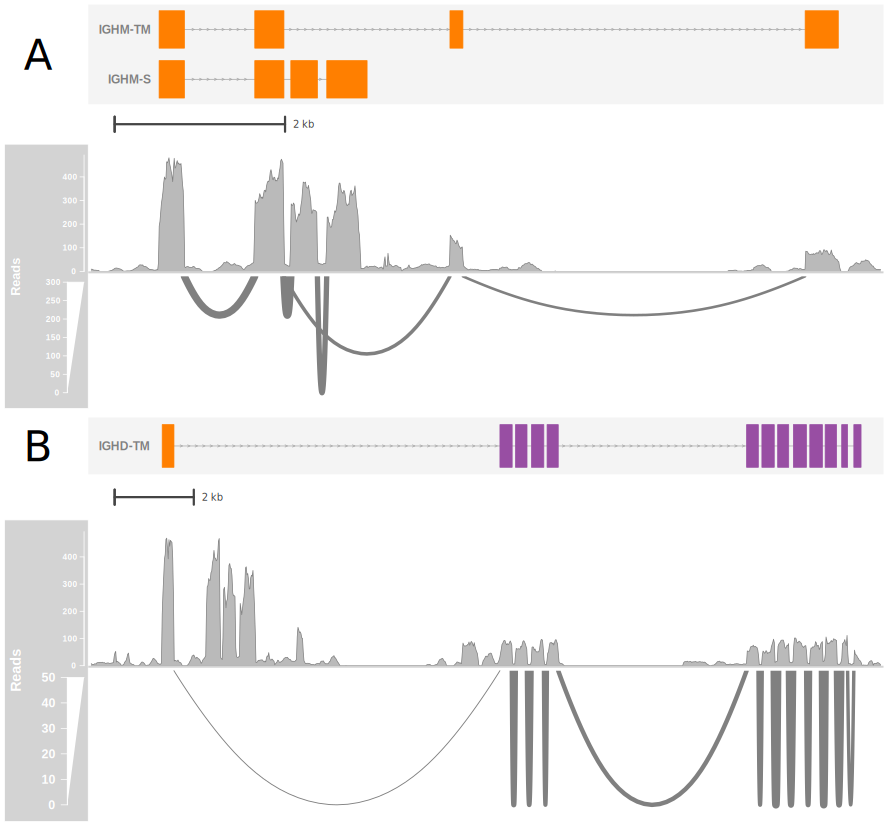
\includegraphics[width=\textwidth]{_Figures/png/nfu-locus-sashimi}
	\caption[Constant-region isoforms in \Nfu]{\textbf{Constant-region isoforms in \Nfu:} Coverage and sashimi plots of \program{STAR}-aligned RNA-seq reads from \Nfu gut samples \parencite{smith2017microbiota}, demonstrating the splicing behaviour of \igh{1} constant-region isoforms. (A) \igh{M} exon splicing, showing alternative splicing patterns of \igh{M-TM} and \igh{M-S}; (B) \igh{D} exon splicing, including chimeric splicing of \cm{1} to \cd{1}.}
	\label{fig:nfu-locus-sashimi}
	\end{figure}
	
	\begin{figure}
	\centering
	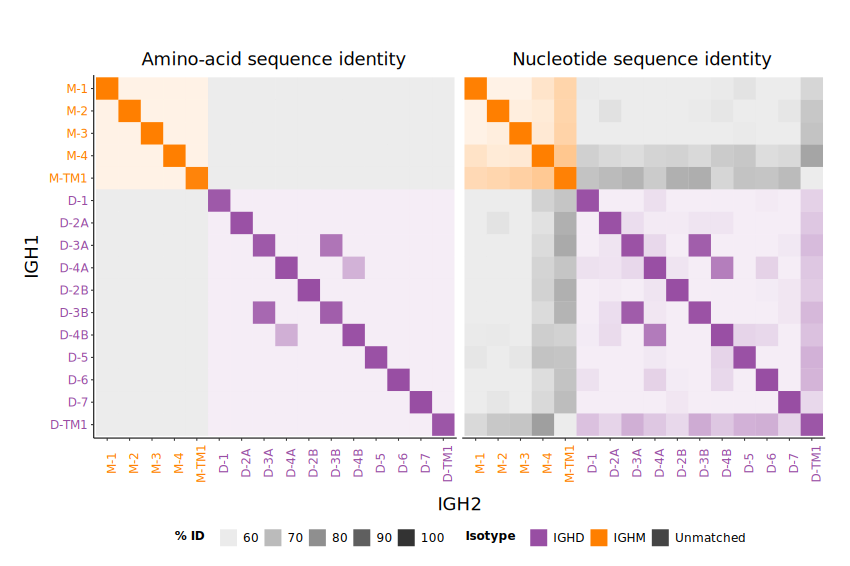
\includegraphics[width = \textwidth]{_Figures/png/nfu-ch-aln}
	\caption[Cross-sublocus sequence similarity in constant-region exons in \Nfu \textit{IGH}]{\textbf{Cross-sublocus sequence similarity in constant-region exons in \Nfu:} Heatmap of percentage sequence identity between amino-acid (right) and nucleotide (left) sequences of constant-region exons (excluding \igh{M-TM2} and \igh{D-TM2}) from the two subloci of \Nfu \textit{IGH}, calculated using pairwise Needleman-Wunsch global alignments..}
	\label{fig:nfu-ch-aln}
	\end{figure}
	
	\begin{table}\centering
		\caption[Cross-sublocus sequence similarity between corresponding constant-region exons in \Nfu \textit{IGH}]{\textbf{Cross-sublocus sequence similarity in constant-region exons in \Nfu:} Percentage sequence identities of pairwise Needleman-Wunsch global alignments between nucleotide (NT) or amino-acid (AA) sequences of corresponding exons from the two subloci of \Nfu \textit{IGH}.}
	% latex table generated in R 3.5.1 by xtable 1.8-3 package
% Wed Nov 21 11:59:38 2018
\begin{tabular}{llrr}
  \toprule Isotype & Exon & NT & AA \\ 
  \midrule M & 1 & 99.66 & 100.00 \\ 
  M & 2 & 100.00 & 100.00 \\ 
  M & 3 & 100.00 & 100.00 \\ 
  M & 4 & 100.00 & 100.00 \\ 
  M & TM1 & 99.34 & 98.00 \\ 
  M & TM2 & 91.67 & 100.00 \\ 
  D & 1 & 99.03 & 97.06 \\ 
  D & 2A & 98.97 & 98.96 \\ 
  D & 3A & 98.72 & 97.09 \\ 
  D & 4A & 99.65 & 98.92 \\ 
  D & 2B & 100.00 & 100.00 \\ 
  D & 3B & 98.72 & 96.12 \\ 
  D & 4B & 99.64 & 98.91 \\ 
  D & 5 & 99.09 & 99.08 \\ 
  D & 6 & 100.00 & 100.00 \\ 
  D & 7 & 100.00 & 100.00 \\ 
  D & TM1 & 97.99 & 97.96 \\ 
  D & TM2 & 99.44 & 100.00 \\ 
   \bottomrule \end{tabular}

	\label{tab:nfu-ch-aln}
	\end{table}
	
\begin{table}\centering
    \caption{Co-ordinate table of constant-region exons in the \nfu \igh{} locus.}
    	% latex table generated in R 3.5.2 by xtable 1.8-3 package
% Tue Jan 15 17:07:52 2019
\begin{tabular}{llrrrl}
  \toprule Name & Isotype & Start & End & Length & Strand \\ 
  \midrule IGH1M-1 & M & 130848 & 131144 & 297 & + \\ 
  IGH1M-2 & M & 131971 & 132312 & 342 & + \\ 
  IGH1M-3 & M & 132394 & 132705 & 312 & + \\ 
  IGH1M-4 & M & 132816 & 133288 & 473 & + \\ 
  IGH1M-TM1 & M & 134262 & 134413 & 152 & + \\ 
  IGH1M-TM2 & M & 138431 & 138819 & 389 & + \\ 
  IGH1D-1 & D & 139381 & 139689 & 309 & + \\ 
  IGH1D-2A & D & 139774 & 140064 & 291 & + \\ 
  IGH1D-3A & D & 140178 & 140489 & 312 & + \\ 
  IGH1D-4A & D & 140572 & 140853 & 282 & + \\ 
  IGH1D-2B & D & 145613 & 145909 & 297 & + \\ 
  IGH1D-3B & D & 146000 & 146311 & 312 & + \\ 
  IGH1D-4B & D & 146398 & 146676 & 279 & + \\ 
  IGH1D-5 & D & 146795 & 147124 & 330 & + \\ 
  IGH1D-6 & D & 147210 & 147527 & 318 & + \\ 
  IGH1D-7 & D & 147598 & 147885 & 288 & + \\ 
  IGH1D-TM1 & D & 148016 & 148164 & 149 & + \\ 
  IGH1D-TM2 & D & 148323 & 148504 & 182 & + \\ 
  IGH2D-TM2 & D & 187624 & 187803 & 180 & - \\ 
  IGH2D-TM1 & D & 187963 & 188111 & 149 & - \\ 
  IGH2D-7 & D & 188658 & 188945 & 288 & - \\ 
  IGH2D-6 & D & 189016 & 189333 & 318 & - \\ 
  IGH2D-5 & D & 189419 & 189748 & 330 & - \\ 
  IGH2D-4B & D & 189867 & 190145 & 279 & - \\ 
  IGH2D-3B & D & 190232 & 190543 & 312 & - \\ 
  IGH2D-2B & D & 190636 & 190932 & 297 & - \\ 
  IGH2D-4A & D & 195644 & 195925 & 282 & - \\ 
  IGH2D-3A & D & 196008 & 196319 & 312 & - \\ 
  IGH2D-2A & D & 196433 & 196723 & 291 & - \\ 
  IGH2D-1 & D & 196808 & 197116 & 309 & - \\ 
  IGH2M-TM2 & M & 198315 & 198506 & 192 & - \\ 
  IGH2M-TM1 & M & 199834 & 199985 & 152 & - \\ 
  IGH2M-4 & M & 200953 & 201425 & 473 & - \\ 
  IGH2M-3 & M & 201536 & 201847 & 312 & - \\ 
  IGH2M-2 & M & 201929 & 202270 & 342 & - \\ 
  IGH2M-1 & M & 203549 & 203845 & 297 & - \\ 
   \bottomrule \end{tabular}

    \label{tab:nfu-ch-coords}
\end{table}

\subsection{Variable regions}
\label{sec:nfu-locus-variable}
	
Variable-region gene segments in the killifish \igh{} locus were identified with a variety of methods, depending on the type of gene segment being analysed. \vh candidates were identified probabilistically using Hidden Markov Models constructed by \program{nhmmer} \parencite{wheeler2013nhmmer} from \program{PRANK} \parencite{loytynoja2014prank} multiple-sequence alignments of reference sequences, with the 3'-ends of each V-exon identified by the presence of a recombination-signal sequence (RSS) \parencite{schroeder2010immunoglobulins} and the 5'-ends refined using \program{IMGT-DomainGapAlign} \parencite{ehrenmann2011domaingapalign}. \jh candidates were also identified using \program{nhmmer}, with segment ends identified by the presence of an RSS (5') and a \sequence{GTA} splice-site motif (3') \parencite{magadan2011medaka}. Finally, \dh-segments, being too short and variable in sequence for HMM-based approaches to be effective, were identified by searching for pairs of flanking RSS sequences in opposite orientation, using fuzzy pattern-matching (with EMBOSS \program{FUZZNUC} \parencite{rice2000emboss}) to conserved RSS sequence motifs.
	 
In total, 24 \vh-segments, 14 \dh-segments and 17 \jh-segments were identified in the \Nfu locus (\Cref{tab:nfu-vh-coords,tab:nfu-dh-coords-seg,tab:nfu-jh-coords-seg}), of which the majority (17 \vh, 10 \dh and 8 \jh) were present in \igh{1}. Of the \vh segments identified, three contain premature STOP codons, though none is out-of-frame; conversely, all the \dh and \jh segments identified appear to be in-frame and functional, with no premature STOP codons. However, in all cases a minority of segments contain RSS sequences that deviate significantly from the expected consensus sequence (\Cref{tab:nfu-vh-coords,tab:nfu-dh-coords-rss5,tab:nfu-dh-coords-rss3,tab:nfu-jh-coords-rss}); it is unclear whether these sequences can recombine to successfully produce mature VDJ sequences \textit{in vivo}. In the case of the \vh segments, of the six sequences without clearly functional RSS sequences, three also contain premature STOP codons, suggesting the changes to the RSS in these cases may arise from relaxed purifying selection on already-pseudogenised sequences.

Apart from these few exceptions, however, the recombination signal sequences (RSS) marking the ends of the \vh, \dh and \jh gene segments in the \Nfu locus otherwise strongly resemble those of other characterised teleosts, which in turn resemble those of non-teleost loci (\Cref{fig:nfu-rss-seqlogo-all,fig:nfu-rss-seqlogo-sep}). The overall heptamer and nonamer consensus sequences (\texttt{CACAGTG} for heptamers and \texttt{ACAAAAACC} for nonamers) closely matched those expected from the literature \parencite{schroeder2010immunoglobulins}, while in 88\% of cases the spacer region was within 1bp of the expected length (12bp for D-RSSs, 23bp for V- and J-RSSs); unexpectedly, the greatest number of \vh-RSSs had a 22bp (rather than 23bp) spacer, but this is unlikely to interfere with RSS functionality. Overall, the RSSs in the turquoise killifish appear to be supporting the normal operation of VDJ-recombination in this species.

Of the \vh, \dh and \jh segments identified, all but one of each type of segment is located within contiguous V-, D-, and J-regions within each sublocus, supporting a modified translocon configuration for killifish \igh. The exceptions to this are \igh{1D01} and \igh{1J01}, which are embedded within the \igh{1} V-region, and a single \vh segment located in between the \igh{D} contant regions of the two subloci (\Cref{fig:nfu-locus-map-b}). The unusual location of \igh{1D01} and \igh{1J01} may represent the result of a transposition event within the \igh{} locus; however, their close colocalisation and 5' position within the \igh{1} sublocus, as well as the fact that neither has a close paralogue in \igh{2} (\Cref{fig:nfu-dj-alignment-b}), suggest that they may instead represent the remnant of a formerly present \igh{Z} constant region, as these typically have dedicated D/J segments independent of those serving \igh{M}. Given its forward orientation, meanwhile, the orphaned \vh-segment was assigned to the \igh{1} sublocus as \igh{1V1-07}; however, if annotated correctly, it is unlikely to successfully recombine with segments in either sublocus due to its unusual location.
		
\begin{table}[hb]
	\centering
	\begin{threeparttable}
	\centering
	\caption{Number of functional \vh-segments and \vh-families in other teleost species.}
	\label{tab:teleost-vh-counts}
	\begin{tabular}{ccccc}\toprule
	\multirow{2}{*}{	\textbf{Common Name}} & \multirow{2}{*}{\textbf{Species}} & \textbf{\# Functional} & \textbf{	\# \vh} & \multirow{2}{*}{\textbf{Source}} \\
	& & \textbf{\vh Segments} & \textbf{Families} & \\\midrule
	Zebrafish & \textit{Danio rerio} & 39 & 13\,\tnote{1} & \parencite{magadan2015fishrepertoires} \\
	Grasscarp & \textit{Ctenopharyngodon idella} & 8 & 5\,\tnote{2} & \parencite{xiao2010grasscarp} \\
	Fugu & \textit{Takifugu rubripes} & 34 & 3 & \parencite{magadan2015fishrepertoires} \\
	Medaka & \textit{Oryzias latipes} & 35 & 6 & \parencite{fillatreau2013astonishing,magadan2011medaka} \\
	Stickleback & \textit{Gasterosteus aculeatus} & 49 & 4 & \parencite{magadan2015fishrepertoires} \\
	Turquoise killifish & \textit{Nothobranchius furzeri} & 21\,\tnote{3} & 6 & -- \\
	\bottomrule\end{tabular}
	\begin{tablenotes}
	\item[1] \vh families in zebrafish identified based on 70\% (rather than 80\%) sequence identity.
	\item[2] It is not clear what clustering method or threshold was used to identify \vh families in grasscarp.
	\item[3] Excluding \vh segments with nonsense or frameshift mutations, but not those with uncertain or missing RSS sequences.
	\end{tablenotes}
	\end{threeparttable}
\end{table}
	
\vh sequences within an \igh{} locus are conventionally grouped into families on the basis of nucleotide sequence identity, with a typical identity cutoff of 80\% \parencite{magadan2015fishrepertoires}. In order to group the \Nfu \vh genes into families, pairwise Needleman-Wunsch global alignments were performed on each pair of \vh sequences to obtain pairwise identity scores, followed by single-linkage clustering on the resulting identity matrix. Cutting the dendrogram at 80\% sequence identity revealed a total of six \vh families, of which four contained more than one \vh segment (\Cref{fig:nfu-vh-families}); this number of \vh families in the \Nfu locus is roughly in line with those found in related species (\Cref{tab:teleost-vh-counts}). Of these, V1 and V2 make up the bulk (42\% and 29\% respectively) of the \vh segments in the locus. V2 and V4 are highly similar, and all the members of V4 are pseudogenised by premature STOP codons; it may therefore be more appropriate to regard V4 as a pseudogenised subfamily of V2 than as a \vh family in its own right.

The total number of functional \vh segments in the killifish locus is unusually small in comparison to the total numbers observed in many other teleost species (\Cref{tab:teleost-vh-counts}); however, the number of segments per sublocus is in line with the numbers seen in closely-related species (2 to 12 in medaka, 6 to 18 in stickleback), with the overall difference mainly arising from a difference in the number of subloci per locus. A similar pattern is observed with \dh and \jh segments, with similar numbers of segments per sublocus in killifish and closely-related species, especially medaka. It therefore appears that the per-sublocus segment diversity available to the turquoise killifish is similar to that of previously characterised species, with any difference in total available diversity at this level arising from differences in the number of functional subloci rather than the size of the V/D/J-regions \textit{per se}.

As can be seen from \Cref{fig:nfu-locus-synteny}, much of the V-, D- and especially J-region sequence in the \Nfu locus is syntenic between the two \igh{} subloci, with downstream portions of the \igh{2} V-region corresponding to downstream parts of the \igh{1} region. Of the seven \vh segments in \igh{2}, six have a correspending segment on \igh{1} with which they share at least 97\% sequence identity (\Cref{fig:nfu-vh-families}), and these partner segments are largely (though not entirely) colinear in their ordering between the two subloci. A similar pattern can be observed for the D- and (especially) the J-regions: of the four \dh segments detectable in \igh{2}, three (\igh{2D02} to \igh{2D04}) are identical with another block of adjacent \dh segments in \igh{1} (\igh{1D05} to \igh{1D07}), while the \jh-regions exhibit almost complete sequence identity between the eight \jh segments of the main \jh region in \igh{1} and the eight \jh segments in \igh{2} (\Cref{fig:nfu-dj-alignment}).
		
Nevertheless, as is clear from \Cref{fig:nfu-locus-synteny}, there are large portions the \igh{1} variable region, including the first 25 kilobases of the V-region, for which no corresponding sequence exists in \textit{IGH2}, and there are many \vh and \dh segments in \igh{1} (and a much smaller number in \igh{2}) for which no close homologue exists in the other sublocus. Taken together, these data are consistent with a model in which \igh{2} was produced via duplication and inversion of all or part of \igh{1}, followed by subsequent deletion events in the redundant, and structurally volatile, \igh{2} \vh and \dh regions. However, it is not clear at present how to distinguish between this model and an alternative one of expansion in \igh{1}, or to identify why the \jh region is so much more conserved between subloci than either the \vh or \jh regions.

	
	\begin{figure}
	\centering
	\begin{subfigure}{0em}
	\phantomsubcaption{}
    \label{fig:nfu-vh-families-a}
    \end{subfigure}
    \begin{subfigure}{0em}
    \phantomsubcaption{}
    \label{fig:nfu-vh-families-b}
    \end{subfigure}
	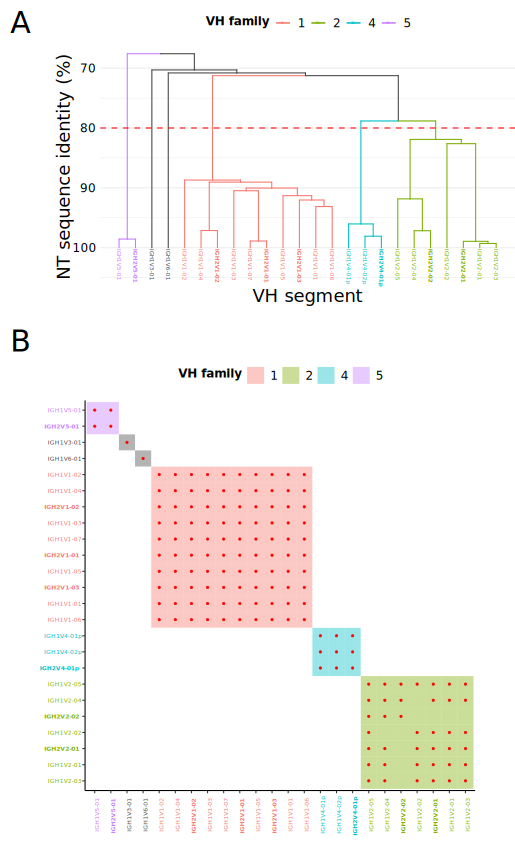
\includegraphics[width=0.8\textwidth]{_Figures/png/nfu-vh-families.png}
	\caption[\vh families in the in \Nfu \igh{} locus]{\textbf{\vh families in the in \Nfu \igh{} locus:} (A) Dendrogram of sequence similarity of \vh segments in the \Nfu \igh{} locus, arranged by single-linkage clustering on nucleotide sequence identity. The red line indicates the 80\% cutoff point for family assignment, while branch colour indicates family membership. (B) Heatmap of family relationships among \Nfu \vh segments, with coloured shading indicating families and red dots indicating pairwise nucleotide sequence identity of at least 80\%. In both subfigures, \vh families containing multiple segments are coloured, single-segment families are in grey, and segments from the \igh{2} sublocus are displayed in \textbf{boldface}.}
	\label{fig:nfu-vh-families}
	\end{figure}

\begin{figure}
\centering
	\centering
	\begin{subfigure}{0em}
	\phantomsubcaption{}
    \label{fig:nfu-dj-alignment-a}
    \end{subfigure}
    \begin{subfigure}{0em}
    \phantomsubcaption{}
    \label{fig:nfu-dj-alignment-b}
    \end{subfigure}

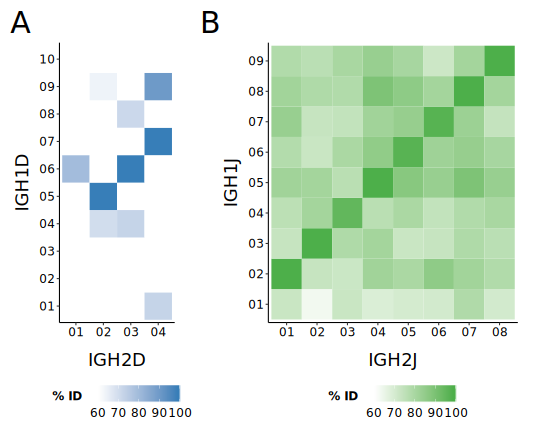
\includegraphics[width=0.6\textwidth]{_Figures/png/nfu-dj-aln}
\caption[Cross-sublocus sequence similarity in \dh and \jh gene segments in \Nfu]{\textbf{Cross-sublocus sequence similarity in \dh and \jh gene segments in \Nfu:} Heatmap of percentage nucleotide sequence identities of Needleman-Wunsch global alignments between (A) \dh and (B) \jh gene segments in IGH1 vs IGH2, revealing syntenic runs of highly similar sequences across both subloci.}
\label{fig:nfu-dj-alignment}
\end{figure}	
	
	\begin{figure}
	\centering
	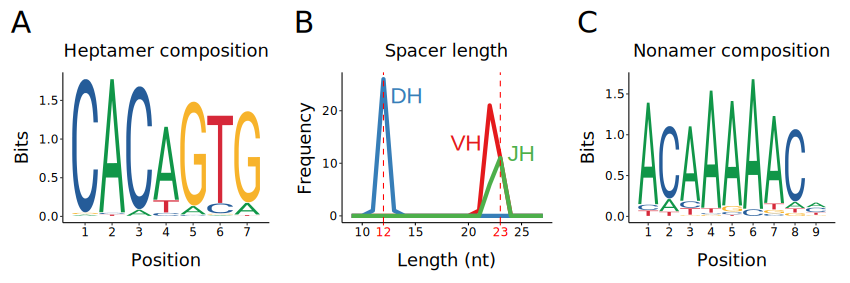
\includegraphics[width=\textwidth]{_Figures/png/nfu-rss-seqlogo-all}
	\caption[Recombination signal sequences in the \Nfu \textit{IGH} locus]{\textbf{Recombination signal sequences in the \Nfu \textit{IGH} locus:} (A) Sequence composition of conserved heptamer sequences across all \Nfu heavy-chain RSSs; (B) length distribution of unconserved spacer sequences in \Nfu heavy-chain RSSs; (C) sequence composition of conserved heptamer sequences across all \Nfu heavy-chain RSSs.}
	\label{fig:nfu-rss-seqlogo-all}
	\end{figure}
	
\begin{figure}
	\centering
	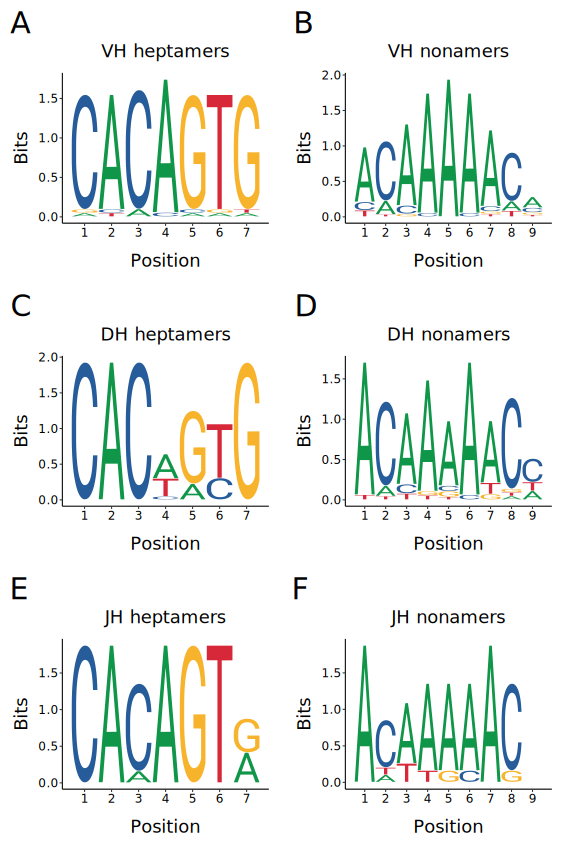
\includegraphics[width=0.9\textwidth]{_Figures/png/nfu-rss-seqlogo-sep}
	\caption[\Nfu recombination signal sequences by segment type]{\textbf{\Nfu recombination signal sequences by segment type:} Sequence composition of conserved heptamer (A,C,E) and nonamer (B,D,F) sequences from \Nfu heavy-chain RSSs associated with \vh (A,B), \dh (C,D) or \jh (E,F) gene segments.}
	\label{fig:nfu-rss-seqlogo-sep}
	\end{figure}

\FloatBarrier

\afterpage{%
    \begin{landscape}
        \centering
        \vspace*{\fill}
        \scriptsize
		% latex table generated in R 3.5.2 by xtable 1.8-3 package
% Fri Jan  4 11:18:28 2019
\begin{tabular}{lrrrlrlrlrrl}
  \toprule Name & Start & End & Length & Strand & RSS Start & Heptamer & Spacer Length & Nonamer & RSS End & RSS Length & Comment \\ 
  \midrule IGH1V1-01 & 1252 & 1540 & 289 & + & 1541 & CACAGTG & 22 & ACAAAAACC & 1578 & 38 &  \\ 
  IGH1V1-02 & 3365 & 3656 & 292 & + & 3657 & CACAGTG & 22 & ACAAAAACC & 3694 & 38 &  \\ 
  IGH1V2-01 & 5907 & 6201 & 295 & + & 6202 & CACAGAA & 15 & ACAAAAACT & 6232 & 31 &  \\ 
  IGH1V1-03 & 13690 & 13964 & 275 & + & 13965 & CACAGTG & 22 & ACAAAAACC & 14002 & 38 &  \\ 
  IGH1V3-01 & 14862 & 15162 & 301 & + & 15163 & CACAGTG & 23 & ACAAAAACC & 15201 & 39 &  \\ 
  IGH1V2-02 & 17433 & 17730 & 298 & + & 17731 & CACAATG & 23 & ACAAAAACC & 17769 & 39 &  \\ 
  IGH1V4-01 & 24566 & 24837 & 272 & + & 24838 & CGCAGTG & 22 & CCACAAACC & 24875 & 38 & Nonsense mutation \\ 
  IGH1V1-04 & 37305 & 37596 & 292 & + & 37597 & CACAGTG & 22 & ACAAAAACC & 37634 & 38 &  \\ 
  IGH1V2-03 & 48845 & 49139 & 295 & + & 49140 & CACAGTG & 23 & TCAAAAACT & 49178 & 39 &  \\ 
  IGH1V1-05 & 49909 & 50197 & 289 & + & 50198 & CACAGTG & 22 & ACAAAAACC & 50235 & 38 &  \\ 
  IGH1V5-01 & 51710 & 51998 & 289 & + & 51999 & CACAGTG & 22 & ACAAAAACT & 52036 & 38 &  \\ 
  IGH1V2-04 & 56322 & 56616 & 295 & + & 56617 & CACAGTG & 23 & ACAAAAACC & 56655 & 39 &  \\ 
  IGH1V6-01 & 57465 & 57762 & 298 & + & 57763 & CACAGTG & 21 & ACTAAATCT & 57799 & 37 &  \\ 
  IGH1V1-06 & 59678 & 59966 & 289 & + & 59967 & CACAGTG & 22 & ACAAAAACC & 60004 & 38 &  \\ 
  IGH1V4-02 & 68017 & 68288 & 272 & + & 68289 & TGCAGTG & 22 & TCACAAACC & 68326 & 38 & Nonsense mutation \\ 
  IGH1V2-05 & 69787 & 70084 & 298 & + & 70085 & CACAGTG & 23 & ACAAAAACC & 70123 & 39 &  \\ 
  IGH1V1-07 & 155485 & 155763 & 279 & + & 155764 & CACAGTG & 22 & TCAAAACCC & 155801 & 38 &  \\ 
  IGH2V2-02 & 282620 & 282914 & 295 & - & 282915 & CACAGTG & 23 & ACAAAAACC & 282953 & 39 &  \\ 
  IGH2V4-01 & 284404 & 284675 & 272 & - & 284676 & TGCAGTG & 22 & TCACAAACC & 284713 & 38 & Nonsense mutation \\ 
  IGH2V5-01 & 288808 & 289096 & 289 & - & 289097 & CACAGTG & 22 & ACAGAAACT & 289134 & 38 &  \\ 
  IGH2V1-03 & 289977 & 290271 & 295 & - & 290272 & CACAGTG & 22 & ACAAAAACC & 290309 & 38 &  \\ 
  IGH2V1-02 & 293835 & 294126 & 292 & - & 294127 & CACAGTG & 22 & ACAAAAACC & 294164 & 38 &  \\ 
  IGH2V2-01 & 303780 & 304074 & 295 & - & 304075 & CAGGGCC & 24 & AGCACAAAG & 304114 & 40 &  \\ 
  IGH2V1-01 & 304926 & 305204 & 279 & - & 305205 & CACAGTG & 22 & TCAAAACCC & 305242 & 38 &  \\ 
   \bottomrule \end{tabular}

		\normalsize\vspace{1em}
        \captionof{table}{Co-ordinate table of \vh segments in the \nfu \igh{} locus.}
        \label{tab:nfu-vh-coords}
        \vspace*{\fill}
    \end{landscape}
}

\afterpage{%
        \centering
        \captionof{table}{Co-ordinate table of \dh segments in the \nfu \igh{} locus.}\vspace{-0.3em}
        \label{tab:nfu-dh-coords-seg}
        \scriptsize
		% latex table generated in R 3.5.2 by xtable 1.8-3 package
% Tue Jan 15 17:07:52 2019
\begin{tabular}{lrlrrl}
  \toprule Name & Start & NT Sequence & End & Length & Strand \\ 
  \midrule IGH1D01 & 25782 & ATACGTACTTTCGTGGTATATAGAGA & 25807 & 26 & + \\ 
  IGH1D02 & 76700 & GATATCTGGGTGGGGG & 76715 & 16 & + \\ 
  IGH1D03 & 77027 & TGAAATGATTAC & 77038 & 12 & + \\ 
  IGH1D04 & 77476 & TCGCGTAGCGGC & 77487 & 12 & + \\ 
  IGH1D05 & 78717 & GAAACCACGGCAGC & 78730 & 14 & + \\ 
  IGH1D06 & 79049 & TTTATAGCGGCTAC & 79062 & 14 & + \\ 
  IGH1D07 & 80417 & CAGACTGGAGA & 80427 & 11 & + \\ 
  IGH1D08 & 81362 & TTCATGGCAGCCAC & 81375 & 14 & + \\ 
  IGH1D09 & 82067 & CAGACTGGAGC & 82077 & 11 & + \\ 
  IGH1D10 & 84282 & TGGGGTGGCAGC & 84293 & 12 & + \\ 
  IGH2D04 & 263497 & CAGACTGGAGA & 263507 & 11 & - \\ 
  IGH2D03 & 270243 & TTTATAGCGGCTAC & 270256 & 14 & - \\ 
  IGH2D02 & 270878 & GAAACCACGGCAGC & 270891 & 14 & - \\ 
  IGH2D01 & 271749 & GACTTTTACTAC & 271760 & 12 & - \\ 
   \bottomrule \end{tabular}

		\normalsize\vspace{1em}
        \captionof{table}{Co-ordinate table of \dh 5'-RSSs in the \nfu \igh{} locus.}\vspace{-0.3em}
        \label{tab:nfu-dh-coords-rss5}
        \scriptsize
        	% latex table generated in R 3.5.2 by xtable 1.8-3 package
% Fri Jan  4 11:18:28 2019
\begin{tabular}{lrlrlrr}
  \toprule Name & 5'-RSS Start & Nonamer & Spacer Length & Heptamer & 5'-RSS End & Length \\ 
  \midrule IGH1D01 & 25754 & GGTTGTTGT & 12 & CACTGTG & 25781 & 28 \\ 
  IGH1D02 & 76672 & AGTTTTTGA & 12 & CACAGTG & 76699 & 28 \\ 
  IGH1D03 & 76999 & TGTTGTTGT & 12 & CACAGTG & 77026 & 28 \\ 
  IGH1D04 & 77448 & AGTTTTTGT & 12 & CACGGTG & 77475 & 28 \\ 
  IGH1D05 & 78688 & GATGTTTTT & 13 & CACAGTG & 78716 & 29 \\ 
  IGH1D06 & 79021 & TGTTTTTGT & 12 & CGCTGTG & 79048 & 28 \\ 
  IGH1D07 & 80417 & AGTTTTGGT & 12 & CACAGTG & 80444 & 28 \\ 
  IGH1D08 & 81334 & TGTTTTTGT & 12 & CGCTGTG & 81361 & 28 \\ 
  IGH1D09 & 82039 & AGTTTTGGT & 12 & CACAGTG & 82066 & 28 \\ 
  IGH1D10 & 84254 & TCATTCATT & 12 & CACTGTG & 84281 & 28 \\ 
  IGH2D04 & 263497 & AGTTTTGGT & 12 & CACAGTG & 263524 & 28 \\ 
  IGH2D03 & 270215 & TGTTTTTGT & 12 & CGCTGTG & 270242 & 28 \\ 
  IGH2D02 & 270850 & TGTTTTTGT & 12 & CACAGTG & 270877 & 28 \\ 
  IGH2D01 & 271721 & AGTTTTTAT & 12 & CATGGTG & 271748 & 28 \\ 
   \bottomrule \end{tabular}

        	\normalsize\vspace{1em}
        \captionof{table}{Co-ordinate table of \dh 3'-RSSs in the \nfu \igh{} locus.}\vspace{-0.3em}
        \label{tab:nfu-dh-coords-rss3}
        \scriptsize
		% latex table generated in R 3.5.2 by xtable 1.8-3 package
% Tue Jan 15 17:07:52 2019
\begin{tabular}{lrlrlrr}
  \toprule Name & 3'-RSS Start & Heptamer & Spacer Length & Nonamer & 3'-RSS End & Length \\ 
  \midrule IGH1D01 & 25808 & CACAGTG & 12 & ACAAAAACC & 25835 & 28 \\ 
  IGH1D02 & 76716 & CACAGTG & 12 & ACAAAAACC & 76743 & 28 \\ 
  IGH1D03 & 77039 & CACTGTG & 11 & AATATAACC & 77065 & 27 \\ 
  IGH1D04 & 77488 & CACAGCG & 12 & ACATAAAAC & 77515 & 28 \\ 
  IGH1D05 & 78731 & CACAGCG & 12 & ACAAAAGCC & 78758 & 28 \\ 
  IGH1D06 & 79063 & CACTGTG & 12 & ACAAGATCC & 79090 & 28 \\ 
  IGH1D07 & 80428 & CACAACG & 12 & ACAAAAACC & 80455 & 28 \\ 
  IGH1D08 & 81376 & CACTGTG & 12 & ACAAAATCC & 81403 & 28 \\ 
  IGH1D09 & 82078 & CACAATG & 12 & ACAAAAACC & 82105 & 28 \\ 
  IGH1D10 & 84294 & CACAGTG & 12 & ACAAAAACC & 84321 & 28 \\ 
  IGH2D04 & 263508 & CACAACG & 12 & ACAAAAACC & 263535 & 28 \\ 
  IGH2D03 & 270257 & CACTGTG & 12 & ACAAGATCC & 270284 & 28 \\ 
  IGH2D02 & 270892 & CACAGCG & 12 & ACAAAAGCC & 270919 & 28 \\ 
  IGH2D01 & 271761 & CACAATG & 12 & ACAAAAACC & 271788 & 28 \\ 
   \bottomrule \end{tabular}

		\normalsize
}

\afterpage{%
    \begin{landscape}
        \centering
        \notsotiny
		% latex table generated in R 3.5.2 by xtable 1.8-3 package
% Tue Jan 15 17:07:52 2019
\begin{tabular}{lrllrrl}
  \toprule Name & Start & NT Sequence & AA Sequence & End & Length & Strand \\ 
  \midrule IGH1J01 & 26187 & GTGCTTTAGACAACTGGGGAAAAGGAACGGAGGTTACTGTTCAACCTG & ALDNWGKGTEVTVQP & 26234 & 48 & + \\ 
  IGH1J02 & 128176 & ATGACTACTTTGACTACTGGGGAAAAGGAACAATGGTGACGGTCACATCAG & DYFDYWGKGTMVTVTS & 128226 & 51 & + \\ 
  IGH1J03 & 128354 & ACCGTGGGGTAAAGGGACAACAGTCACGGTCAAAACAG & PWGKGTTVTVKT & 128391 & 38 & + \\ 
  IGH1J04 & 128533 & ACGGTGCTCTTGACTACTGGGGTAAAGGGACCGCAGTCACTGTAACATCAG & GALDYWGKGTAVTVTS & 128583 & 51 & + \\ 
  IGH1J05 & 128887 & ACAACGCTTTTGACTACTGGGGAAAAGGAACAACGGTCACCGTCACTTCAG & NAFDYWGKGTTVTVTS & 128937 & 51 & + \\ 
  IGH1J06 & 129346 & CTACGATGCTTTTGACTACTGGGGGAAAAGGACGATGGTCACGTCACTTCAG & YDAFDYWGKRTMVTSLQ & 129397 & 52 & + \\ 
  IGH1J07 & 129635 & TTAACTGGGCTTTCGACTACTGGGGAAAAGGGACGATGGTAACGGTGACTTCAG & NWAFDYWGKGTMVTVTS & 129688 & 54 & + \\ 
  IGH1J08 & 129965 & TTACCACGCAGCTTTGGACTACTGGGGAAAAGGGACGACGGTCACCGTCACCTCAG & YHXALDYWGKGTTVTVTS & 130020 & 56 & + \\ 
  IGH1J09 & 130612 & TCTACGCTGCTTTTGACTACTGGGGTAAAGGTACAACGGTAACCGTTTCATCAG & YAAFDYWGKGTTVTVSS & 130665 & 54 & + \\ 
  IGH2J08 & 204031 & TCTACGCTGCTTTTGACTACTGGGGTAAAGGTACAACGGTAACCGTTTCATCAG & YAAFDYWGKGTTVTVSS & 204084 & 54 & - \\ 
  IGH2J07 & 204673 & TTACCACGCAGCTTTGGACTACTGGGGAAAAGGGACGACGGTCACCGTCACCTCAG & YHXALDYWGKGTTVTVTS & 204728 & 56 & - \\ 
  IGH2J06 & 205005 & ATAACTGGGCTTTCGACTACTGGGGAAAAGGGACGATGGTAACGGTGACTTCAG & NWAFDYWGKGTMVTVTS & 205058 & 54 & - \\ 
  IGH2J05 & 205296 & CTACGATGCTTTTGACTACTGGGGGAAAAGGACGATGGTCACGTCACTTCAG & YDAFDYWGKRTMVTSLQ & 205347 & 52 & - \\ 
  IGH2J04 & 205756 & ACAACGCTTTTGACTACTGGGGAAAAGGAACAACGGTCACCGTCACTTCAG & NAFDYWGKGTTVTVTS & 205806 & 51 & - \\ 
  IGH2J03 & 206111 & ATGGTGCTTTTGACTACTGGGGTAAAGGGACCGCAGTCACTGTAACATCAG & GAFDYWGKGTAVTVTS & 206161 & 51 & - \\ 
  IGH2J02 & 206303 & ACCGTGGGGTAAAGGGACAACAGTCACGGTCAAAACAG & PWGKGTTVTVKT & 206340 & 38 & - \\ 
  IGH2J01 & 206466 & ATGACTACTTTGACTACTGGGGAAAAGGAACAATGGTGACGGTCACATCAG & DYFDYWGKGTMVTVTS & 206516 & 51 & - \\ 
   \bottomrule \end{tabular}

		\normalsize\vspace{0.6em}
        \captionof{table}{Co-ordinate table of \jh segments in the \nfu \igh{} locus.}
        \label{tab:nfu-jh-coords-seg}
        \notsotiny
		% latex table generated in R 3.5.2 by xtable 1.8-3 package
% Tue Jan 15 17:07:52 2019
\begin{tabular}{lrlrlrr}
  \toprule Name & RSS Start & Nonamer & Spacer Length & Heptamer & RSS End & RSS Length \\ 
  \midrule IGH1J01 & 26196 & TGTTTTTGT & 23 & CACTGTG & 26186 & 39 \\ 
  IGH1J02 & 128188 & AGTGTTTGT & 23 & CACTGTG & 128175 & 39 \\ 
  IGH1J03 & 128353 & TGTTTATTT & 23 & CACTGTG & 128353 & 39 \\ 
  IGH1J04 & 128545 & GGTTTTTGT & 23 & CACTGTG & 128532 & 39 \\ 
  IGH1J05 & 128899 & GGTTTTAGT & 23 & TACTGTG & 128886 & 39 \\ 
  IGH1J06 & 129360 & TCTTCTTGT & 22 & TACTTTG & 129345 & 38 \\ 
  IGH1J07 & 129650 & AGTTTTTGT & 23 & TACTGTG & 129634 & 39 \\ 
  IGH1J08 & 129983 & AGTTTTAGT & 22 & TACTGTG & 129964 & 38 \\ 
  IGH1J09 & 130628 & CGTTTTTAT & 22 & CACTGTG & 130611 & 38 \\ 
  IGH2J08 & 204047 & CGTTTTTAT & 22 & CACTGTG & 204030 & 38 \\ 
  IGH2J07 & 204691 & AGTTTTAGT & 22 & TACTGTG & 204672 & 38 \\ 
  IGH2J06 & 205020 & AGTTTTTGT & 23 & TACTGTG & 205004 & 39 \\ 
  IGH2J05 & 205310 & TCTTCTTGT & 22 & TACTTTG & 205295 & 38 \\ 
  IGH2J04 & 205768 & GGTTTTAGT & 23 & TACTGTG & 205755 & 39 \\ 
  IGH2J03 & 206123 & GGTTTTTGT & 23 & CACTGTG & 206110 & 39 \\ 
  IGH2J02 & 206302 & TGTTTATTT & 23 & CACTGTG & 206302 & 39 \\ 
  IGH2J01 & 206478 & AGTGTTTGT & 23 & CACTGTG & 206465 & 39 \\ 
   \bottomrule \end{tabular}

		\normalsize\vspace{0.6em}
        \captionof{table}{Co-ordinate table of \jh RSSs in the \nfu \igh{} locus.}
        \label{tab:nfu-dh-coords-rss}
    \end{landscape}
}


\clearpage

%%%%%%%%%%%%%%%%%%%%%%%%%%%%%%%%%%%%%%%%%%%%%%%%%%%%%%%%%%%%%%%%%%%%%%%%%%%%%%%
% KILLIFISH LOCUS SECTION
%%%%%%%%%%%%%%%%%%%%%%%%%%%%%%%%%%%%%%%%%%%%%%%%%%%%%%%%%%%%%%%%%%%%%%%%%%%%%%%

\section{The \igh{} locus in \xma}
\label{sec:xma-locus}
	
	The turquoise killifish \igh{} locus shares many features with other characterised teleost loci, including a modified tandem-translocon configuration with intact \vh, \dh, \jh and constant regions (\Cref{fig:nfu-locus-map-b}), a four-exon secreted configuration of \igh{M} (\Cref{fig:nfu-locus-sashimi-a}), an expanded \igh{D} constant region with tandem \cd{}-exon block repeats (\Cref{fig:nfu-locus-sashimi-b,fig:nfu-locus-map-b},), a conserved RSS structure (\Cref{fig:nfu-rss-seqlogo-all}), and a chimeric \cm{1} in \igh{D} (\Cref{fig:nfu-locus-sashimi-b}). However, it also exhibits many ideosyncratic features that differ from those observed in most characterised teleost loci, including an unusually small number of \vh segments (\Cref{fig:nfu-vh-families} and \Cref{tab:teleost-vh-counts}), a four-exon \cm{1}-\cm{2}-TM1-TM2 configuration of transmembrane \igh{M} (\Cref{fig:nfu-locus-sashimi-a}), an inverted sublocus present in antisense (\Cref{fig:nfu-locus-map-b}), and a complete absence of \igh{Z}.
	
Many of these peculiarities, including the unusual \igh{M-TM} splicing pattern, inverted sublocus, and lack of \igh{Z}, are shared with the \igh{} locus of medaka (\textit{Oryzias latipes}), which is the closest relative of \textit{Nothobranchius furzeri} to have its immunoglobulin heavy chain locus characterised prior to this study \parencite{magadan2011medaka}. Given the close relationship between the two species, the shared unusual features of their \igh{} loci suggested a common origin of these traits  in the common ancestor of both species. If this hypothesis were correct, one would expect \igh{Z} to also be absent in any other descendents of this common ancestor, including other cyprinodontiform species.

To investigate this hypothesis further, I performed a complete characterisation of the \igh{} locus in the platyfish \textit{Xiphophorus maculatus}, another cyprinodontiform species that has seen widespread use as a model organism \parencite{schartl2013platyfish}. Surprisingly, the \Xma locus shared none of the unusual features shared between the turquoise-killifish and medaka loci, strongly suggesting independent loss of \igh{Z} in both groups and implying a high level of volatility in \igh{} locus structure within the Atherinomorpha.

\subsection{Overall structure}
\label{sec:xma-locus-structure}
	
As was the case with the \Nfu \igh{} locus, candidate genome scaffolds from the most recent \xma genome assembly (Genbank accession GCA\_002775205.2) were identified by alignment to \igh{} gene segments from zebrafish, stickleback and medaka, supplemented in this case with segments from the newly-characterised \Nfu locus itself. In contrast to the more fragmented results in \Nfu, this process identified a single sequence region on one chromosome of the \Xma locus, which was extracted and characterised as described for the assembled \Nfu locus (\Cref{sec:nfu-locus}) without the need for further sequencing or assembly.

The \Xma \igh{} locus so identified occupies roughly \kb{293} on chromosome 16 (scaffold NC\_036458.1; \Cref{fig:xma-locus-map-a}). Unlike in turquoise killifish and medaka, all identified gene segments share a common orientation; no evidence of a second sublocus in antisense could be identified. In stark contrast with both killifish and medaka, the single ``sublocus" comprising \Xma \igh{} contains not one but two \igh{Z} constant regions, along with a hugely extended V-region extending over almost \kb{250} and containing more than 120 \vh-segments. This enormous \vh-diversity greatly exceeds that of any characterised teleost \igh{} locus except perhaps that of rainbow trout \parencite{bengten2015fishantibodies}, while the presence of multiple \igh{Z} constant regions without intervening \igh{M} or \igh{D} is also highly unusual \parencite{fillatreau2013astonishing}. 

Even cursory examination of the \Xma \igh{} locus is therefore sufficient to reveal a unique and highly interesting structure with many unexpected differences from both turquoise killifish and medaka (\Cref{fig:species-tree-small}, columns 1-5). In particular, since \Xma is more closely related to \Nfu than either is to medaka, the presence of \igh{Z} in the former strongly suggests at least two independent loss events in the Atherinomorpha, indicating an unexpected level of volatility in the evolution of this important isotype.
 
	\begin{figure}
	\centering
	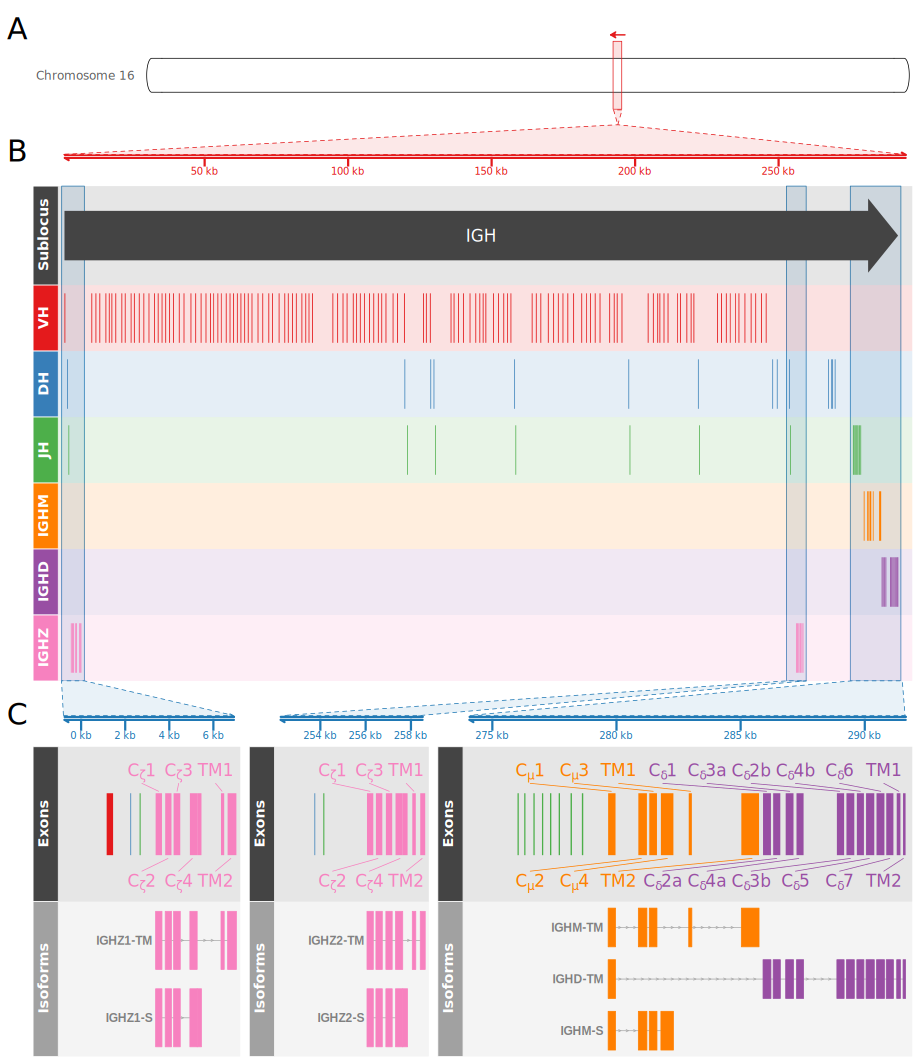
\includegraphics[width=\textwidth]{_Figures/png/xma-new-locus-map}
	\caption[The immunoglobulin heavy chain (\textit{IGH}) locus in \textit{}]{\textbf{The immunoglobulin heavy chain (\textit{IGH}) locus in \textit{Xiphophorus maculatus}:} (A) Position of the \textit{IGH} locus on chromosome (group) 16 of the \Xma genome. (B) Arrangement of \vh, \dh, \jh and constant-region gene segments on the \Xma \igh{} locus. (C) Detailed map of the \igh{Z1}, \igh{Z2} and \igh{M/D} constant regions, indicating the position and identity of the constant-region exons and the exon composition of expressed \igh{} isoforms in \Xma. Note change of orientation between subfigures (A) and (B-C).}
	\begin{subfigure}{0em}
        \phantomsubcaption{}
        \label{fig:xma-locus-map-a}
    \end{subfigure}
    \begin{subfigure}{0em}
        \phantomsubcaption{}
        \label{fig:xma-locus-map-b}
    \end{subfigure}
    \begin{subfigure}{0em}
        \phantomsubcaption{}
        \label{fig:xma-locus-map-c}
    \end{subfigure}
	\label{fig:xma-locus-map}
\end{figure} % TODO: Fix to remove IGHZ2-S

\begin{figure}
\centering
\includegraphics[width=\textwidth]{_Figures/png/species-tree-small}
\vspace{0.5em}
\caption[Summary of important \igh{} phenotypes in killifish, platyfish, and medaka]{\textbf{Summary of important \igh{} phenotypes in killifish, platyfish, and medaka:} Cladogram of the evolutionary relationship between southern platyfish (\xma), turquoise killifish (\nfu) and medaka (\species{Oryzias}{latipes}), with three-spined stickleback (\species{Gasterosteus}{aculeatus}) as an outgroup. The state of various \igh{} phenotypes of interest are annotated to the right of the tree; states deviating from the expected teleost configuration are in bold.}
\label{fig:species-tree-small}
\end{figure}
	
\subsection{Constant regions}
\label{sec:xma-locus-constant}
	
As discussed briefly in \Cref{sec:xma-locus-structure}, the \Xma \igh{} locus contains two distinct \igh{Z} constant regions: one in the usual position immediately preceding the \igh{M}-associated D- and J-regions, the other, unexpectedly, at the far 5'-extremity of the locus (\Cref{fig:xma-locus-map-b}). Both \igh{Z} constant regions occupy the expected configuration, with four \cz{} exons, two transmembrane exons, and a secretory tail (\Cref{fig:xma-locus-map-c}, \Cref{tab:xma-ch-coords}). However, in contrast to the duplicate constant regions in \Nfu, the two \igh{Z} constant regions in \Xma are quite distinct from each other in sequence, with an average of only \pc{64} nucleotide and \pc{48} amino-acid sequence identity between corresponding \cz{} exons (\Cref{fig:xma-cz-aln}, \Cref{tab:xma-cz-aln}). This unexpectedly high level of sequence divergence suggests a relatively ancient duplication event, and raises the possibility that the lineage giving rise to \Nfu may have lost not one, but two distinct \igh{Z} constant regions.
	
\begin{table}
	\centering
	\caption[Sequence similarity between \igh{Z} constant-regions in \Xma]{\textbf{Sequence similarity between \igh{Z} constant-regions in \Xma:} Percentage sequence identities of pairwise Needleman-Wunsch global alignments between nucleotide (NT) or amino-acid (AA) sequences of corresponding \cz{} exons from the two \igh{Z} constant regions of \Xma \textit{IGH}.}
	% latex table generated in R 3.5.2 by xtable 1.8-3 package
% Tue Jan 15 19:07:19 2019
\begin{tabular}{llrr}
  \toprule Isotype & Exon & NT & AA \\ 
  \midrule Z & 1 & 59.14 & 44.57 \\ 
  Z & 2 & 63.93 & 53.41 \\ 
  Z & 3 & 66.19 & 43.48 \\ 
  Z & 4 & 65.15 & 50.49 \\ 
   \bottomrule \end{tabular}

	\label{tab:xma-cz-aln}
\end{table}

While the state of \igh{Z} constant regions differs markedly between \Xma and \Nfu, the configurations of the \igh{M} and \igh{D} constant regions of the two species are quite similar, with a {\cm{1}-\cm{2}-\cm{3}-\cm{4}-TM1-TM2} configuration for \igh{M} and a {\cd{1}-(\cd{2}-\cd{3}-\cd{4})$_2$-\cd{5}-\cd{6}-\cd{7}-TM1-TM2} configuration for \igh{D} (\Cref{fig:xma-locus-map-b,fig:xma-locus-map-c}, \Cref{tab:xma-ch-coords}). In the \Xma locus, these constant regions and \igh{Z1} adopt the standard configuration seen in comparatively simple teleost \igh{} loci like those of zebrafish and fugu, with a {\vh-\dh-\jh-\textbf{CZ}-\dh-\jh-\textbaf{CM}-\textbf{CD}} arrangement that allows the choice between \igh{Z} and \igh{M/D} usage to be made via the choice of \dh segment during VDJ-recombination. However, whether such a mechanism is also responsible for the choice between these constant regions and \igh{Z1}, which lies more than \kb{200} away and upstream of the great majority of \vh segments in the locus (\Cref{sec:xma-locus-variable}) is questionable.

In order to investigate the expressed isoforms present in \Xma, published RNA-sequencing reads from various platyfish tissues (BioProject accession PRJNA420092, all libraries). were aligned together to the \igh{Z} and \igh{M/D} constant regions with \program{STAR}. The results indicate the expected six-exon transmembrane configuration in both \igh{Z1} and \igh{Z2}, as well as a secretory form of \igh{Z1} comprising \cz{1} to \cz{4} plus a \bp{23} secretory tail formed by a transcriptional run-on event from \cz{4} (\Cref{fig:xma-locus-sashimi-z1,fig:xma-locus-sashimi-z2}). However, while an in-frame secretory tail of similar length (\bp{20}) can be found in \igh{Z2}, it does not appear to be expressed in the read sets analysed here, indicating that \igh{Z2} may only be expressed in transmembrane form in the individuals sampled (\Cref{fig:xma-locus-sashimi-z2}).

Meanwhile, the results for \igh{D} (\Cref{fig:xma-locus-sashimi-d}) indicate a similar configuration to that observed in turquoise killifish, with a chimeric \cm{1} followed by 10 \cd{} exons and two transmembrane exons; as in \Nfu, neither a dedicated \igh{D} secretory exon nor a post-\cd{7} secretory tail was identified, suggesting that \igh{D} may be produced solely in transmembrane form in this species. Secretory \igh{M} (\igh{M-S}) was also found to occupy the same four-exon configuration seen in turquoise killifish and elsewhere. However, the configuration observed for transmembrane \igh{M} (\igh{M-TM}) did not correspond to the four-exon structure shared between turquoise killifish and medaka (\Cref{fig:nfu-locus-sashimi-a}); rather, \igh{M-TM} in \Xma occupies the five-exon configuration seen in most characterised teleosts (\Cref{fig:teleost-igm-exons-d}). This surprising difference indicates that two different splice configurations of \igh{M-TM} persist in the cyprinodontiform lineage, and raises the question of what, if any, functional difference arises from the presence or absence of \cm{3} in transmembrane \igh{M} in different species. However, it remains unclear whether this pattern of exon usage (\Cref{fig:species-tree-small}) is the result of independent changes in medaka and turquoise killifish or of a reversion in \Xma to the primitive teleost configuration.
	
\begin{figure}
	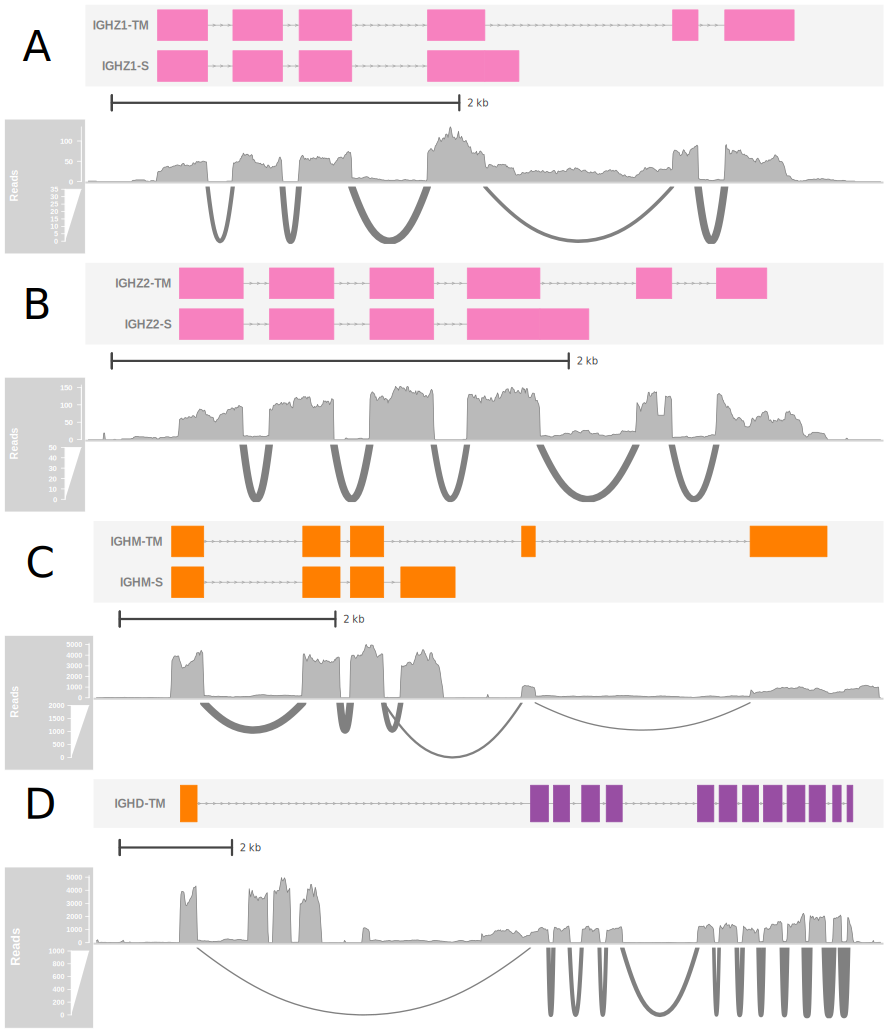
\includegraphics[width=\textwidth]{_Figures/png/xma-new-locus-sashimi}
	    \begin{subfigure}{0em}
        \phantomsubcaption{}
        \label{fig:xma-locus-sashimi-z1}
    \end{subfigure}
    \begin{subfigure}{0em}
        \phantomsubcaption{}
        \label{fig:xma-locus-sashimi-z2}
    \end{subfigure}
	\begin{subfigure}{0em}
        \phantomsubcaption{}
        \label{fig:xma-locus-sashimi-m}
    \end{subfigure}
    \begin{subfigure}{0em}
        \phantomsubcaption{}
        \label{fig:xma-locus-sashimi-d}
    \end{subfigure}
	\caption[Constant-region isoforms in \Xma]{\textbf{Constant-region isoforms in \Xma:} Coverage and sashimi plots of STAR-aligned RNA-seq reads from \Xma samples, demonstrating the splicing behaviour of \igh{} constant-region isoforms. (A) \igh{Z1} exon splicing, showing alternative use of the \cz{4}/TM1 splice junction and the post-\cz{4} secretory tail; (B) \igh{Z2} exon splicing; (C) IGHM exon splicing, showing alternative splicing patterns of IGHM-TM and IGHM-S; (D) IGHD exon splicing, including splicing of \cm{1} to \cd{1}.}
	\label{fig:xma-locus-sashimi}
	\end{figure}

	
\subsection{Variable regions}
\label{sec:xma-locus-variable}

In total, 125 \vh segments, 14 \dh segments and 15 \jh segments were identified in the \Xma IGH locus (\Cref{fig:xma-locus-map-b}). Of these, exactly one \vh (\igh{V01-01}), \dh (\igh{DZ01}) and \jh (\igh{JZ01}) lie upstream of the \igh{Z1} constant region, indicating that the variable-region sequence diversity available to this isotype is limited to a single VDJ combination. In contrast, the variable region between the end of \igh{Z1} and the start of \igh{Z2} is highly expanded, with 124 tightly-clustered \vh segments -- more than five times the total number seen in \Nfu, and more than seven times the number in the largest \Nfu sublocus. Of these 124 \vh segments, 106 (\pc{86}) are apparently functional, with the remainder pseudogenised by a variety of frameshift mutations, nonsense mutations, or truncation events (\Cref{tab:xma-vh-coords-1,tab:xma-vh-coords-2,tab:xma-vh-coords-3,tab:xma-vh-coords-4,tab:xma-vh-coords-5}); it remains to be seen whether \igh{V01-01} is also capable of recombining with \dh segments downstream of the \igh{Z1} constant region, and so constitutes part of the range of VDJ combinations available to the other constant regions. The \vh sequences in the \Xma locus are much more tightly packed than in the \Nfu locus, consistent with a lower overall prevalence of repetitive regions (21\%) in the \Xma genome \parencite{yuan2018repeats}.
	
In total, the \vh regions in \Xma \textit{IGH} fall into 23 families, of which eight contain multiple segments (\Cref{fig:xma-vh-families-tree,fig:xma-vh-families-map}); strikingly, the single \vh segment serving IGHZ (\igh{V01-01}) represents a separate family which is distinct from any other segment in the locus. To further investigate the evolutionary history of these families, the \vh segments from both the \Xma and \Nfu \igh{} loci were aligned together with \program{PRANK}, and the resulting alignment was used to construct a phylogenetic tree with \program{RAxML} \parencite{stamatakis2014raxml8,stamatakis2005raxml3,stamatakis2006raxml6}; the resulting tree (\Cref{fig:nfu-xma-vh-tree-nt}) revealed a clear interrelationship between the largest families in both loci (\Xma V02 and \Nfu V1), with a similar relationship observed for the second-largest families (\Xma V03 and \Nfu V2). 
In accordance with the close sequence relationship noted in \Cref{sec:nfu-locus-variable}, \Nfu V4 falls comfortably within the V03/V2 subtree, supporting its status as a pseudogenised subfamily of \Nfu V2.
		
In addition to its highly expanded \vh region, the variable region of the \Xma locus is unusual in the arrangement of its \dh and \jh segments (\Cref{tab:xma-dh-coords-seg,tab:xma-jh-coords-seg}): in addition to the relatively densely-packed blocks of four \dh and eight \jh regions between \igh{Z1} and \igh{M}, and the smaller groups of three \dh segments and one \jh segment between the last \vh segment and \igh{Z1}, small numbers of \dh and \jh segments are interspersed between blocks of \vh segments in the extended V-region between \igh{Z1} and \igh{Z2} (\Cref{fig:xma-locus-map-b}). Many of these segments are arranged such that groups of one or two \dh segments are closely associated with a single \jh segment, raising the possibility of a more cluster-like behaviour in which each VDJ group acts as a distinct recombination unit. However, the presence of larger D- and J-regions more closely upstream of the constant regions suggests a more conventional translocon behaviour; it remains to be seen which of these traditional models of antigen-receptor structure more closely matches the \textit{in vivo} recombination behaviour of this locus.
		
Finally, as is the case with \Nfu, the recombination signal sequences (RSSs) in \Xma IGH correspond closely to the standard expectations across the vertebrates, with the expected heptamer and nonamer consensus sequences and spacer length distributions (\Cref{fig:xma-rss-seqlogo-all,fig:xma-rss-seqlogo-sep}, 97.6\% of RSS spacers within \bp{1} of the expected conserved length).	

	\begin{figure}
		\begin{subfigure}{0em}
        \phantomsubcaption{}
        \label{fig:xma-rss-seqlogo-all-heptamer}
    \end{subfigure}
    \begin{subfigure}{0em}
        \phantomsubcaption{}
        \label{fig:xma-rss-seqlogo-all-spacer}
    \end{subfigure}
    \begin{subfigure}{0em}
        \phantomsubcaption{}
        \label{fig:xma-rss-seqlogo-all-nonamer}
    \end{subfigure}
	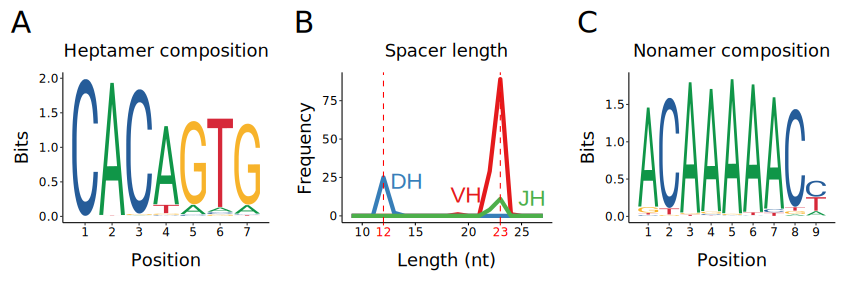
\includegraphics[width=\textwidth]{_Figures/png/xma-new-rss-seqlogo-all}
	\caption[Recombination signal sequences in the \Xma \textit{IGH} locus]{\textbf{Recombination signal sequences in the \Xma \textit{IGH} locus:} (A) Sequence composition of conserved heptamer sequences across all \Xma heavy-chain RSSs; (B) length distribution of unconserved spacer sequences in \Xma heavy-chain RSSs; (C) sequence composition of conserved heptamer sequences across all \Xma heavy-chain RSSs.}
	\label{fig:xma-rss-seqlogo-all}
	\vspace{1em}
	\end{figure}

	
	\begin{figure}
	\centering
	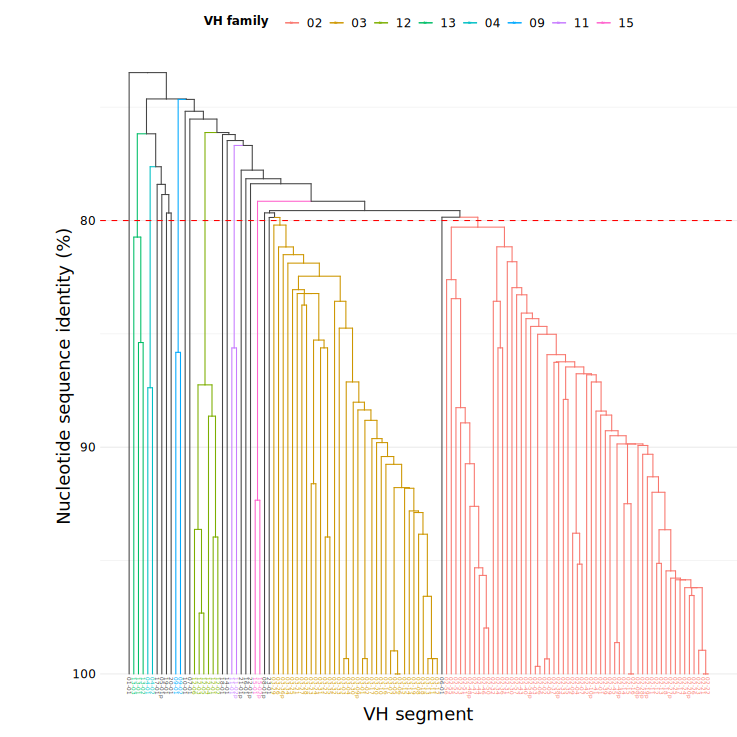
\includegraphics[width=\textwidth]{_Figures/png/xma-vh-families-tree}
	\caption[Dendrogram of \vh families in the in \Xma \textit{IgH} locus]{\textbf{Dendrogram of \vh families in the in \Xma (\textit{IgH}) locus:} Dendrogram of sequence similarity of \vh segments in the \Xma locus, arranged by single-linkage clustering on nucleotide sequence identity. The red line indicates the 80\% cutoff point for family assignment, while branch colour indicates family membership:  \vh families containing multiple segments are uniquely coloured, while single-segment families are in grey.}
	\label{fig:xma-vh-families-tree}
	\end{figure}
		
	\begin{figure}
	\centering
	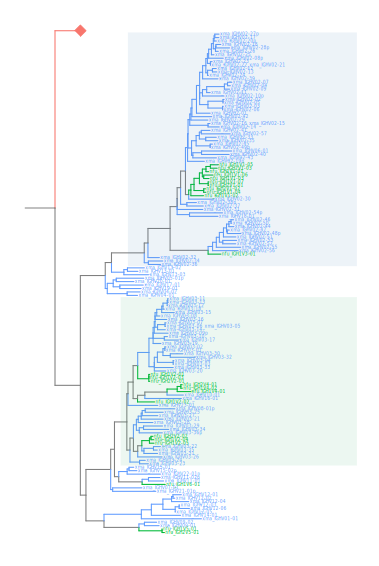
\includegraphics[width=0.8\textwidth]{_Figures/png/nfu-xma-vh-tree-nt.png}
	\caption[Evolutionary relationships between \vh families in \Xma and \Nfu]{\textbf{Evolutionary relationships between \vh families in \Xma and \Nfu:} Phylogenetic tree of evolutionary relationships between \textit{IGH} \vh segments in \Nfu and \Xma, as inferred from the nucleotide sequences of \vh segments from both loci. Note the close interrelationship between the largest (blue zone) and second-largest (green zone) families in each species. The red diamond indicates the location of the outgroup, which is composed of zebrafish \textit{TRB} V-segments.}
	\label{fig:nfu-xma-vh-tree-nt}
	\end{figure}
		
\FloatBarrier

\clearpage

%%%%%%%%%%%%%%%%%%%%%%%%%%%%%%%%%%%%%%%%%%%%%%%%%%%%%%%%%%%%%%%%%%%%%%%%%%%%%%%
% COMPARATIVE SECTION
%%%%%%%%%%%%%%%%%%%%%%%%%%%%%%%%%%%%%%%%%%%%%%%%%%%%%%%%%%%%%%%%%%%%%%%%%%%%%%%


\section{\igh{} constant-region evolution in the Cyprinodontiformes}
\label{sec:comparative}

The characterised \igh{} loci of \nfu, \xma and medaka together reveal a high degree of variability in structure and function across the atherinomorph clade, with ... .


Many of these 

In this section, I address two of the most interesting of these questions, in particular the evolutionary history of 
	
In this section, I trace the evolutionary history of ...
	
In order to address these questions, I identified and analysed the \igh{} constant-regions present in a further ten cyprinodontiform species (\Cref{fig:species-tree-large-taxa}, \dots), % TODO: Table of analysed species and genomes
as well as a new and improved genome assembly of medaka (\dots), % TODO: Cite genome accession
using the same methods described for \Nfu and \Xma (\dots). % TODO: Cite methods description, describe manual refinement methods
Where possible, the indentified exons were then grouped by order and spatial proximity to identify contiguous constant-regions, enabling the presence/absence and number of constant regions of each isotype to be estimated for each species. % TODO: Table for this
Finally, the \cm{}, \cd{} and \cz{} exons so identified, along with those of \Nfu and \Xma identified in \Cref{sec:nfu-locus} and \Cref{sec:xma-locus}, were used to construct a large multiple-sequence alignment with \program{PRANK}, which was in turn used to build a phylogenetic tree of \ch{}-exon evolution in the Atherinomorpha.

 aligned with \program{PRANK}, and the resulting multiple-sequence alignment was used to build a phylogenetic tree of \ch-exon evolution 
 
 \begin{figure}
	\centering
	\includegraphics[width=0.9\textwidth]{_Figures/png/cyprinodontiform-ch-tree}
	\caption[\igh{Z} in the Atherinomorpha has been lost multiple times independently]{\textbf{\ch exons } Unrooted phylogram of \ch exons in \dots. %TODO: Denote species
	Each exon type is clustered separately in the tree topology and has been highlighted and labelled accordingly.}
	\label{fig:cyprinodontiform-ch-tree}
\end{figure} % TODO: Update tree


	\subsection{Evolutionary history of IgZ} % TODO: Better title
	
	The specialised mucosal isotype \igh{Z} is present in the majority of teleost \igh{} loci characterised so far, including several species (including stickleback and fugu) relatively closely related to the Atherinomorpha; the possession of \igh{Z} therefore appears to be primitive to most groups of teleost fish. The striking absence of the isotype in both medaka and turquoise killifish (\Cref{sec:nfu-locus-constant}), the first two characterised \igh{} loci from the Atherinomorpha, suggested that the lack of \igh{Z} may have occurred in the common ancestor of both species and so be primitive both the Beloniformes and Cyprinodontiformes; however, the surprising presence of two distinct \igh{Z} loci in the locus of the southern platyfish \xma convincingly falsified this hypothesis and indicated that the loss of \igh{Z} in medaka and turquoise killifish occurred independently in their respective lineages (\Cref{sec:xma-locus-constant}). 
	
	To further investigate the distribution and evolutionary history of \igh{Z} in the Cyprinodontiformes, \igh{Z} exons from zebrafish, stickleback and \Xma were aligned to the genomes of ten additional cyprinodontiform species (\dots) % TODO: Table of species
with \program{BLAST}, and the resulting alignments were processed as described in \dots % TODO: methods ref
to obtain complete exon sequences. This process revealed the presence of complete \igh{Z} constant regions (defined as \cz{1}-\cz{2}-\cz{3}-\cz{4}-TM1)% ; TM2 exons were not identified in most species due to the extreme shortness of their coding sequence) in 
in seven of the ten new species in addition to \Xma, including several species intermediate between \Xma and \Nfu (\Cref{fig:species-tree-large-ighz}) -- confirming that \igh{Z} is present in multiple cyprinodontiform species and that its absence in medaka and turquoise killifish most likely arose via multiple independent deletion events. Furthermore, only a single pseudogenised transmembrane exon (without accompanying \cz{} exons) could be found in the genome of \species{Austrofundulus limnaeus}, suggesting that functional \igh{Z} may also be absent in this species; if this is the case, it would represent a third independent loss event within the Atherinomorpha.

\begin{figure}
	\centering
	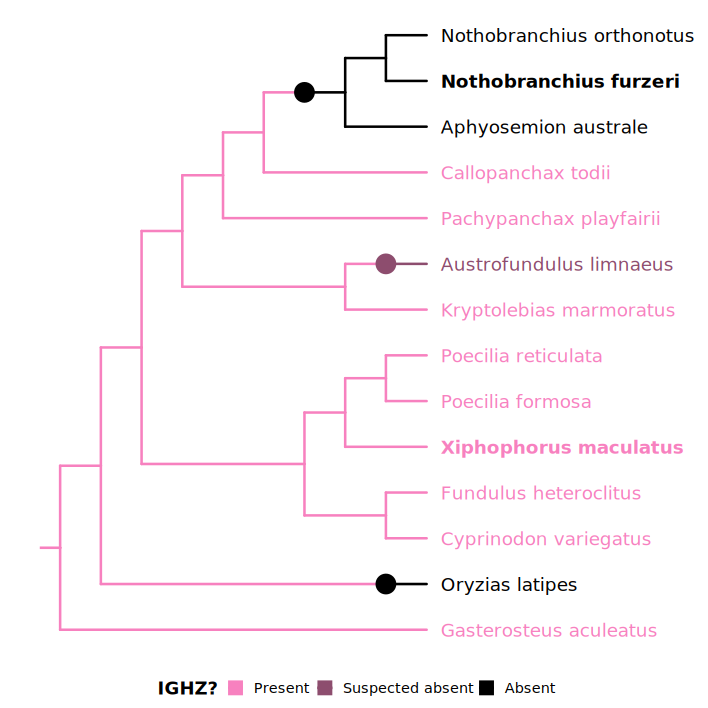
\includegraphics[width=0.9\textwidth]{_Figures/png/species-tree-large-ighz}
	\caption[\igh{Z} in the Atherinomorpha has been lost multiple times independently]{\textbf{\igh{Z} in the Atherinomorpha has been lost multiple times independently:} Cladogram of species reproduced from \Cref{fig:species-tree-large-taxa}, annotated according to the known (tip nodes) or hypothesised (internal nodes) presence or absence of intact \igh{Z} constant regions in each species. Large coloured points on the cladogram denote sites of hypothesised state changes; \igh{Z} is assumed to be primitively present in the clade and losses to be irreversible. The currently-available genome assembly of \textit{A. limnaeus} (purple) contains one pseudogenised \igh{Z-TM1} exon and no \cz{} exons.}
	\label{fig:species-tree-large-ighz}
\end{figure}

The \Xma \igh{} locus contains two distinct \igh{Z} constant regions, with only limited mutual sequence identity. % TODO: Ref figure and/or table here
Several other analysed species, including \dots, % TODO: species here
also exhibited multiple distinct \igh{Z} constant regions, suggesting a more complex pattern of \igh{Z} duplication and deletion than can be captured by a simple presence/absence metric. In order to better investigate the evolutionary history of \igh{Z} constant regions in the Cyprinodontiformes, the \cz{1}--\cz{4} nucleotide sequences of each observed constant region were concatenated together, aligned with \program{PRANK} and used to construct a phylogenetic tree with \program{RAxML}. 

The resulting tree (\Cref{fig:multispecies-cz-tree}) reveals three distinct lineages of \igh{Z} constant regions within the Cyprinodontiformes, each of which is present in multiple different species. Two of these, lineage A and B, correspond to \Xma \ighz{1} and \ighz{2}, respectively, while a third lineage C is represented in a close relative of \Xma (\species{Poecilia formosa}, the Amazon molly) but not \Xma itself. 

\begin{figure}
	\centering
	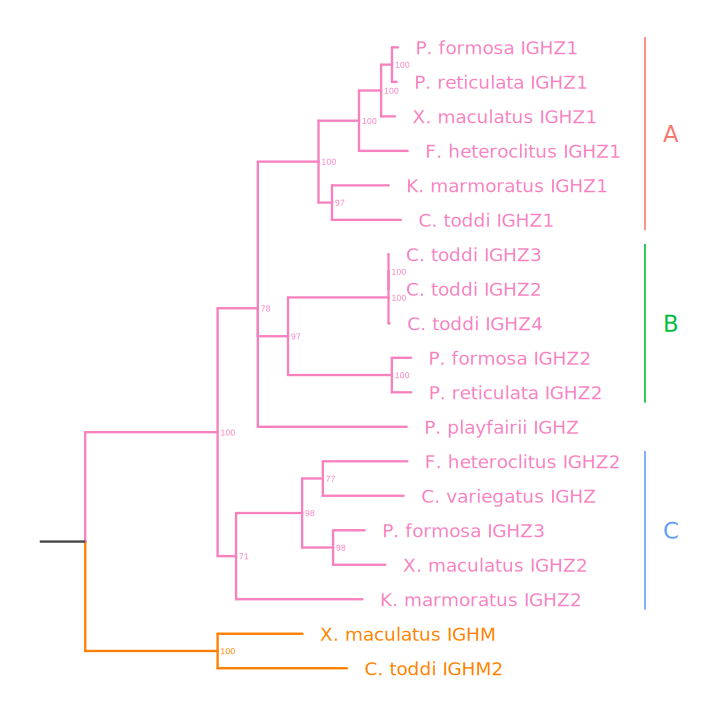
\includegraphics[width=0.9\textwidth]{_Figures/png/multispecies-cz-tree}
	\caption[\igh{Z} in the Atherinomorpha has been lost multiple times independently]{\textbf{\igh{Z} in the Atherinomorpha has been lost multiple times independently:} 
	Phylogram of concatenated \cz{1}--\cz{4} nucleotide sequences from \igh{Z}-bearing species from \dots % TODO: Designate species
	, with }
	\label{fig:multispecies-cz-tree}
\end{figure}

Only one \igh{Z} constant region from the analysed species could not be confidently assigned to one of these three lineages, namely the single \igh{Z} of \species{Pachypanchax playfairii}. In order to more closely investigate the relationships of \igh{Z} in this species, the exon sequences of \species{P. playfairii} \cz{1}--\cz{4} were separately aligned to the \cz{} exons of all other \igh{Z}-bearing species using Needleman-Wunsch global alignments, and the distribution of alignment scores was plotted in \dots % Figure
. The results show a striking difference in alignment behaviour between the exons, with \cz{1} and \cz{2} clearly aligning to exons from the B lineage and \cz{3} and \cz{4} showing more ambiguous affinity for either A- or C-lineage sequences. This unexpected behaviour suggests that the \species{P. playfairii} \igh{Z} sequence may be the result of a deletion or fusion event combining the first two exons of a B-lineage \igh{Z} constant region with the latter exons of a constant region from another lineage, resulting in a chimeric gene with ambiguous ancestry.

In summary, the cyprinodontiforms ancestrally possessed at least three variants of \igh{Z}, giving rise to multiple lineages of \igh{Z} constant regions evolving in parallel across the clade. Each of these lineages appears to have been lost in multiple cyprinodontiform species, with different species showing distinct patterns of retention and loss, and in at least one lineage -- that of \species{Pachypanchax playfairii} -- two different \igh{Z} lineages have fused to produce a chimeric isotype. All three lineages are missing from a subset of species in the Nothobranchiidae (including \nfu), and also appear to have been independently lost in \species{Austrofundulus limnaeus}. Taken together, these data suggest a high degree of complexity and volatility in the evolution of mucosal adaptive immunity in the Cyprinodontiformes.
	
	
	
	
	
	\subsection{Sublocus multiplicity and orientation}
	
	\subsection{Exon usage in transmembrane IgM \& other isoforms}


	%	The examination of the constant-region structures present in the \Xma IGH locus therefore reveals three notable features that differ in state between medaka, turquoise killifish, and the southern platyfish. Most strikingly, the absence of IGHM in medaka and killifish, but its presence in platyfish, strongly suggests that the isoform has been lost independently in the two groups. Conversely, the presence of a four-exon IGHM-TM in medaka and killifish, but a five-exon configuration in platyfish, is less clear-cut: it may indicate an independent change in medaka and killifish that is absent in platyfish, but may also plausibly represent a reversion in platyfish to the more-primitive five-exon state. Without a deeper understanding of the currently-unknown physical underpinnings of this observed difference in splicing behaviour, this question can only be addressed through analysis of RNA-seq data from a large number of related species, something beyond the scope of the present investigation. % TODO: Do it anyway?
%	Finally, the presence of a (\cd{2}-\cd{3}-\cd{4}) duplication in both platyfish and killifish, but not in medaka, suggests that this may be a shared primitive feature of the Cyprinodontiforms; however, given the apparent recurrence of this duplication pattern in many different groups across the teleosts, a strong conclusion cannot be drawn without a higher-resolution phylogenetic analysis of a larger number of related species. % TODO: See section ... etc.
% TODO: Move to multispecies section intro

	%	TODO: Move to multilocus section. Alongside this, I performed a more limited characterisation of the \textit{IgH} constant regions in 9 %?
%	additional cyprinodontiform and beloniform species, to assess the broader patterns of immunoglobulin heavy chain evolution within these groups (\Cref{sec:comparative-loci}). The results of these additional investigations repeatedly called into question the hypothesis of homology in IgH locus ideosyncracies between medaka and turquoise killifish, and suggest a model of rapid locus evolution within this diverse and important teleost clade.
	
	% TODO: Move to discussion section.
	% TODO: Relationship between killifish Vs and other species
	% TODO: Evolution of IGH1 vs 2
	% TODO: Discussion of mucosal immunity in absence of IGZ
		% TODO: Discuss smallness of killifish locus in the context of relaxed purifying selection and short life span
	% TODO: Section on "Investigating the evolutionary relationship between IGH1 and IGH2"
	% Keep for discussion:
%\q{Given the lack of IgZ in this species, how do you think they carry out mucosal immunity?}
%
%I'd assume using IgM. It's the primitive antibody and is expressed in secreted form in the killifish gut. I haven't investigated the protein expression so it's hard to say for sure, but I'd guess that's the answer. It's also quite possible, lacking a specialised mucosal class, that the answer is ``not very well". It would be very interesting to compare mucosal immune function in species with and without IgZ, especially if those species are closely related.
%
%Given the impressive results indicating the specificity of IgT for mucosal immunity in trout, and the lack of mucosal response of IgM in that species, it would be very interesting to see what mucosal responses look like in a species that lacks that isotype -- is IgM much more responsive and expressed in the gut than in IgT-possessing species, or is the mucosal response just worse?
	% (Incidentally, it would be great to see whether any B-cells in TK show recombinations in both subloci, vs one or the other. Single-cell DNA sequencing could plausibly do this.)








	



 
%!TEX root = ../thesis.tex
% TODO: Change this?

\chapter{Immunoglobulin sequencing in \textit{Nothobranchius furzeri}} 
\label{chap:igseq} 
\onehalfspacing
\pagebreak

\section{Introduction}
\label{sec:igseq_intro}

\dots

\section{Collecting killifish samples for immunoglobulin sequencing}
\label{sec:igseq_samples}

To obtain samples for establishing and validating an immunoglobulin-sequencing protocol in turquoise killifish, as well as to investigate changes in killifish repertoires with age, male GRZ-AD turquoise killifish from a single hatching cohort were raised under standard husbandry conditions (\Cref{sec:methods_husbandry}) and sacrificed by anaesthesia, followed by flash-freezing in liquid nitrogen and preservation at \degC{-80}. In total, thirty-two fish were sacrificed at four total time points (\Cref{tab:igseq-cohorts-summary,tab:igseq-cohorts-fish}): regular groups of ten fish each were sacrificed at roughly 5.5 weeks (shortly after reproductive maturation), 8 weeks (middle adulthood) and 10.5 weeks (close to median lifespan) post-hatching, while two surviving fish were sacrificed eight weeks later at roughly 18 weeks post-hatching.

\begin{table}
\caption{Summary of killifish used in \igseq validation and ageing experiment. All fish are GRZ-AD strain and male.}
\label{tab:igseq-cohorts-summary}
% latex table generated in R 3.5.2 by xtable 1.8-3 package
% Wed Jan 30 11:19:43 2019
\begin{tabular}{rrlllll}
  \toprule Group & \# Fish & Hatch date & Sacrifice date & Age (days) & Age (weeks) & Mean weight (g) \\ 
  \midrule 1 & 10 & 2016-05-09 & 2016-06-17 & 39 & 5.57 & 1.3 \\ 
  2 & 10 & 2016-05-09 & 2016-07-04 & 56 & 8 & 1.37 \\ 
  3 & 10 & 2016-05-09 & 2016-07-21 & 73 & 10.4 & 1.76 \\ 
  4 & 2 & 2016-05-09 & 2016-09-14 & 128 & 18.3 & 2.3 \\ 
   \bottomrule \end{tabular}

\end{table}

In order to obtain a representative sample of the whole-body antibody repertoires from these individuals (as opposed to the specific repertoire of a particular organ), the frozen fish were homogenised in liquid nitrogen with a mortar and pestle, and total RNA was isolated from the resulting powder with guanidinium thiocyanate-phenol-chloroform extraction (\Cref{sec:methods_molec_standard_qiazol}).

\section{\igseq in the turquoise killifish: principles and protocols}
\label{sec:igseq_protocol}

\subsection{Preparing the sequencing library}
\label{sec:igseq_protocol_library}

% TODO: Add general description of what IgSeq is and why you might do it (if not in introduction)

\IGSEQ is a precise and quantitative method which is highly sensitive to biases and errors arising during both library preparation (especially PCR) and sequencing. In order to minimise the impact of these errors on the results, unique molecular identifiers (UMIs) are widely used in \igseq library-preparation protocols to uniquely label each input molecule, enabling sequences in the dataset arising from the same input molecule to be identified, grouped and collapsed into a single consensus sequence. This process effectively corrects for biases in apparent abundance arising from differential amplification during library-preparation or differential clustering during sequencing, and allows identical sequences descended from the same input molecule to be distinguished from those descended from different input molecules with the same sequence \parencite{vollmers2013consensus}. In addition, as long as enough reads arising from a given input sequence are present, the taking of a consensus sequence from each UMI group effectively corrects for sequence errors arising during library-preparation and sequencing, enabling the original input sequence to be reconstructed much more accurately (\Cref{fig:umi-consensus-schema}) \parencite{vollmers2013consensus,turchaninova2016igprep}.

In the \igseq protocol established here for the turquoise killifish, the addition of UMIs is achieved through the use of a procedure adapted from \parencite{turchaninova2016igprep}. This procedure takes advantage of the intrinsic terminal transferase activity exhibited by reverse-transcriptase enzymes derived from Moloney Murine Leukemia Virus (MMLV), which includes most commercially-available reverse-transcriptase enzymes. Upon reaching the end of an RNA template, such viruses add a variable number of untemplated deoxyribonucleotides to the 3'-end of the new cDNA molecule, with a strong bias for cytidine residues \parencite{zajac2013switching}. If a template-switch adapter (TSA) oligonucleotide ending in riboguanosines is added to the reaction mixture, it will pair with these untemplated terminal cytidines to form a new priming site for the reverse transcriptase. The enzyme will then re-attach to this new priming site and process to the end of the paired oligo, adding the sequence of the TSA to the 3'-end of the cDNA \parencite{zajac2013switching}. This procedure, known as template switching (\Cref{fig:template-switch-schema}), enables semi-arbitrary sequences to be prepended to the reverse-transcribed mRNA sequence, including a primer sequence and (in this case) a UMI \parencite{turchaninova2016igprep}.

\begin{figure}
\centering
\includegraphics[width=0.7\textwidth]{_Figures/png_edited/umi-consensus-schema}
\caption{\textbf{Correcting errors and biases with unique molecular identifiers (UMIs):} In this simplified schematic, three template RNA molecules representing two distinct sequences (red and blue rectangles) are tagged with UMIs (coloured left-hand ends) prior to PCR-based library preparation and sequencing. As a result of differential amplification bias between the sequences, the less-abundant input sequence gives rise to a larger number of sequencing reads; however, by aligning and collapsing matching UMI groups into consensus reads, the original proportions of the sample can be reconstructed. Consensus-read generation also enables the correction of various PCR and sequencing errors (thin red/green bars), the majority of which are present in only a minority of sequence copies within a UMI group; only the dark-blue UMI group, for which only a single sequencing read was obtained, cannot be effectively corrected in this way.}
\label{fig:umi-consensus-schema}
\end{figure}

\begin{figure}
\centering
\includegraphics[width=0.7\textwidth]{_Figures/png_edited/template-switch-labelled}
\vspace{0.5em}
\caption{\textbf{Addition of a known 5'-sequence with template switching:} In this simplified schematic, an MMLV-derived reverse-transcriptase enzyme (blue oval) binds a primed RNA template and processes to the 5-prime end (A), where it deposits additional untemplated cytidine residues at the 3'-end of the CDNA (red bar) using its terminal-transferase activity (B). A template-switch adaptor (TSA) with complementary terminal guanosine residues (blue bar) pairs with these terminal cytidines (C), creating a new double-stranded priming site to which the reverse-transcriptase enzyme can bind (D). Processing of the enzyme to the end of the TSA sequence produces a cDNA molecule with an additional, known 3' sequence (E).}
\label{fig:template-switch-schema}
\end{figure}

In the library-preparation protocol used for \Igseq in the turquoise killifish, therefore, reverse-transcription is performed on total RNA using a gene-specific primer (GSP) homologous to the constant-region sequence of the isotype of interest and an MMLV-derived reverse-transcriptase enzyme optimised for its terminal-transferase activity (\Cref{sec:methods_molec_igseq_rt}). A template-switch adaptor containing a constant primer sequence and random UMI sequence (\Cref{fig:igseq-tsa-sequence}) is included in the reaction mixture and added to the cDNA sequence via template switching. In addition to enabling UMI-based clustering and correction as described above, this approach has the additional advantage of bypassing the variable region of the \igh{} transcript and thus avoiding the use of multiplexed V-segment primers, which may introduce additional biases through differential binding affinity between V-segments \parencite{rosati2017methods}.

\begin{figure}
\begin{center}
\LARGE
\textcolor{Fuchsia}{AAGCAGUGGTAUCAACGCAGAG}U\textcolor{ForestGreen}{NNNN}--\\--U\textcolor{ForestGreen}{NNNN}U\textcolor{ForestGreen}{NNNN}UCTT\textcolor{BurntOrange}{rGrGrGrG}
\end{center}
\caption{Annotated sequence of the SmartNNNa barcoded template-switch adapter (TSA) used in template-switch reverse-transcription for \igseq library preparation \parencite{turchaninova2016igprep}. The 5'-terminal purple characters represent a constant sequence used for primer-binding in downstream PCR steps, while the green N characters represent the random nucleotides used in the unique molecular identifier (UMI), each of which could take any value from A, C, G or T. The U residues represent deoxyuridine, which is specifically digested after reverse-transcription to remove residual TSA oligos from the reaction mixture (\Cref{sec:methods_molec_igseq_rt}). The orange, 3'-termial rG characters indicate riboguanosine residues, which pair with terminal-transferase-added cytidine residues during template switching.}
\label{fig:igseq-tsa-sequence}
\end{figure}

\begin{figure}
\centering
\caption{\textbf{Summary of \igseq library-preparation protocol}}
\label{fig:igrace-pipeline}
\includegraphics[width=0.7\textwidth]{_Figures/png_edited/igrace-pipeline-narrow}
\vspace{0.5em}
\end{figure}

Following reverse-transcription, the reaction mixture is treated with uracil-DNA glycosylase (UDG) to specifically remove residual TSAs through specific digestion of deoxyuridine residues (which are absent in the template sequence). The library then undergoes three successive rounds of PCR amplification (\Cref{fig:igrace-pipeline}; see\Cref{sec:methods_molec_igseq_pcr} for more details), which respectively serve to amplify the reverse-transcribed cDNA sequence; amplify further while adding partial Illumina TruSeq adaptor sequences; and add complete adaptor sequences including library-specific P1 and P2 index barcode sequences \parencite{vollmers2013consensus}. In the first two cases, the PCR primer sequences are homologous to the invariant part of the TSA sequence and the \cm{1} exon, respectively; as all known forms of \igh{} in turquoise killifish (\igh{M-TM}, \igh{M-S} and \igh{D-TM}) share this exon, the isotype- and isoform-specificity of the library prep can be altered simply by changing the position of the reverse-transcription GSP, with all other primer sequences left unchanged. In all experiments included in this chapter, a GSP on the \cm{2} exon was used, resulting in a library including \igh{M-TM} and \igh{M-S} sequences but excluding \igh{D}.

Libraries to be sequenced together are then pooled in equimolar ratio and the pooled sample undergoes size-selection to remove residual primer-dimers and other unwanted sequences. The complete library-preparation protocol reliably produces a single peak in the range of 650-\bp{680}, consistent with the known lengths of \vh, \dh and \jh gene segments in the \Nfu locus. % TODO: Figure for this, comparing expected and observed peak length
Following size-selection and quality control, pooled libraries are sequenced on an Illumina MiSeq sequencing machine with 2 × \bp{300} reads (\Cref{sec:methods_molec_igseq_seq}); this longer read length is necessary to completely cover the variable region. To avoid problems associated with the low sequence complexity of single-amplicon sequencing libraries, a large proportion of PhiX spike-in (30\%) was used to increase the sequence complexity of the libraries.

\subsection{Sequence pre-processing with \program{pRESTO}}
\label{sec:igseq_protocol_preprocess}

\begin{figure}
\centering
\caption{\textbf{Summary of \igseq pre-processing pipeline}}
\label{fig:igrace-preprocessing}
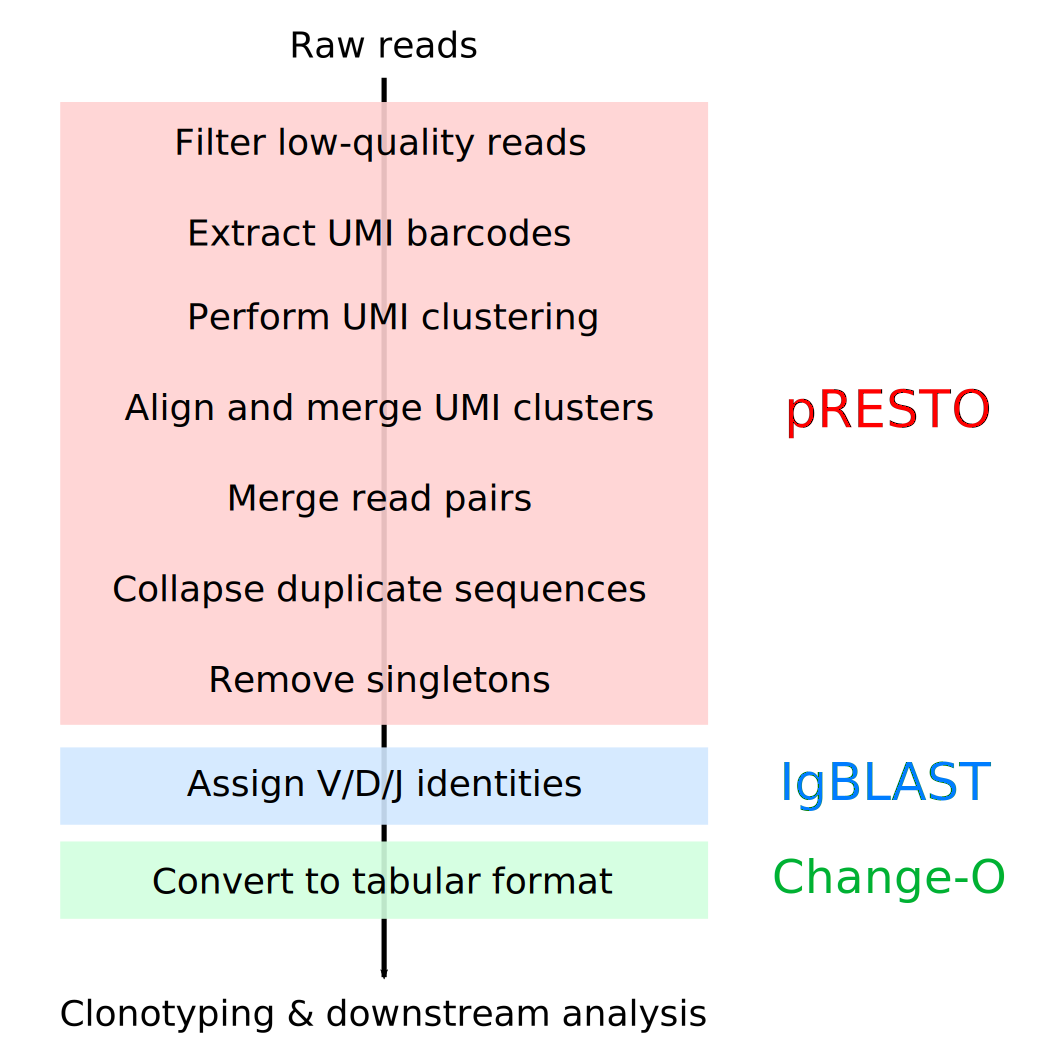
\includegraphics[width=0.6\textwidth]{_Figures/png_edited/igseq-preprocessing}
\vspace{0.5em}
\end{figure}

Raw \igseq data from the protocol described in \Cref{sec:igseq_protocol_library} takes the form of a large number of paired-end sequencing reads, each of which represents a partial, biased and error-prone sample from the set of input sequences in the original sample. To get from this fragmented and unreliable dataset to a set of complete, error-corrected and bias-adjusted \igh{} variable-region sequences, extensive pre-processing (\Cref{sec:methods_comp_igpreproc}) must be performed on the raw data. In this case, this pre-processing was largely carried out with \program{pRESTO} \parencite{vanderheiden2014presto}, part of the Immcantation suite of repertoire-sequencing analysis tools.

To begin with, each read pair in the dataset is annotated with various information about the source individual (ID, strain, sex, age and weight at death, etc.) as well as information about its place in the replicate structure of the experiment. The sequences are then filtered to remove low-quality sequences (with a mean Phred score of less than 20). % TODO: Citation for Phred score
Invariant primer sequences are trimmed from the ends of the reads, and the UMI sequence of each forward read (containing the TSA sequence) is extracted into a sequence annotation and removed from the read sequence.

As discussed in \Cref{sec:igseq_protocol_library}, the use of UMI sequences enables biases and errors in library insert sequences to be corrected by taking the consensus sequence of all reads sharing a given UMI. However, PCR and sequencing errors can also affect the sequence of the UMI itself, in which case reads that in fact belong to a single group will be spuriously separated during pre-processing; this can result in spuriously low UMI group sizes, spuriously high numbers of unique sequences, and avoidable loss of sequencing data due to reads with erroneous barcodes being discarded (as low-quality, low-read-count unique sequences) at various points in the pre-processing pipeline \parencite{shlemov2017igrec}. In addition to these barcode \textit{errors}, barcode \textit{collisions} can occur, in which multiple distinct sequences are labelled with the same UMI sequence and spuriously grouped together during UMI grouping. This can lead to spuriously large MIGs and spuriously low numbers of unique sequences, and in extreme cases lead to the rejection and loss of entire MIGs due to an insufficiently high level of sequence identity during consensus-read generation \parencite{shlemov2017igrec}.

In order to reduce the effect of such barcode errors and collisions on the pre-processing pipeline, primer-trimmed forward reads in this pipeline undergo clustering following extraction of UMI sequences. Firstly, reads are clustered by UMI sequence, and those with sufficiently similar UMIs are grouped together into a single cluster even if their UMIs differ slightly. Following this, read insert sequences within a given cluster are themselves clustered, and those with sufficiently different insert sequences are split apart into separate clusters. Following these clustering steps, each cluster consists of reads with highly similar barcode sequences as well as similar insert sequences; it is these clusters, rather than the raw UMI sequences, on which consensus-read generation is performed.

Following cluster inference as described above, annotations (including barcode and cluster annotations) are copied from each TSA-bearing forward-read to its mate among the reverse reads. The forward and reverse reads were then separately grouped by cluster identity and collapsed into a consensus sequence, based on the quality score of each aligned base call at each position \parencite{vanderheiden2014presto}. As most PCR and sequencing errors should be present in only a minority of the sequences descended from a given input sequence, this process effectively corrects these errors, while also removing the effect of biased amplification on observed sequence abundance. The more sequences present in a given cluster, the more effective is consensus-read generation at correcting these errors; as such, there is a trade-off inherent in the amount of oversequencing of the molecules in each library, with more oversequencing improving error correction but reducing the amount of data available \parencite{turchaninova2016igprep}.

Following consensus-read generation, pairs of forward and reverse consensus reads with matching cluster annotations are assembled into a single contiguous sequence, ideally covering the entire variable-region sequence of the template molecule; forward or reverse consensus reads lacking a mate in the other read set are discarded. At this point in the pipeline, each entry is assumed to represent a distinct RNA template molecule in the original sample. Sequences with different cluster annotations but matching insert sequences are then collapsed together into a single sequence, which is annotated with the number of contributing consensus reads; each sequence entry now represents a unique sequence in the dataset. Finally, unique sequences represented by only a single read pair (which could not be corrected by consensus-read generation and are therefore highly unreliable) are discarded.

At the end of the \program{pRESTO} pre-processing pipeline, the raw data has been processed into a set of complete variable-region sequences, each of which is annotated with the number of contributing reads and the number of distinct instances of that sequence found in the dataset. These sequences are then assigned V/D/J-identities through alignment to reference databases with \program{IgBLAST} \parencite{ye2013igblast}. Finally, the sequences and their metadata, including annotations and V/D/J-identities, are converted by \program{Change-O} (another program from the Immcantation suite) \parencite{gupta2015changeo} into tabular format for efficient downstream processing and analysis (\Cref{fig:igrace-preprocessing}).

\section{Establishing \igseq in turquoise killifish: pilot study}
\label{sec:igseq_pilot}

In order to refine and functionally validate the library-preparation protocol and processing pipeline described in \Cref{sec:igseq_protocol}, as well as assess the state of the turquoise-killifish antibody repertoire in mature adults, a group of four eight-week old adult male killifish from the second sample group described in \Cref{sec:igseq_samples} (specifically, fish 2-03, 2-04, 2-05 and 2-06 from \Cref{tab:igseq-cohorts-fish}) were selected for a pilot study. In this experiment, total RNA was isolated twice independently from each fish, and independent library preps were performed once on the first RNA isolate and twice on the second, for a total of three replicates per individual (\Cref{fig:igseq-pilot-design}). These twelve replicates were sequenced together in a single MiSeq run, yielding a total of \embed{_Figures/txt/pilot-reads-raw-total.txt} million read pairs (\embed{_Figures/txt/pilot-reads-raw-replicate-min.txt} to \embed{_Figures/txt/pilot-reads-raw-replicate-max.txt} million pairs per replicate, \embed{_Figures/txt/pilot-reads-raw-individual-min.txt} to \embed{_Figures/txt/pilot-reads-raw-individual-max.txt} million pairs per individual). These data were then used to develop the downstream analysis pipeline for killifish immunoglobulin-sequencing data, validate the performance and replicability of the protocol, and investigate the state of the antibody repertoire in mature adult killifish. % TODO: Cite appropriate subsections?

\begin{figure}
\centering
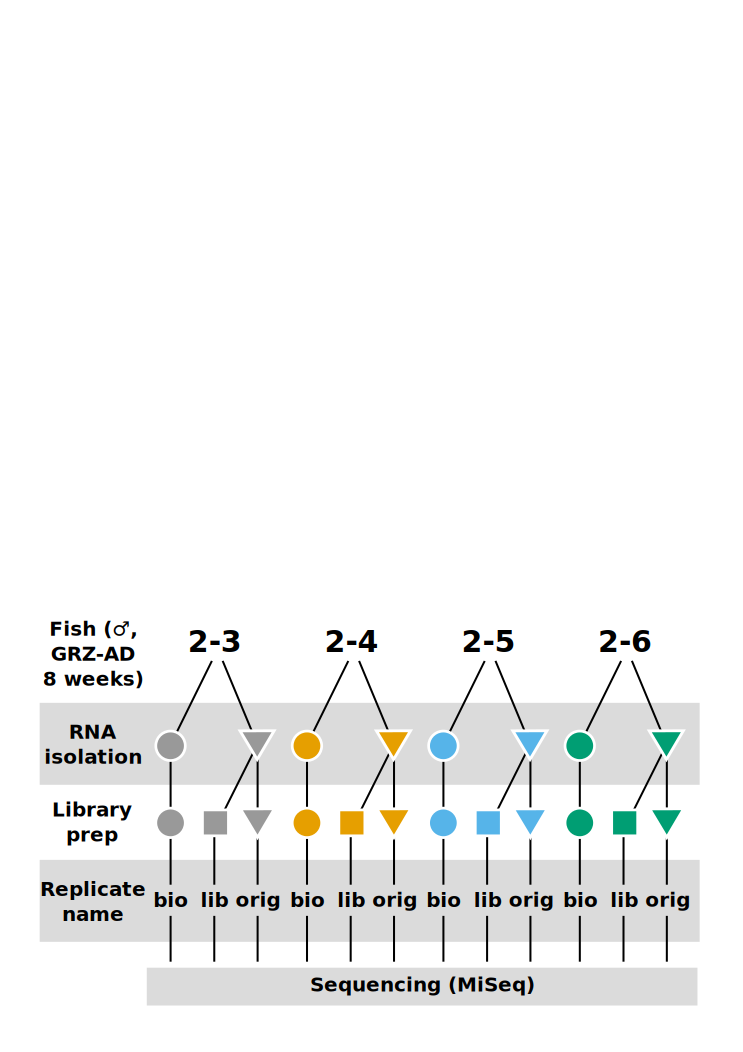
\includegraphics[width = 0.9\textwidth]{_Figures/png_edited/igseq-pilot-design_wide.png}
\caption{Experimental design of pilot study, showing relationship between replicates for each individual. Colour denotes individual of origin, while shape denotes replicate type.}
\label{fig:igseq-pilot-design}
\end{figure}

\subsection{Read survival and composition}
\label{sec:igseq_pilot_composition}

\Cref{fig:igseq-pilot-read-survival-init} shows the absolute and relative read survival for each of the twelve replicates throughout the pre-processing pipeline, up to and including VDJ assignment and Change-O table construction. The twelve replicates show relatively consistent behaviour, with \embed{_Figures/txt/pilot-read-survival-init-min.txt}\,\% to \embed{_Figures/txt/pilot-read-survival-init-max.txt}\,\% of reads surviving the entire process. Of those that do not, the biggest losses typically occur during quality filtering and removal of singleton sequences, with most other steps giving rise to relatively little sequence loss (\Cref{fig:igseq-pilot-read-survival-init-b}).

\begin{figure}
\centering
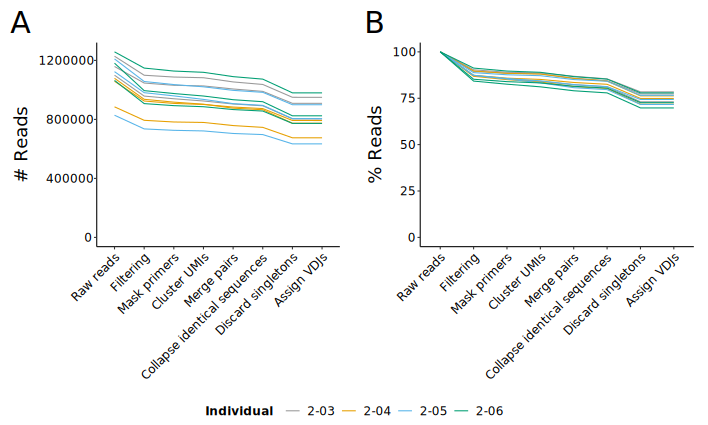
\includegraphics[width = 0.9\textwidth]{_Figures/png/pilot-read-survival-init.png}
\begin{subfigure}{0em}
\phantomsubcaption{}
\label{fig:igseq-pilot-read-survival-init-a}
\end{subfigure}
\begin{subfigure}{0em}
\phantomsubcaption{}
\label{fig:igseq-pilot-read-survival-init-b}
\end{subfigure}
\caption{Absolute (A) and relative (B) read survival during pre-processing of the pilot \igseq dataset, up to VDJ assignment and Change-O table construction.}
\label{fig:igseq-pilot-read-survival-init}
\end{figure}

In total, the pre-processed sequence repertoires of the pilot replicates contain between \embed{_Figures/txt/pilot-nseq-init-replicate-min.txt} and \embed{_Figures/txt/pilot-nseq-init-replicate-max.txt} unique sequences per replicate, corresponding to between \embed{_Figures/txt/pilot-nseq-init-individual-min.txt} and \embed{_Figures/txt/pilot-nseq-init-individual-max.txt} unique sequences per individual killifish and \embed{_Figures/txt/pilot-nseq-init-total.txt} unique sequences in total. Of these, \embed{_Figures/txt/pilot-nseq-init-pc-functional.txt}\,\% of sequences (corresponding to \embed{_Figures/txt/pilot-nreads-init-pc-functional.txt}\,\% of sequencing reads) are annotated by \program{Change-O} as functional, meaning they have successfully been assigned V- and J-identities, their V- and J-sequences are in-frame, and they do not contain any STOP codons (\Cref{fig:igseq-pilot-functional-prop-a}). A further \embed{_Figures/txt/pilot-nseq-init-pc-noj.txt}\,\% of sequences (corresponding to \embed{_Figures/txt/pilot-nreads-init-pc-noj.txt}\,\% of reads) failed to be assigned even an uncertain J-identity, meaning that no \jh sequence in the reference database aligned to the insert sequence; the remaining \embed{_Figures/txt/pilot-nseq-init-pc-other.txt}\,\% of sequences (corresponding to \embed{_Figures/txt/pilot-nreads-init-pc-other.txt}\,\% of reads) have a J-assignment but are rendered nonfunctional by an internal STOP codon and/or a frameshift between their V- and J-sequences (\Cref{fig:igseq-pilot-functional-prop-a}).

\begin{figure}
\centering
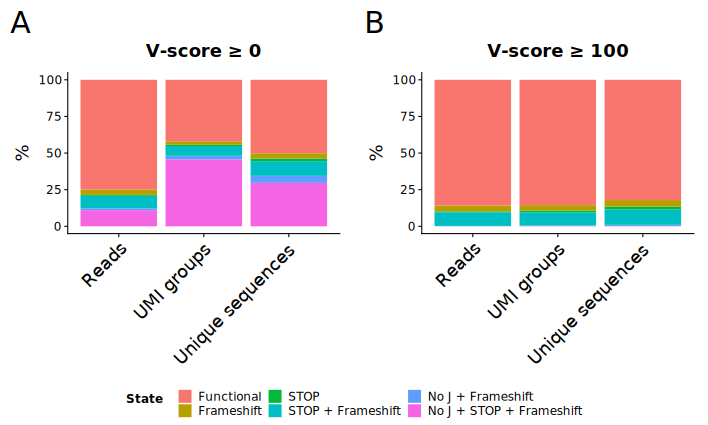
\includegraphics[width = 0.9\textwidth]{_Figures/png/pilot-functional-prop}
\begin{subfigure}{0em}
\phantomsubcaption{}
\label{fig:igseq-pilot-functional-prop-a}
\end{subfigure}
\begin{subfigure}{0em}
\phantomsubcaption{}
\label{fig:igseq-pilot-functional-prop-b}
\end{subfigure}
\caption{Proportion of input reads, UMI groups and unique sequences in the pilot \igseq dataset belonging to different (non)functional categories, before (A) and after (B) filtering on V-alignment score.}
\label{fig:igseq-pilot-functional-prop}
\end{figure}

As genuinely recombined but nonfunctional sequences would be expected to have undergone V(D)J recombination and so have a complete J-sequence, the lack of assigned J-identities for a significant minority of sequences suggests that this subset of sequences may be artefactual, erroneous or otherwise malformed. Supporting this assumption, sequences without J-assignments overwhelmingly have very low V-alignment scores reported by \program{IgBLAST}, with an average score of \embed{_Figures/txt/pilot-vscore-mean-noj.txt} $\pm$ \embed{_Figures/txt/pilot-vscore-sd-noj.txt} (mean $\pm$ standard deviation), compared to \embed{_Figures/txt/pilot-vscore-mean-other.txt} $\pm$ \embed{_Figures/txt/pilot-vscore-sd-other.txt} for other nonfunctional sequences and \embed{_Figures/txt/pilot-vscore-mean-functional.txt} $\pm$ \embed{_Figures/txt/pilot-vscore-sd-functional.txt} for functional sequences (\Cref{fig:igseq-pilot-functional-vscores}). A simple V-score cut-off of 100, therefore, effectively removes the vast majority of these low-quality sequences, while leaving the population of functional sequences intact (\Cref{fig:igseq-pilot-functional-prop-b}).

\begin{figure}
\centering
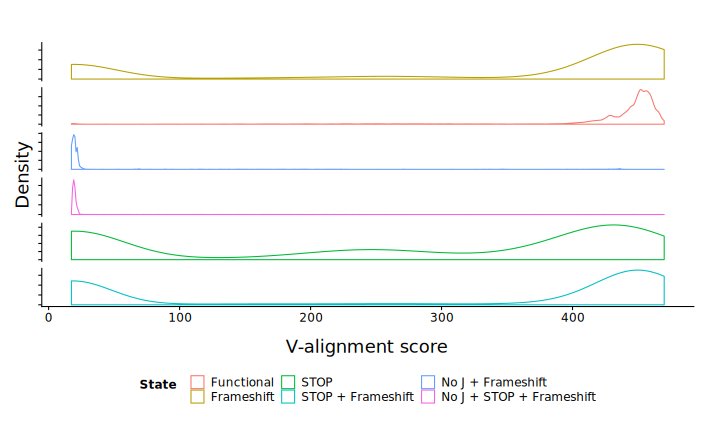
\includegraphics[width = 0.9\textwidth]{_Figures/png/pilot-functional-vscores}
\caption{Kernel density plots of distributions of V-alignment scores among unique sequences in the pilot \igseq dataset. Vertical axes are not to scale between sequence categories.}
\label{fig:igseq-pilot-functional-vscores}
\end{figure}

In total, \embed{_Figures/txt/pilot-nseq-init-dropped-vscore.txt} unique sequences, corresponding to \embed{_Figures/txt/pilot-read-survival-rel-loss-total.txt}\,\% of input reads, were removed in this way. As a result, including this final filtering step, between \embed{_Figures/txt/pilot-read-survival-all-min.txt}\,\% and \embed{_Figures/txt/pilot-read-survival-all-max.txt}\,\% of reads per input library survived the complete pre-processing process (\Cref{fig:igseq-pilot-read-survival-all}), a good range suggesting both that the library-preparation protocol successfully captured antibody-repertoire sequencing data from turquoise killifish for the first time, and that the subsequent computational pipeline was able to completely and successfully process the majority of the resulting data. Of the remaining \embed{_Figures/txt/pilot-nseq-init-kept-vscore.txt} unique sequences present in the dataset, \embed{_Figures/txt/pilot-nseq-init-functional-filtered.txt} (\embed{_Figures/txt/pilot-nseq-init-pc-functional-filtered.txt}\,\%) are functional, \embed{_Figures/txt/pilot-nseq-init-other-filtered.txt} (\embed{_Figures/txt/pilot-nseq-init-pc-other-filtered.txt}\,\%) are rendered nonfunctional by a STOP codon or frameshift, and only \embed{_Figures/txt/pilot-nseq-init-noj-filtered.txt} (\embed{_Figures/txt/pilot-nseq-init-pc-noj-filtered.txt}\,\%) could not be assigned a J-identity (\Cref{fig:igseq-pilot-functional-prop-b}). These results confirm that the data from this first \igseq experiment in the turquoise killifish are of sufficient quality to proceed to clonotyping and analysis of repertoire diversity.

\begin{figure}
\centering
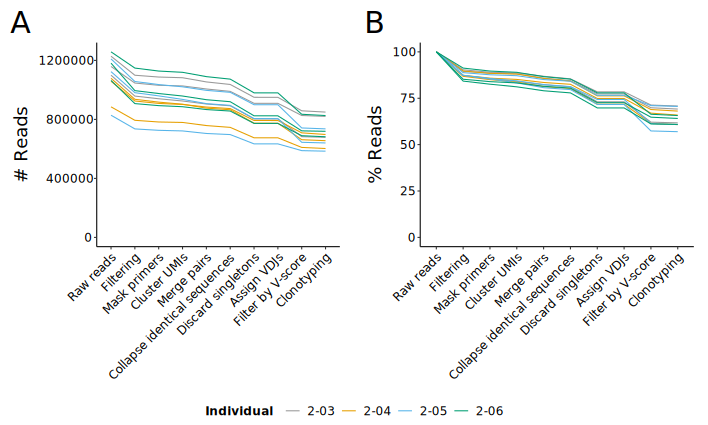
\includegraphics[width = 0.9\textwidth]{_Figures/png/pilot-read-survival-all.png}
\begin{subfigure}{0em}
\phantomsubcaption{}
\label{fig:igseq-pilot-read-survival-all-a}
\end{subfigure}
\begin{subfigure}{0em}
\phantomsubcaption{}
\label{fig:igseq-pilot-read-survival-all-b}
\end{subfigure}
\caption{Absolute (A) and relative (B) read survival during pre-processing of the pilot \igseq dataset, up to and including clonotyping.}
\label{fig:igseq-pilot-read-survival-all}
\end{figure}

\subsection{Clonotyping and clonal repertoire diversity}
\label{sec:igseq_pilot_clones}

Following assignment of VDJ identities and quality filtering, sequences in an antibody repertoire can be assigned to clones: groups of B-cells descended from a single \naive B-cell ancestor, and therefore sharing a single VDJ-recombination event. Sequences in the same clone are said to share a \textit{clonotype}. In \program{Change-O}, clonotyping is performed by dividing sequences into groups sharing a consistent V-assignment, J-assignment and CDR3 length, then performing single-linkage clustering on each group of sequences based on Hamming distances between CDR3 sequences \parencite{gupta2017hierarchical}. To identify a distance threshold for cutting the cluster dendrogram into clones, each unique sequence in the repertoire is assigned a nearest-neighbour distance based on the length-normalised Hamming distance to the most similar sequence in the repertoire. The resulting nearest-neighbour distance is typically bimodal, with the lower peak (representing more-similar sequences) indicating members of the same clonotype and the higher peak (representing less-similar sequences) indicating members of different clones; by fitting a pair of gamma or normal distributions to these two peaks, a distance threshold for clonotype membership can be determined according to the desired levels of sensitivity and specificity \parencite{nouri2018threshold} (\Cref{sec:methods_comp_igpreproc_clones}). By cutting the cluster dendrogram at this threshold, each group of repertoire sequences can be separated into some number of distinct clones, each of which shares a unique \naive B-cell ancestor.
% TODO: Figure describing clonotyping process

One disadvantage of single-linkage clustering in this context is that non-informative \sequence{N} positions can result in artifactual links between unrelated sequences. As such, sequences with a large number of junctional \sequence{N} positions can significantly disrupt the clonotyping process. On the other hand, as over \embed{_Figures/txt/pilot-filtered-nn-any.txt}\,\% of unique sequences in the pilot dataset contain at least one such junctional \sequence{N} position, excluding them all would represent a significant loss of data. In order to minimise the number of discarded sequences while also minimising the disrupting effects of sequences with junctional \sequence{N}s, sequences with exactly one junctional \sequence{N} position (comprising \embed{_Figures/txt/pilot-filtered-1n-total.txt}\,\% of total sequences and \embed{_Figures/txt/pilot-filtered-1n-withn.txt}\,\% of sequences with at least one junctional \sequence{N}; \Cref{tab:igseq-pilot-filtered-nn}) were included in the clonotyping process for the pilot dataset, while those with two or more junctional \sequence{N} positions were excluded. This procedure successfully assigned clonal identities to \embed{_Figures/txt/pilot-nseq-assigned-clones.txt}\,\% of unique sequences in the V-score-filtered dataset, with fewer than \embed{_Figures/txt/pilot-nseq-lost-clonotyping.txt} sequences (corresponding to \embed{_Figures/txt/pilot-pc-reads-lost-clonotyping.txt}\,\% of input reads) lost during the clonotyping phase of the pipeline.

\begin{table}
\caption{Distribution of junctional \sequence{N} positions in the V-score-filtered pilot dataset.}
\label{tab:igseq-pilot-filtered-nn}
% latex table generated in R 3.5.2 by xtable 1.8-3 package
% Wed Apr  3 14:27:33 2019
\begin{tabular}{lrrr}
  \toprule \# junctional Ns & \# unique sequences & \% of all sequences & \% of sequences with $>$0 junctional Ns \\ 
  \midrule 0 & 49134 & 88.924 & 0.00 \\ 
  1 & 3388 & 6.132 & 67.94 \\ 
  2 & 961 & 1.739 & 19.27 \\ 
  3 & 324 & 0.586 & 6.50 \\ 
  4 & 125 & 0.226 & 2.51 \\ 
  5 & 93 & 0.168 & 1.86 \\ 
  $>$5 & 96 & 0.174 & 1.93 \\ 
   \bottomrule \end{tabular}

\end{table}

In total, \embed{_Figures/txt/pilot-nclones-individual-min.txt} to \embed{_Figures/txt/pilot-nclones-individual-max.txt} clones were identified per individual fish in the pilot dataset. As expected, the clone-size distribution is overwhelmingly dominated by small clones (\Cref{fig:igseq-pilot-clone-sizes-sizes}): across all individuals, \embed{_Figures/txt/pilot-nclones-pc-1count.txt}\,\% of clones are observed as just a single unique sequence across all replicates, while \embed{_Figures/txt/pilot-nclones-pc-small.txt}\,\% contain fewer than five unique sequences. As a result, the great majority of clones (\embed{_Figures/txt/pilot-nclones-pc-1rep.txt}\,\%) are observed in only a single replicate per individual, with \embed{_Figures/txt/pilot-nclones-pc-2rep.txt}\,\% present in two replicates and only  \embed{_Figures/txt/pilot-nclones-pc-3rep.txt}\,\% shared across all three. Unsurprisingly, however, larger clones are much more likely to be shared across multiple replicates (\Cref{fig:igseq-pilot-clone-sizes-reps}), consistent with a model in which a very large number of small clones are sampled only rarely while a much smaller number of large clones is sampled much more often. % TODO: Cite Walczak diversity paper here
Overall, the level of agreement between the replicates is high (\Cref{fig:igseq-pilot-clone-sizes-cor-boxplots,fig:igseq-pilot-clone-sizes-cor-scatter}), with an average inter-replicate correlation in clone size of $r=\embed{_Figures/txt/pilot-clone-sizes-cor-avg.txt}$, indicating that, despite the problem of undersampling many very small clones, the clonal composition of the killifish can be captured reproducibly by \Igseq.

\begin{figure}
\centering
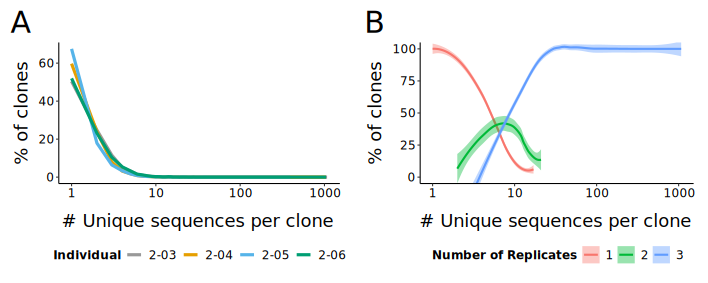
\includegraphics[width = 0.9\textwidth]{_Figures/png/pilot-clone-sizes}
\begin{subfigure}{0em}
\phantomsubcaption{}
\label{fig:igseq-pilot-clone-sizes-sizes}
\end{subfigure}
\begin{subfigure}{0em}
\phantomsubcaption{}
\label{fig:igseq-pilot-clone-sizes-reps}
\end{subfigure}
\caption{(A) Proportion of clones of different sizes for each individual in the pilot dataset, measured in unique sequences per clone. (B) Proportion of clones of each size found across one, two or all three replicates of the appropriate individual.}
% TODO: Add suitable overall figure title
\label{fig:igseq-pilot-clone-sizes}
\end{figure} % TODO: Correct subplot B legend spacing; describe smoothing plot better

\begin{figure}
\centering
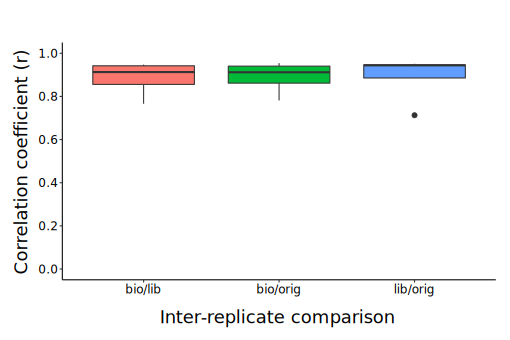
\includegraphics[width = 0.7\textwidth]{_Figures/png/pilot-clone-sizes-cor-boxplots}
\caption{Boxplots showing distribution of Pearson's product-moment correlation coefficients of clone sizes for each pair of replicates, as measured by the number of unique sequences per clone in each replicate. Clones absent in a given replicate were given a size of zero.}
% TODO: Add suitable overall figure title
\label{fig:igseq-pilot-clone-sizes-cor-boxplots}
\end{figure}

\begin{figure}
\centering
\includegraphics[width = 0.7\textwidth]{_Figures/png/pilot-clone-sizes-cor-scatter}
\caption{Scatter plots comparing clone sizes across biological replicates for each individual in the pilot dataset.}
% TODO: Add suitable overall figure title
\label{fig:igseq-pilot-clone-sizes-cor-scatter}
\end{figure}



% ********************************** Back Matter *******************************
% Backmatter should be commented out, if you are using appendices after References
%\backmatter

% ********************************** Bibliography ******************************
\begin{spacing}{0.9}

% To use the conventional natbib style referencing
% Bibliography style previews: http://nodonn.tipido.net/bibstyle.php
% Reference styles: http://sites.stat.psu.edu/~surajit/present/bib.htm

%\bibliographystyle{apalike}
%\bibliographystyle{unsrt} % Use for unsorted references 
% TODO: Fix bibliography style 
%\bibliographystyle{plainnat} % use this to have URLs listed in References
%\cleardoublepage
%\bibliography{D_References/igh-locus} % Path to your References.bib file
%\bibliography{D_References/Locus} % Path to your References.bib file

% If you would like to use BibLaTeX for your references, pass `custombib' as
% an option in the document class. The location of 'reference.bib' should be
% specified in the preamble.tex file in the custombib section.
% Comment out the lines related to natbib above and uncomment the following line.

\printbibliography[heading=bibintoc, title={References}]


\end{spacing}

% ********************************** Appendices ********************************

\begin{appendices} % Using appendices environment for more functionality
\appendix
%\addtocontents{toc}{\setcounter{tocdepth}{2}}
\chapter{Solutions and buffers}
\label{app:solutions}
\footnotesize
\section{Enzymes}
\label{app:solutions_enzymes}

\begin{threeparttable}
\begin{tabular}{lccc}\toprule
\textbf{Enzyme} & \textbf{Concentration} & \textbf{Manufacturer} & \textbf{Product code} \\\midrule
KAPA HiFi HotStart ReadyMix PCR Kit & \x{2}\tnote{a} & Kapa Biosystems & KR0370 \\
SMARTScribe Reverse Transcriptase & \unitsul{100} & Clontech Laboratories & 639537 \\
RNasin RNase inhibitor & \unitsul{40} & Promega &  N2511 \\
Uracil DNA glycosylase (UDG) & \unitsul{5} & NEB & M0280S \\
RNase A & \mgml{100} & QIAGEN & 19101 \\
\bottomrule \end{tabular}
\begin{tablenotes}
\item[a] KAPA HiFi HotStart DNA Polymerase present at \unitsul{0.04}.
\end{tablenotes}
\end{threeparttable}

\section{Non-enzyme reagents and components}
\label{app:solutions_reagents}

{\renewcommand{\arraystretch}{1.2}
\begin{threeparttable}
\begin{tabular}{lccc}\toprule
\textbf{Reagent} & \textbf{Concentration} & \textbf{Manufacturer} & \textbf{Product code} \\\midrule
SMARTScribe first-strand buffer & \x{5} & Clontech Laboratories & 639537\tnote{a}\\
Dithiothreitol (DTT) & \mmol{20} & Clontech Laboratories & 639537\tnote{a}\\
dNTP mix & \umol{10} each\tnote{b} & NEB & N0447L \\
\um{1} Sera-Mag Magnetic SpeedBeads & \mgml{50} & GE Healthcare & 65152105050250\\
QIAzol Lysis Reagent & \x{1} & QIAGEN & 79306\\
BluePippin electrophoresis buffer & \x{1} & Sage Science &BDF1510\tnote{c}\\
BluePippin R2 loading solution / marker mix & \x{1} & Sage Science &BDF1510\tnote{c}\\
Roti-Phenol/chloroform/isoamyl alcohol & \x{1} & Roth & A156.2\\
\bottomrule \end{tabular}
\begin{tablenotes}
\item[a] Supplied with SMARTScribe Reverse Transcriptase (\Cref{app:solutions_enzymes}).
\item[b] i.e. \umol{10} each of dATP, dGTP, dCTP and dTTP.
\item[c] Supplied with BluePippin \pc{1.5} agarose dye-free cassettes.
\end{tablenotes}
\end{threeparttable}
}

\section{Prepared buffers}
\label{app:solutions_buffers}
\begin{threeparttable}
\begin{tabular}{cllcc}\toprule
\textbf{Name} & \textbf{Purpose} & \textbf{Composition} & \textbf{pH} & \textbf{Storage temperature}\\\midrule
TET & Washing Sera-Mag beads & ~~\llap{\textbullet}~~ \mmol{10} Tris base & 8.0\tnote{a} & Room temperature \\
& & ~~\llap{\textbullet}~~ \mmol{1} Na\textsubscript{2}-EDTA & & \\
& & ~~\llap{\textbullet}~~ \pc{0.05} (v/v) Tween 20 & & \\\midrule
iSB & Preparing SeraSure bead suspension & ~~\llap{\textbullet}~~ \mol{4.2} NaCl & 8.0\tnote{a} & Room temperature \\
& & ~~\llap{\textbullet}~~ \mmol{16.8} Tris base & & \\
& & ~~\llap{\textbullet}~~ \mmol{1.68} Na\textsubscript{2}-EDTA & & \\\midrule
EB & Buffering nucleic-acid solutions & ~~\llap{\textbullet}~~ \mmol{10} Tris-HCl & 8.5\tnote{a} & Room temperature \\\midrule
P1 & Resuspending cultured \textit{E. coli} cells & ~~\llap{\textbullet}~~ \mmol{50} Tris-HCl}& 8\tnote{a} & \degC{4}\tnote{c} \\
& & ~~\llap{\textbullet}~~ \mmol{10} Na\textsubscript{2}-EDTA & & \\
& & ~~\llap{\textbullet}~~ \ugml{100} RNase-A\tnote{b} & & \\\midrule
P2 & Cell lysis & ~~\llap{\textbullet}~~ \mmol{200} Sodium hydroxide & -- & Room temperature \\
& & ~~\llap{\textbullet}~~ \pc{1} (v/v) Sodium dodecyl sulfate & & \\\midrule
P3 & Precipitation of cell lysate & ~~\llap{\textbullet}~~ \mol{3} Potassium acetate & 5.5\tnote{d} & Room temperature \\\midrule
\end{tabular}
\begin{tablenotes}
\item[a] Adjust to the required pH with hydrochloric acid (HCl).
\item[b] \Cref{app:solutions_enzymes}.
\item[c] Can be stored at room temperature before addition of RNase-A.
\item[d] Adjust to the required pH with glacial acetic acid.
\end{tablenotes}
\end{threeparttable}
%\afterpage{\begin{landscape}

\chapter{Primers and oligonucleotides}
\label{app:oligos}

\section{Template-switch adapter oligos for reverse transcription}
\label{app:oligos_tsa}

\begin{threeparttable}
\begin{tabular}{cp{11cm}cc}\toprule
\textbf{Name} & \textbf{Sequence} & \textbf{Source} \\\midrule
SmartNNNa & AAGCAGUGGTAUCAACGCAGAGUNNNNUNNNNUNNNNUCTTrGrGrGrG & \parencite{turchaninova2016igprep}\\
\bottomrule
\end{tabular}
\end{threeparttable}

\section{PCR and reverse-transcription primers}
\label{app:oligos_primers}

\begin{threeparttable}
\begin{tabular}{cp{7cm}cccc}\toprule
\textbf{Name} & \textbf{Sequence} & \textbf{Purpose} & \textbf{Source}\tnote{a} \\\midrule
\multirow{2}{*}{RT1} & \multirow{2}{*}{TGGTCTTGCCAGCTGGTGATTTCCGCC} & \igseq \cm{2} & \multirow{2}{*}{--} \\
 & & reverse-transcription primer & \\\midrule
M1SS & AAGCAGTGGTATCAACGCA & \igseq PCR1 forward primer & \parencite{turchaninova2016igprep} \\
IGH-B & CCACATGGCACCAGAGGAAAC & \igseq PCR1 reverse primer & --\\
M1S+P2 & GTGACTGGAGTTCAGACGTGTGCTCTTC--CGATCTCAGTGGTATCAACGCAGAG  & \igseq PCR2 forward primer & \parencite{turchaninova2016igprep} \\ % Plus Illumina adapters
IGH-C+P1 & ACACTCTTTCCCTACACGACGCTCTTC--CGATCTATGGCACCAGAGGAAACACAAC & \igseq PCR2 reverse primer & --\\
\bottomrule
\end{tabular}
\begin{tablenotes}
\item[a] Items without a specified source were designed by the author using \program{Primer3} \parencite{untergasser2012primer3}.
\end{tablenotes}
\end{threeparttable}

\newpage
\section{Illumina TruSeq adaptor sequences}
\label{app:oligos_illumina}

\subsection*{P1/i5 adaptor sequences}

\begin{tabular}{rm{10cm}}
\textbf{Base sequence:} & AATGATACGGCGACCACCGAGATCTACAC\textbf{NNNNNNNN}--ACACTCTTTCCCTACACGACGC\\
\textbf{Index sequences:} & \\
\end{tabular}\vspace{-2ex}

\begin{center}
\begin{threeparttable}
\begin{tabular}{cccc}\toprule
\textbf{Name} & \textbf{Index Sequence}\tnote{a}\\\midrule
D501 & AGGCTATA\\
D502 & GCCTCTAT\\
D503 & AGGATAGG\\
D504 & TCAGAGCC\\
D505 & CTTCGCCT\\
D506 & TAAGATTA\\
D507 & ACGTCCTG\\
D508 & GTCAGTAC\\
\bottomrule
\end{tabular}
\begin{tablenotes}
\item[a] \parencite{illumina2018adapters}
\end{tablenotes}
\end{threeparttable}
\end{center}

\subsection*{P2/i7 adaptor sequences}

\begin{tabular}{rm{10cm}}
\textbf{Base sequence:} & ACAAGCAGAAGACGGCATACGAGAT\textbf{NNNNNNNN}--GTGACTGGAGTTCAGACGTGTGC\\
\textbf{Index sequences:} & \\
\end{tabular}\vspace{-2ex}

\begin{center}
\begin{threeparttable}
\begin{tabular}{cccc}\toprule
\textbf{Name} & \textbf{Index Sequence}\tnote{a}\\\midrule
D701 & CGAGTAAT\\
D702 & TCTCCGGA\\
D703 & AATGAGCG\\
D704 & GGAATCTC\\
D705 & TTCTGAAT\\
D706 & ACGAATTC\\
D707 & AGCTTCAG\\
D708 & GCGCATTA\\
D709 & CATAGCCG\\
D710 & TTCGCGGA\\
D711 & GCGCGAGA\\
D712 & CTATCGCT\\
\bottomrule
\end{tabular}
\begin{tablenotes}
\item[a] \parencite{illumina2018adapters}
\end{tablenotes}
\end{threeparttable}
\end{center}

\chapter{Hill numbers and antibody repertoire diversity}
\label{app:diversity}

\normalsize

The question of how to measure the diversity of clones or sequences within an antibody repertoire, as well as the degree of divergence in composition between pairs or groups of repertoires, closely parallels related questions in ecology, information theory, and elsewhere. Over time, a great many different conceptions of diversity have been developed in these fields \citep{peet1974diversity}, each with its own cohort of measurement and approximation methods. Many of these diversity indices, however, can be unified into a common framework of so-called ``true diversities'' based on Hill numbers, providing a more intuitive and comprehensive insight into the diversity structure of a population. In this appendix, I describe the concepts and motivations underlying this conception of population of diversity, both for individual (unitary) populations (\Cref{app:diversity-unitary}) and for more complex populations with internal subpopulation structure (\Cref{app:diversity-structured}).

\section{Diversity in unitary populations}
\label{app:diversity-unitary}

\subsection{Terminology}
\label{app:diversity-unitary-terminology}

Though in this appendix I use terminology derived from the ecological literature, the concepts and measured discussed here can be applied to any situation in which a set (or \textit{population}) of elements (\textit{individuals}) is partitioned among some number of mutually-exclusive categories (\textit{species}). Considered abstractly, these terms and denotations could be used to refer to coloured balls in an urn, species in a rainforest, or sequences in a repertoire.

Let $X$ be a unitary population of individuals, each of which is assigned to some species $s$ from a set of possible species $S$. The term ``unitary'' here denotes that $X$ has no internal structure except the species identity of its constitutent individuals. Let $n_s$ denote the number of individuals in $X$ belonging to $s$, and $N$ denote the total number of individuals in $X$. Then 

\begin{equation}
p_s = \frac{n_s}{N}
\label{eq:species_proportion}
\end{equation}

\noindent denotes the proportion (or \textit{relative frequency}) of individuals in $X$ belonging to $s$, or equivalently the probability that a randomly-selected individual from $X$ belongs to $s$. The \textit{species richness} of $P$ is the total number of species $|S|$, while the \textit{evenness} of $P$ is the degree to which different species are similar in their $p_s$ values: a population containing one very abundant species and $n-1$ very rare species, for example, is much less even than a population containing $n$ equally-abundant species.

\subsection{Simple diversity indices}
\label{app:diversity-unitary-simple}

The diversity of a unitary population $X$ of some total size $N$ is generally considered to increase with both the richness and evenness of $X$. Different measures of within-population diversity, however, place different amounts of weight on the richness of $X$ compared to its evenness when evaluating its diversity. At one extreme, the species richness itself is used as a measure of diversity, albeit one that entirely ignores evenness; other commonly-used diversity measures, such as Simpson's index, Shannon entropy, and the Berger-Parker index are affected to varying degrees by both richness and evenness \parencite{peet1974diversity,berger1970diversity}. In addition to their relative emphasis on richness vs evenness, different indices will also place different amounts of weight on common vs rare species when computing diversity: at the extremes, species richness gives the same amount of weight to all species regardless of frequency, while the Berger-Parker index gives zero weight to all species except the most common (\Cref{app:diversity-unitary-simple-berger}). As a result, any given diversity index captures a different aspect of the diversity structure of any population of interest.

\subsubsection{Simpson's index}

One of the oldest diversity indices incorporating both species richness and evenness is Simpson's index, which measures the probability that two randomly selected individuals from a population are from the same species \citep{simpson1949diversity}. For a finite population (or sample) $X$ with a set of possible species $S$, Simpson's index is calculated as follows:

\begin{equation}
L(X) = \frac{\sum_{s \in S} n_s(n_s-1)}{N(N-1)}
\label{eq:simpson_finite}
\end{equation} 

\noindent As the population size tends to infinity, this value simplifies to

\begin{equation}
L^*(X) = \frac{\sum_{s \in S} n_s^2}{N^2} = \sum_{s \in S} p_s^2
\label{eq:simpson_finite}
\end{equation} 

\noindent As originally formulated, Simpson's index can be considered a \textit{dominance index} (also known as a concentration  index \citep{simpson1949diversity}), measuring the degree to which a population is dominated by a small number of species; as such, a higher Simpson's index indicates a less-diverse population. Conversely, the complement $1-L(P)$ of Simpson's index, known as the Gini-Simpson index \citep{jost2006entropy}, represents the ``probability of interspecific encounter'' \citep{peet1974diversity}, and is also widely used as a diversity index in the literature.

\subsubsection{The Berger-Parker index}
\label{app:diversity-unitary-simple-berger}

The Berger-Parker index is a very simple measure of diversity, given by the relative frequency $p_x$ of the most abundant species $x$ in the population \parencite{berger1970diversity,caruso2008bergerparker}. Like Simpson's index, the Berger-Parker is a dominance index, measuring the degree to which the population is dominated by the single largest species. Despite its simplicity, the Berger-Parker is a true diversity index, responding to both the richness and the evenness of a population, and can be used to distinguish different diversity structures in real populations \parencite{caruso2008bergerparker}. As it focuses only on the most common species in each population, it also has the particular advantage of being much less vulnerable to sampling bias than other diversity metrics, especially compared to the species richness itself \parencite{berger1970diversity}.

\subsubsection{Entropic diversity indices}
\label{app:diversity-unitary-simple-entropy}

In information theory, the Shannon entropy $H(Y)$ of a random variable $Y$ provides a measure of the unpredictability of that variable, and therefore of the degree to which its value can be predicted in advance \citep{shannon1948communication1}. A variable which can take only a single value has zero entropy (it is perfectly predictable), while one which can take all values in its state space with equal probability has maximum entropy (it is maximally unpredictable) for that state space. All else being equal, a variable which can take a larger number of possible values has greater entropy than one which can take fewer values; hence, the entropy of a variable increases with both the richness and evenness of its state space \citep{shannon1948communication1}.

Although the concept of Shannon entropy was developed in the context of electronic communication, it can be extended quite naturally to ecology, where the process of sampling species from a population represents an  information source and each species observation represents an output. In this case, the Shannon entropy represents  ``the amount of uncertainty that exists regarding the species of an individual selected at random from the population'' \citep{peet1974diversity}. The Shannon entropy of a population $X$ is given by

\begin{equation}
H(X) = -\sum_{s \in S} p_s \cdot \log p_s
\label{eq:shannon_infinite}
\end{equation}

\noindent Any base logarithm can be used, though bases $2$ and $e$ are most common; in these bases, the units of Shannon entropy are the bit (``binary digit'') and nat (``natural unit''), respectively.

A generalisation of the Shannon entropy, also used as a diversity measure, is the R\'{e}nyi entropy \parencite{mora2016renyi}:

\begin{equation}
H_q(X) = \frac{1}{1-q}\,\log\right[\sum_{s \in S} p_i^q\right]
\label{eq:renyi}
\end{equation}

\noindent where $q$ is denoted the \textit{order} of the entropy measure. The R\'{e}nyi entropy is undefined at $q = 1$, but reduces to the Shannon entropy (with the same base of logarithm) in the limit as $q \to 1$ \parencite{mora2016renyi}. As $p_i$ is always between 0 and 1, raising the relative frequencies to a power greater than 1 downweights rarer species (with smaller $p_i$) relative to more common ones; as a result, higher-order R\'{e}nyi entropies put more emphasis on the most common species compared to Shannon entropy when computing population diversity, while R\'{e}nyi entropies with order less than 1 put more weight on rarer species; at $q = 0$, $H_0$ is simply the logarithm of the species richness $|S|$.

\subsection{Effective species richness and true diversity}
\label{app:diversity-unitary-hill}

\Cref{app:diversity-unitary-simple} discusses several commonly-used diversity indices, including Simpson's index, the Gini-Simpson index, Shannon entropy (\& other R\'{e}nyi entropies), and the Berger-Parker index; many other diversity indices are possible. These indices differ importantly in their forms, numeric ranges and biological interpretation, as well as their response behaviours to different changes in population composition \citep{peet1974diversity, jost2006entropy}. For example, Simpson's index and the Berger-Parker index range from 0 to 1, with lower values indicating greater population diversity, while Shannon- and R\'{e}nyi-entropy measures range from 0 to infinity, with higher values indicating greater diversity (in log-scale). The use of different diversity indices can therefore yield importantly different results when used to compare different populations: comparing two populations using only one such measure will capture only part of the diversity structure of those populations, while comparing them using two or more raw indices will often yield results that are difficult to accurately interpret \citep{peet1974diversity, jost2006entropy}.

Fortunately, different diversity indices can be transformed into a common framework by considering, for each index, the number $D$ of \textit{equally-common} species that would be needed to produce the same diversity value using that index. This transformation gives an estimation, for each index, of the ``effective species richness'' of the population: if we corrected for differences in species abundance while holding the diversity index constant, how rich would the resulting population be? This effective richness can itself be considered a diversity measure; one that is comparable across diversity indices in a way the raw indices are not \citep{jost2006entropy}.

For many important diversity indices, the equation for the effective richness $D$ takes a common form, known as the Hill number or ``true diversity'' for some parameter $q$ \citep{hill1973diversity, jost2006entropy}:

\begin{equation}
^qD(X) = \left(\sum_{s \in S} p_s^q \right)^{\frac{1}{1-q}}
\label{eq:hill_index}
\end{equation}

\noindent Indices whose effective richnesses take this form (\Cref{tab:diversity}) include species richness ($q=0$), R\'{e}nyi entropy in base $e$ ($q=q$), Shannon entropy in base $e$ ($q \to 1$), Simpson's index ($q = 2$) and the Berger-Parker index ($q \to \infty$) among others \citep{peet1974diversity, hill1973diversity, jost2006entropy, miho2018strategies}. As with the R\'{e}nyi entropy, the parameter $q$, known here as the \textit{diversity order}, describes the degree to which rare species are downweighted compared to common ones when calculating the Hill number: at one extreme ($q=0$, the species richness), all species are given equal weight regardless of their frequency, while at the other ($q \to \infty$, the reciprocal Berger-Parker index) only the most common species in the sample is considered. As a result of this downweighting, higher-order indices are also less sensitive to undersampling than lower-order ones; this is particularly important to keep in mind in cases, like immune repertoires, where the number of rare species is extremely large and undersampling of rare species is pervasive \parencite{mora2016diversity}.

The use of Hill numbers in diversity estimation enables many different, widely-used diversity measurements to be considered and compared in a common framework, giving a description of population diversity that is easy to interpret biologically and compare across different populations \parencite{jost2006entropy}. Typically, the limit at $q \to 1$ is substituted for the (undefined) value at $q = 1$, giving a function that is both continuous and monotonically decreasing:

\begin{equation}
^qD(X) = \begin{cases} \left(\displaystyle\sum_{s \in S} p_s^q \right)^{\frac{1}{1-q}} & q \neq 1\\
\exp\left(-\displaystyle\sum_{s \in S}p_s \cdot \ln p_s\right) & q = 1 \end{cases}
\label{eq:hill_index_continuous}
\end{equation}

\noindent This equation can then be easily used to construct diversity profiles (or \textit{spectra}) spanning many different orders of diversity \citep{miho2018strategies}; since each value of $q$ captures a different aspect of a population's diversity structure, these profiles can be much more informative than any single metric when analysing and comparing the diversity structure of populations.

\begin{table}
\centering
\caption{Summary of effective richness measures for some common diversity indices (adapted and expanded from \citep{jost2006entropy})}
\begin{tabular}{lll}\toprule
Diversity index, $f(X)$ & Effective species richness,~$^qD(X)$ & Diversity order, $q$\\\midrule
Species richness & $^0D(X) = f(X)$ & 0 \\
Shannon entropy (base $e$) & $\lim_{q \to 1}~^qD(X) = \exp\,f(X)$ & 1\\
Simpson index & $^2D(X) = \frac{1}{f(X)}$ & 2\\
Gini-Simpson index & $^2D(X) = \frac{1}{1-f(X)}$ & 2\\
Renyi entropy (base $e$, order $q$) & $^qD(X) = \exp\,f(X)$ & $q$\\
Berger-Parker index & $\lim_{q \to \infty}~^qD(X) = \frac{1}{f(X)}$ & $\infty$\\
\bottomrule
\end{tabular}
\label{tab:diversity}
\end{table}

\section{Diversity in structured populations}
\label{app:diversity-structured}

Section \ref{app:diversity-unitary} discusses methods for analysing the diversity of a single, unitary population. In many cases, however, we are interested in groups of related populations, and the relative amount of variability within and between the populations in each group. In order to extend the mathematical framework of diversity measurement, and especially that of true diversities and Hill spectra, to this more complex case, some additional clarification of terminology is needed.

\subsection{Terminology}
\label{app:diversity-structured-terminology}

In a \textit{structured} population $C$, the individuals in $C$ can be partitioned into some number $M$ of disjoint unitary subpopulations $X_1, X_2, \dots$, such that:

\begin{itemize} % Itemize or enumerate?
\item Each subpopulation $X$ has size $N_X$, with the total size of the whole population given by $N = \sum_{X \in C}~N_X$.
\item Each individual in a subpopulation $X$ is assigned to a species $s$ drawn from a set of possible species $S_X$, with the total species set for the population given by $S = \bigcup_{X \in C}~S_X$.
\item Each subpopulation can be assigned a relative statistical weight $w_X$; this could be equal for all populations ($w_X = 1/M$), proportional to each population's relative size $w_X = \frac{N_X}{N}$, or proportional to some other measure of each population's ``importance'' to the system.
\item The relative frequency of a species $s$ in a subpopulation $X$ is given by $p_{X,\,s} = \frac{n_{X,\,s}}{N_X}$, where $n_{X,\,s}$ is the number of individuals in $X$ belonging to $s$.
\end{itemize}

\noindent What is the diversity of $C$? There are several possible answers, depending on which features of the makeup of $C$ are most salient:

\begin{enumerate}
\item The \textbf{gamma diversity} of $C$ is the \textit{total} diversity of the population when its subpopulations are pooled according to their weights; it represents the species diversity across the whole population, ignoring the subpopulation membership of individuals.
\item The \textbf{alpha diversity} of $C$ is the diversity arising from differences in species identity among individuals \textit{within} each subpopulation, and is given by a weighted \textit{average} of the unitary diversities of those subpopulations; the appropriate weighting function depends on the order of diversity under consideration. In some sense, the alpha diversity of $C$ can be thought of as the expected diversity of a single population drawn from $C$.
\item The \textbf{beta diversity} of $C$ is the diversity arising from variability in species composition \textit{among} the subpopulations in $C$; it is lowest when all subpopulations have identical species compositions and highest when they have no species in common.
\end{enumerate}

\noindent The alpha and beta diversities of a population are independent; two different structured populations can have identical alpha and very different beta diversities, or vice versa, depending on the exact species compositions of their subpopulations. The alpha and beta diversity of a structured population also completely determine its gamma diversity \citep{jost2007partitioning}:

\begin{equation}
D_\gamma(C) = D_\alpha(C) \times D_\beta(C)
\label{eq:diversity_relationship_gamma}
\end{equation}

\noindent and therefore 

\begin{equation}
D_\beta = \frac{D_\gamma}{D_\alpha}
\label{eq:diversity_relationship_beta}
\end{equation}

\noindent This (\autoref{eq:diversity_relationship_beta}) is typically the easiest way of computing the beta diversity of a given collection of populations.

In the rest of this section, I will primarily consider only subpopulations with equal sizes $N_X = \frac{N}{M}$ and equal weights $w = \frac{1}{M}$, as this is how they are used in the repertoire-diversity methods discussed in \Cref{sec:methods_comp_igdownstream_spectra} and \Cref{chap:igseq}. Equal-sized and -weighted populations can be produced by downsampling each subpopulation to the same number of individuals (in the \igseq case, by downsampling each repertoire to the same number of unique sequences) prior to calculating the diversity of the population.
 
\subsubsection{Calculating alpha, beta, and gamma}
\label{app:diversity-structured-calc}

The alpha, beta and gamma diversities of structured populations can be calculated analogously to the unitary true diversities discussed in \Cref{app:diversity-unitary-hill}. In this framework, the alpha diversity represents the effective number of equally-abundant species present in the ``average'' subpopulation drawn from $C$, while the gamma diversity represents the effective number of such species present in the population as a whole (ignoring subpopulation membership). Beta diversity also represents an effective number of groupings, but in this case the unit is subpopulations rather than species: given an alpha diversity value for $C$, the beta diversity gives the number of equally-weighted subpopulations, with no species in common, that would give rise to the gamma diversity of $C$.

Under this framework, the diversities of order $q$ for a structured population $C$ are given by

% TODO: Cite or explain these equations

\begin{equation}
^qD_\gamma(C)
= \left[\sum_{s \in S} \left(\frac{\displaystyle\sum_{X \in C} w_Xp_{X,\,s}}{\displaystyle\sum_{X \in C} w_X}\right)^q\right]^\frac{1}{1-q}
= \left[\frac{\displaystyle\sum_{s \in S}\left(\sum_{X \in C} w_Xp_{X,\,s}\right)^q}{\displaystyle\left(\sum_{X \in C} w_X\right)^q}\right]^\frac{1}{1-q}
\label{eq:diversity_gamma}
\end{equation}

\begin{equation}
^qD_\alpha(C)
= \left[\frac{\displaystyle\sum_{X \in C} w_X^q \left(\sum_{s \in S_X} p_{X,\,s}^q\right)}{\displaystyle\sum_{X \in C} w_X^q}\right]^\frac{1}{1-q}
= \left[\frac{\displaystyle\sum_{X \in C}\sum_{s \in S_X} (w_Xp_{X,\,s})^q}{\displaystyle\sum_{X \in C} w_X^q}\right]^\frac{1}{1-q}
\label{eq:diversity_alpha}
\end{equation}

\begin{equation}
^qD_\beta(C) = \frac{^qD_\gamma(C)}{^qD_\alpha(C)}
= \left[
\frac{\displaystyle\sum_{s \in S}\left(\sum_{X \in C} w_Xp_{X,\,s}\right)^q}
{\displaystyle\sum_{X \in C}\sum_{s \in S_X} (w_Xp_{X,\,s})^q}
\times
\frac{\displaystyle\sum_{X \in C} w_X^q}
{\displaystyle\left(\sum_{X \in C} w_X\right)^q}
\right]^\frac{1}{1-q}
\label{eq:diversity_beta}
\end{equation}

\noindent When all the subpopulations are equally-weighted (i.e. $w_X = w = \frac{1}{M}$ for all subpopulations), these formulae simplify considerably:

\begin{equation}
^qD_\gamma(C)
= \left[\frac{\displaystyle\sum_{s \in S}\left(\sum_{X \in C} wp_{X,\,s}\right)^q}{\displaystyle\left(\sum_{X \in C} w\right)^q}\right]^\frac{1}{1-q}
= \left[\frac{\displaystyle w^q\sum_{s \in S}\left(\sum_{X \in C} p_{P,s}\right)^q}{\displaystyle M^qw^q}\right]^\frac{1}{1-q}
= \left[\frac{\displaystyle\sum_{s \in S}\left(\sum_{X \in C} p_{X,\,s}\right)^q}{\displaystyle M^q}\right]^\frac{1}{1-q}
\label{eq:diversity_gamma_even}
\end{equation}

\begin{equation}
^qD_\alpha(C)
= \left[\frac{\displaystyle\sum_{X \in C}\sum_{s \in S_X} (wp_{X,\,s})^q}{\displaystyle\sum_{X \in C} w^q}\right]^\frac{1}{1-q}
= \left[\frac{\displaystyle w^q\sum_{X \in C}\sum_{s \in S_X} (p_{X,\,s})^q}{\displaystyle M w^q}\right]^\frac{1}{1-q}
= \left[\frac{\displaystyle \sum_{X \in C}\sum_{s \in S_X} (p_{X,\,s})^q}{\displaystyle M}\right]^\frac{1}{1-q}
\label{eq:diversity_alpha_even}
\end{equation}

\begin{equation}
^qD_\beta(C) = \frac{^qD_\gamma(C)}{^qD_\alpha(C)}
= \left[
\frac{\displaystyle\sum_{s \in S}\left(\sum_{X \in C} p_{X,\,s}\right)^q}{\displaystyle \sum_{X \in C}\sum_{s \in S_X} (p_{X,\,s})^q}
\times
\frac{\displaystyle M}{\displaystyle M^q}
\right]^\frac{1}{1-q}
= \left[
\frac{\displaystyle\sum_{s \in S}\left(\sum_{X \in C} p_{X,\,s}\right)^q}{\displaystyle M^{q-1} \sum_{X \in C}\sum_{s \in S_X} (p_{X,\,s})^q}
\right]^\frac{1}{1-q}
\label{eq:diversity_beta_even}
\end{equation}

\noindent These equations are valid for all values of $q \in \mathbb{R}$ except 1, providing a spectrum of alpha, beta or gamma diversity measures analogous to the diversity spectra provided for unitary populations in \Cref{app:diversity-unitary-hill}. As in the unitary case, a special case needs to be made for $q = 1$ in order to make these functions continuous\footnote{Note that, when $w = \frac{1}{M}$ and $N_X = \frac{N}{M}$ for all populations, $\displaystyle\sum_{X \in C}wp_{X,\,s} = \sum_{X \in C}\frac{1}{M}\frac{n_{X,\,s}}{N_X} = \frac{1}{M}\frac{M \sum_{X \in C} n_{X,\,s}}{N} = \frac{n_{s}}{N} = p_s$} \parencite{jost2007partitioning}:

\begin{equation}
\begin{split}
^1D_\gamma(C) & = \lim_{q \to 1} {^qD}_\gamma(C)
= \exp\left[-\sum_{s \in S}\left(\left[\sum_{X \in C}wp_{X,\,s}\right]\cdot\ln \left[\sum_{X \in C}wp_{X,\,s}\right]\right)\right]\\
& = \exp\left(-\sum_{s \in S}p_s \cdot\ln p_s\right) =\:^1D(C)
\end{split}
\label{eq:diversity_gamma_q1}
\end{equation}

\begin{equation}
\begin{split}
^1D_\alpha(C) & = \lim_{q \to 1} {^qD}_\alpha(C)
= \exp\left[-\sum_{X \in C}w\sum_{s \in S_X}(p_{X,\,s}\cdot\ln p_{X,\,s})\right]\\
 & = \exp\left[\frac{1}{M}\sum_{X \in C}\left(-\sum_{s \in S_X}(p_{X,\,s}\cdot\ln p_{X,\,s})\right)\right] = \exp\left[\frac{1}{M}\sum_{X \in C}\ln\,^1D(X)\right]
\end{split}
\label{eq:diversity_alpha_q1}
\end{equation}

\begin{equation}
\begin{split}
^1D_\beta(C) & = \frac{^1D_\gamma(C)}{^1D_\alpha(C)} = \frac{\exp\left[-\sum_{s \in S}p_s \cdot\ln p_s\right]}{\exp\left[\frac{1}{M}\sum_{X \in C}\left(-\sum_{s \in S_X}(p_{X,\,s}\cdot\ln p_{X,\,s})\right)\right]} = \frac{\exp\left[\frac{1}{M}\sum_{X \in C}\ln\,^1D(X)\right]}{^1D(C)}
\end{split}
\label{eq:diversity_beta_q1}
\end{equation}

\subsubsection{Rescaling beta diversity}
\label{app:diversity-structured-rescaling}

As discussed in \Cref{app:diversity-structured-calc}, while alpha  and gamma diversity are expressed in terms of an effective number of species (in an average subpopulation and the entire structured population, respectively), beta diversity is expressed in terms of an effective number of subpopulations. Since the effective number of subpopulations is determined in part by the actual number of subpopulations, this means that the beta diversity, unlike alpha and gamma diversity, is directly dependent on the number of subpopulations $M$. If two different structured populations contain different numbers of subpopulations, it is therefore not possible to compare their beta diversity values directly; rather, the beta diversity spectra of the populations must be \textit{rescaled} to a common range before such a comparison is performed.

The \textit{minimum} beta diversity of a structured population obtains when all subpopulations have identical species competition (i.e. $p_{X,\,s} = p_{s}$ for all species $s$ and subpopulations $X$). In this case, the beta diversity for the structured population is given by:

\begin{equation}
^qD_{\beta\min}(C) = \left[
\frac{\displaystyle\sum_{s \in S}\left(\sum_{X \in C} p_{X,\,s}\right)^q}{\displaystyle M^{q-1} \sum_{X \in C}\sum_{s \in S_X} (p_{X,\,s})^q}
\right]^\frac{1}{1-q}
= \left[
\frac{\displaystyle\sum_{s \in S}\left(Mp_s\right)^q}{\displaystyle M^{q-1}\sum_{s \in S_X} Mp_s^q}
\right]^\frac{1}{1-q}
= \left[
\frac{M^q\displaystyle\sum_{s \in S}p_s^q}{M^q\displaystyle\sum_{s \in S_X} p_s^q}
\right]^\frac{1}{1-q} = 1
\label{eq:diversity_beta_min}
\end{equation}

\noindent The \textit{maximum} beta diversity, meanwhile, obtains when there is no overlap in species between populations. In this case, for any given species, $n_{X,\,s}$ is equal to $n_s$ for one subpopulation and $0$ for all others, and therefore $\left(\sum_{X \in C} p_{X,\,s}\right)^q = \sum_{X \in C} (p_{X,\,s})^q = p_s^q$~~and~~$\sum_{X \in C}\sum_{s \in S_X} (p_{X,\,s})^q = \sum_{s \in S} p_s^q$. The beta diversity is therefore given by:

\begin{equation}\begin{split}
^qD_{\beta\max}(C) &
= \left[\frac{\displaystyle\sum_{s \in S}\left(\sum_{X \in C} p_{X,\,s}\right)^q}{\displaystyle M^{q-1} \sum_{X \in C}\sum_{s \in S_X} (p_{X,\,s})^q}\right]^\frac{1}{1-q}
= \left[\frac{\displaystyle\sum_{s \in S} p_s^q}{\displaystyle M^{q-1} \sum_{s \in S} p_s^q}\right]^\frac{1}{1-q}
= \left[\frac{1}{M^{q-1}}\right]^\frac{1}{1-q} = \boldsymbol{M}
\end{split}
\label{eq:diversity_beta_max}
\end{equation}

\noindent The same identities hold for the special case when $q = 1$:

\begin{equation}
\begin{split}
^1D_{\beta\min}(C) & = \frac{\exp\left[-\sum_{s \in S}p_s \cdot\ln p_s\right]}{\exp\left[\frac{1}{M}\sum_{X \in C}\left(-\sum_{s \in S_X}(p_{X,\,s}\cdot\ln p_{X,\,s})\right)\right]} = \frac{\exp\left[-\sum_{s \in S}p_s \cdot\ln p_s\right]}{\exp\left[\frac{1}{M}\sum_{X \in C}\left(-\sum_{s \in S}(p_{s}\cdot\ln p_{s})\right)\right]}\\
& = \frac{\exp\left[-\sum_{s \in S}p_s \cdot\ln p_s\right]}{\exp\left[\frac{M}{M}\left(-\sum_{s \in S}p_{s}\cdot\ln p_{s}\right)\right]} = \boldsymbol{1}
\end{split}
\label{eq:diversity_beta_q1_min}
\end{equation}

\begin{equation}\begin{split}
^1D_{\beta\max}(C)
& = \frac{\exp\left[-\sum_{s \in S}p_s \cdot\ln p_s\right]}{\exp\left[\frac{1}{M}\sum_{X \in C}\left(-\sum_{s \in S_X}(p_{X,\,s}\cdot\ln p_{X,\,s})\right)\right]}\\
& = \exp\left[-\sum_{s \in S}p_s \cdot\ln p_s - \frac{1}{M}\sum_{X \in C}\left(-\sum_{s \in S_X}(p_{X,\,s}\cdot\ln p_{X,\,s})\right)\right]\\
& = \exp\left[H(C) + \frac{1}{M}\sum_{X \in C}\left(\sum_{s \in S_X}\frac{n_{X,\,s}}{N_X}\cdot\ln \frac{n_{X,\,s}}{N_X}\right)\right]\\
& = \exp\left[H(C) + \frac{1}{M}\sum_{X \in C}\left(\sum_{s \in S_X}\frac{Mn_{X,\,s}}{N}\cdot\ln \frac{Mn_{X,\,s}}{N}\right)\right]\\
& = \exp\left[H(C) + \sum_{X \in C}\left(\sum_{s \in S_X}\frac{n_{X,\,s}}{N}\cdot\ln \frac{Mn_{X,\,s}}{N}\right)\right]\\
& = \exp\left[H(C) + \left(\sum_{s \in S}\frac{n_{s}}{N}\cdot\ln \frac{Mn_{s}}{N}\right)\right]
 = \exp\left[H(C) + \left(\sum_{s \in S}p_s\cdot\ln (Mp_s)\right)\right]\\
& = \exp\left[H(C) + \left(\sum_{s \in S}p_s\cdot\left[\ln M + \ln p_s\right]\right)\right]\\
& = \exp\left[H(C) + \left(\sum_{s \in S}p_s\cdot\ln p_s\right)+ \ln M \cdot \sum_{s \in S}p_s\right]
= \exp\left[H(C) - H(C) + \ln M\right]\\
& = \exp\ln M = \boldsymbol{M}
\end{split}
\label{eq:diversity_beta_q1_max}
\end{equation}

\noindent The beta diversity for a structured population with $M$ subpopulations therefore ranges between $1$ (identical composition) and $M$ (maximally-divergent composition). The beta diversities of this population can thus be transformed onto a new scale from $0$ to $1$ as follows:

\begin{equation}
^qD_{\beta\,\mathrm{rescaled}} = \frac{^qD_\beta -\:^qD_{\beta\min}}{^qD_{\beta\max} -\: ^qD_{\beta\min}} = \frac{^qD_\beta - 1}{M - 1}
\label{eq:diversity_beta_rescale}
\end{equation}

\noindent By transforming the beta diversity spectra of different structured populations onto this common scale, the inter-subpopulation variability of those populations can be meaningfully compared, even if they differ in the number of subpopulations they contain.
\chapter{Supplementary figures}
\label{app:figures}

% 3 - LOCUS CHAPTER

\begin{figure}
	\centering
	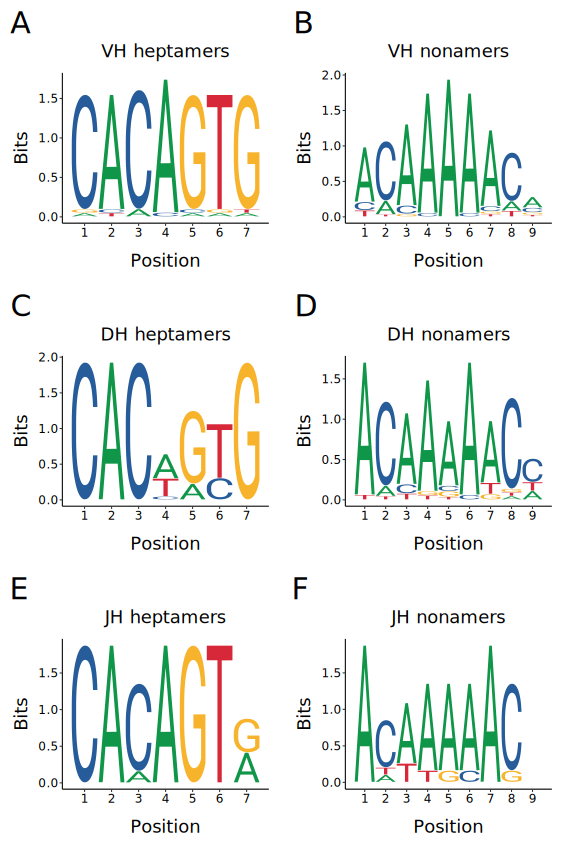
\includegraphics[width=0.9\textwidth]{_Figures/png/nfu-rss-seqlogo-sep}
	\caption[\Nfu recombination signal sequences by segment type]{\textbf{\Nfu recombination signal sequences by segment type:} Sequence composition of conserved heptamer (A,C,E) and nonamer (B,D,F) sequences from \Nfu heavy-chain RSSs associated with \vh (A,B), \dh (C,D) or \jh (E,F) gene segments.}
	\label{fig:nfu-rss-seqlogo-sep}
\end{figure}

\begin{figure}
	\centering
	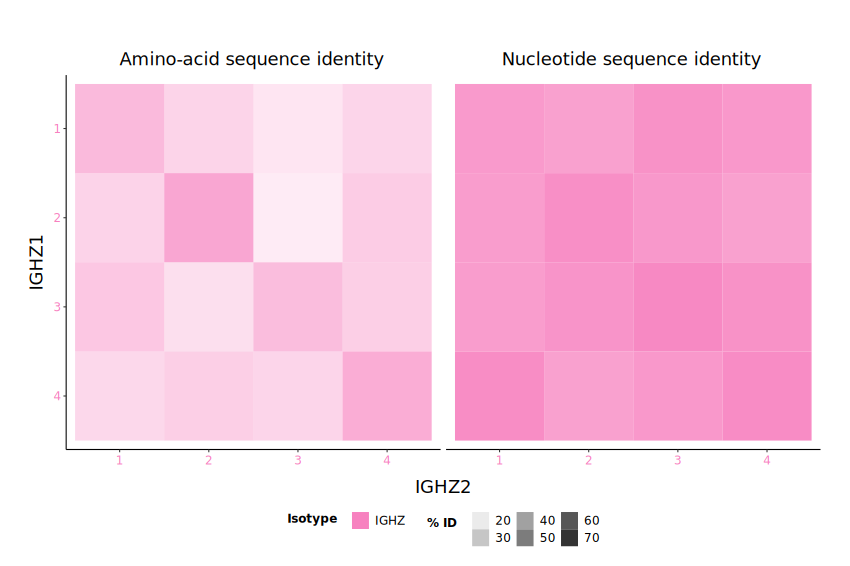
\includegraphics[width=0.8\textwidth]{_Figures/png/xma-new-cz-aln}
	\caption[Sequence similarity between \igh{Z} constant-regions in \Xma]{\textbf{Sequence similarity between \igh{Z} constant-regions in \Xma:} Heatmap of percentage sequence identity between amino-acid (right) and nucleotide (left) sequences of \cz{} exons from the two \Xma \igh{Z} constant regions, calculated using pairwise Needleman-Wunsch global alignments.} % TODO: Combine isotype and identity legends
	\label{fig:xma-cz-aln}
\end{figure}

	\begin{figure}
	\centering
	\includegraphics[width=\textwidth]{_Figures/png/xma-vh-families-map}
	\caption[Heatmap of \vh families in the in \Xma \textit{IgH} locus]{\textbf{Heatmap of \vh families in the in \Xma (\textit{IgH}) locus:} Heatmap of family relationships among \Xma \vh segments, with coloured shading indicating families and red dots indicating pairwise nucleotide sequence identity of at least 80\%. \vh families containing multiple segments are uniquely coloured, while single-segment families are in grey.}
	\label{fig:xma-vh-families-map}
	\end{figure}

	\begin{figure}
	\centering
	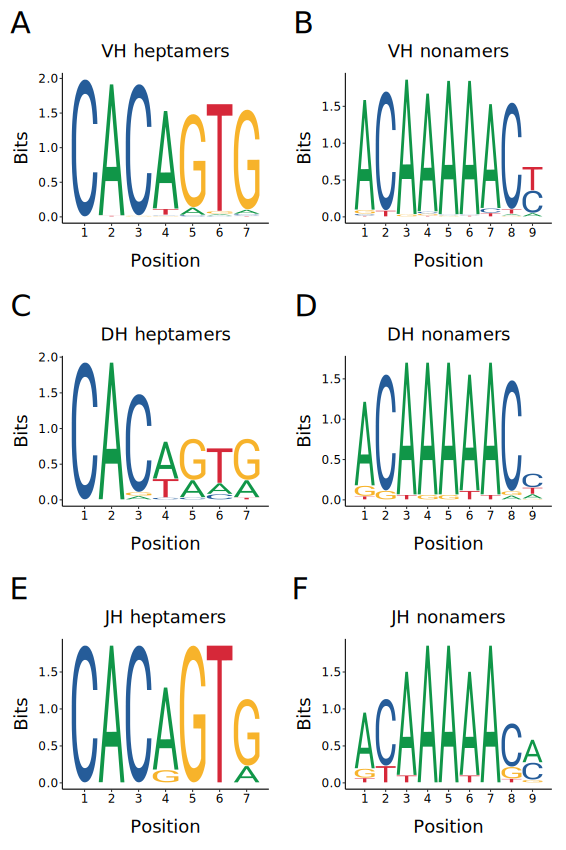
\includegraphics[width=0.9\textwidth]{_Figures/png/xma-new-rss-seqlogo-sep}
	\caption[\Xma recombination signal sequences by segment type]{\textbf{\Xma recombination signal sequences by segment type:} Sequence composition of conserved heptamer (A,C,E) and nonamer (B,D,F) sequences from \Xma heavy-chain RSSs associated with \vh (A,B), \dh (C,D) or \jh (E,F) gene segments.}
	\label{fig:xma-rss-seqlogo-sep}
	\end{figure}
\chapter{Supplementary tables}
\label{app:tables}

\begin{table}
\caption{Software versions used in computational analyses}
\label{tab:software-versions}
\centering
% latex table generated in R 3.5.2 by xtable 1.8-3 package
% Sun Mar 17 19:16:12 2019
\begin{tabular}{ll}
  \toprule Program & Version \\ 
  \midrule Basemount & 0.15.96.2154 \\ 
  BLAST & 2.7.1 \\ 
  Bowtie 2 & 2.2.6 \\ 
  CD-HIT-EST & 4.6.8 \\ 
  Change-O & 0.4.5 \\ 
  EMBOSS (FUZZNUC) & 6.6.0 \\ 
  FigTree & 1.4.2 \\ 
  HMMER & 3.2 \\ 
  IgBLAST & 1.7.0 \\ 
  IGoR & 1.3.0 \\ 
  IGV & 2.3.68 \\ 
  IMGT/DomainGapAlign & 4.9.2 \\ 
  PRANK & v.170427 \\ 
  pRESTO & 0.5.10 \\ 
  Primer3 & 2.3.6 \\ 
  Python 2 & 2.7.14 \\ 
  Python 3 & 3.6.4 \\ 
  QuorUM & 1.0.0 \\ 
  R & 3.4.1/3.5.2 \\ 
  RAxML & 8.2.12 \\ 
  RepeatMasker & 4.0.6 \\ 
  SAMtools & 1.9 \\ 
  sed & 4.2.2 \\ 
  seqtk & 1.3 \\ 
  Snakemake & 5.3.0 \\ 
  SPAdes & 3.6.1 \\ 
  SSPACE & 3.0 \\ 
  STAR & 2.5.2b \\ 
  Trimmomatic & 0.32 \\ 
  VSEARCH & 2.8.0 \\ 
   \bottomrule \end{tabular}

\end{table}

\begin{table}
\caption{RNA-sequencing datasets used for \textit{IGH} locus characterisation}
\centering
\begin{threeparttable}
\begin{tabular}{>{\bfseries}c|c|c}\toprule
Species & \Nfu & \Xma \\\midrule
Tissues & Gut & Various\tnote{a}\\\midrule
BioProject Accession & PRJNA379208 & PRJNA420092\\\midrule
\multirow{26}{*}{SRA Run Accessions} & SRR5344350 & SRR6327069\\
& SRR5344343 & SRR6327070\\
& SRR5344344 & SRR6327071\\
& SRR5344345 & SRR6327072\\
& SRR5344346 & SRR6327073\\
& SRR5344347 & SRR6327074\\
& SRR5344348 & SRR6327075\\
& SRR5344349 & SRR6327076\\
& SRR5344350 & SRR6327077\\
&&SRR6327078\\
&&SRR6327079\\
&&SRR6327080\\
&&SRR6327081\\
&&SRR6327082\\
&&SRR6327083\\
&&SRR6327084\\
&&SRR6327085\\
&&SRR6327086\\
&&SRR6327087\\
&&SRR6327088\\
&&SRR6327089\\
&&SRR6327090\\
&&SRR6327091\\
&&SRR6327092\\
&&SRR6327093\\
&&SRR6327094\\\midrule
Source & \parencite{smith2017microbiota} & Citation not given\\
\bottomrule\end{tabular}
	\begin{tablenotes}
	\item[a] Tissues used for \Xma RNA-sequencing included brain, heart, liver, gut, skin or whole fish; see BioProject entry for details.
	\end{tablenotes}
\end{threeparttable}
\label{tab:rnaseq-sources}
\end{table}

% 3 - LOCUS CHAPTER
\centering

\begin{table}\centering
    \caption{Co-ordinate table of constant-region exons in the \Nfu \igh{} locus}
    	% latex table generated in R 3.5.2 by xtable 1.8-3 package
% Tue Jan 15 17:07:52 2019
\begin{tabular}{llrrrl}
  \toprule Name & Isotype & Start & End & Length & Strand \\ 
  \midrule IGH1M-1 & M & 130848 & 131144 & 297 & + \\ 
  IGH1M-2 & M & 131971 & 132312 & 342 & + \\ 
  IGH1M-3 & M & 132394 & 132705 & 312 & + \\ 
  IGH1M-4 & M & 132816 & 133288 & 473 & + \\ 
  IGH1M-TM1 & M & 134262 & 134413 & 152 & + \\ 
  IGH1M-TM2 & M & 138431 & 138819 & 389 & + \\ 
  IGH1D-1 & D & 139381 & 139689 & 309 & + \\ 
  IGH1D-2A & D & 139774 & 140064 & 291 & + \\ 
  IGH1D-3A & D & 140178 & 140489 & 312 & + \\ 
  IGH1D-4A & D & 140572 & 140853 & 282 & + \\ 
  IGH1D-2B & D & 145613 & 145909 & 297 & + \\ 
  IGH1D-3B & D & 146000 & 146311 & 312 & + \\ 
  IGH1D-4B & D & 146398 & 146676 & 279 & + \\ 
  IGH1D-5 & D & 146795 & 147124 & 330 & + \\ 
  IGH1D-6 & D & 147210 & 147527 & 318 & + \\ 
  IGH1D-7 & D & 147598 & 147885 & 288 & + \\ 
  IGH1D-TM1 & D & 148016 & 148164 & 149 & + \\ 
  IGH1D-TM2 & D & 148323 & 148504 & 182 & + \\ 
  IGH2D-TM2 & D & 187624 & 187803 & 180 & - \\ 
  IGH2D-TM1 & D & 187963 & 188111 & 149 & - \\ 
  IGH2D-7 & D & 188658 & 188945 & 288 & - \\ 
  IGH2D-6 & D & 189016 & 189333 & 318 & - \\ 
  IGH2D-5 & D & 189419 & 189748 & 330 & - \\ 
  IGH2D-4B & D & 189867 & 190145 & 279 & - \\ 
  IGH2D-3B & D & 190232 & 190543 & 312 & - \\ 
  IGH2D-2B & D & 190636 & 190932 & 297 & - \\ 
  IGH2D-4A & D & 195644 & 195925 & 282 & - \\ 
  IGH2D-3A & D & 196008 & 196319 & 312 & - \\ 
  IGH2D-2A & D & 196433 & 196723 & 291 & - \\ 
  IGH2D-1 & D & 196808 & 197116 & 309 & - \\ 
  IGH2M-TM2 & M & 198315 & 198506 & 192 & - \\ 
  IGH2M-TM1 & M & 199834 & 199985 & 152 & - \\ 
  IGH2M-4 & M & 200953 & 201425 & 473 & - \\ 
  IGH2M-3 & M & 201536 & 201847 & 312 & - \\ 
  IGH2M-2 & M & 201929 & 202270 & 342 & - \\ 
  IGH2M-1 & M & 203549 & 203845 & 297 & - \\ 
   \bottomrule \end{tabular}

    \label{tab:nfu-ch-coords}
\end{table}

    \begin{landscape}
        \centering
        \vspace*{\fill}
        \scriptsize
		% latex table generated in R 3.5.2 by xtable 1.8-3 package
% Fri Jan  4 11:18:28 2019
\begin{tabular}{lrrrlrlrlrrl}
  \toprule Name & Start & End & Length & Strand & RSS Start & Heptamer & Spacer Length & Nonamer & RSS End & RSS Length & Comment \\ 
  \midrule IGH1V1-01 & 1252 & 1540 & 289 & + & 1541 & CACAGTG & 22 & ACAAAAACC & 1578 & 38 &  \\ 
  IGH1V1-02 & 3365 & 3656 & 292 & + & 3657 & CACAGTG & 22 & ACAAAAACC & 3694 & 38 &  \\ 
  IGH1V2-01 & 5907 & 6201 & 295 & + & 6202 & CACAGAA & 15 & ACAAAAACT & 6232 & 31 &  \\ 
  IGH1V1-03 & 13690 & 13964 & 275 & + & 13965 & CACAGTG & 22 & ACAAAAACC & 14002 & 38 &  \\ 
  IGH1V3-01 & 14862 & 15162 & 301 & + & 15163 & CACAGTG & 23 & ACAAAAACC & 15201 & 39 &  \\ 
  IGH1V2-02 & 17433 & 17730 & 298 & + & 17731 & CACAATG & 23 & ACAAAAACC & 17769 & 39 &  \\ 
  IGH1V4-01 & 24566 & 24837 & 272 & + & 24838 & CGCAGTG & 22 & CCACAAACC & 24875 & 38 & Nonsense mutation \\ 
  IGH1V1-04 & 37305 & 37596 & 292 & + & 37597 & CACAGTG & 22 & ACAAAAACC & 37634 & 38 &  \\ 
  IGH1V2-03 & 48845 & 49139 & 295 & + & 49140 & CACAGTG & 23 & TCAAAAACT & 49178 & 39 &  \\ 
  IGH1V1-05 & 49909 & 50197 & 289 & + & 50198 & CACAGTG & 22 & ACAAAAACC & 50235 & 38 &  \\ 
  IGH1V5-01 & 51710 & 51998 & 289 & + & 51999 & CACAGTG & 22 & ACAAAAACT & 52036 & 38 &  \\ 
  IGH1V2-04 & 56322 & 56616 & 295 & + & 56617 & CACAGTG & 23 & ACAAAAACC & 56655 & 39 &  \\ 
  IGH1V6-01 & 57465 & 57762 & 298 & + & 57763 & CACAGTG & 21 & ACTAAATCT & 57799 & 37 &  \\ 
  IGH1V1-06 & 59678 & 59966 & 289 & + & 59967 & CACAGTG & 22 & ACAAAAACC & 60004 & 38 &  \\ 
  IGH1V4-02 & 68017 & 68288 & 272 & + & 68289 & TGCAGTG & 22 & TCACAAACC & 68326 & 38 & Nonsense mutation \\ 
  IGH1V2-05 & 69787 & 70084 & 298 & + & 70085 & CACAGTG & 23 & ACAAAAACC & 70123 & 39 &  \\ 
  IGH1V1-07 & 155485 & 155763 & 279 & + & 155764 & CACAGTG & 22 & TCAAAACCC & 155801 & 38 &  \\ 
  IGH2V2-02 & 282620 & 282914 & 295 & - & 282915 & CACAGTG & 23 & ACAAAAACC & 282953 & 39 &  \\ 
  IGH2V4-01 & 284404 & 284675 & 272 & - & 284676 & TGCAGTG & 22 & TCACAAACC & 284713 & 38 & Nonsense mutation \\ 
  IGH2V5-01 & 288808 & 289096 & 289 & - & 289097 & CACAGTG & 22 & ACAGAAACT & 289134 & 38 &  \\ 
  IGH2V1-03 & 289977 & 290271 & 295 & - & 290272 & CACAGTG & 22 & ACAAAAACC & 290309 & 38 &  \\ 
  IGH2V1-02 & 293835 & 294126 & 292 & - & 294127 & CACAGTG & 22 & ACAAAAACC & 294164 & 38 &  \\ 
  IGH2V2-01 & 303780 & 304074 & 295 & - & 304075 & CAGGGCC & 24 & AGCACAAAG & 304114 & 40 &  \\ 
  IGH2V1-01 & 304926 & 305204 & 279 & - & 305205 & CACAGTG & 22 & TCAAAACCC & 305242 & 38 &  \\ 
   \bottomrule \end{tabular}

		\normalsize\vspace{1em}
        \captionof{table}{Co-ordinate table of \vh segments in the \Nfu \igh{} locus}
        \label{tab:nfu-vh-coords}
        \vspace*{\fill}
    \end{landscape}

        {\centering
        \captionof{table}{Co-ordinate table of \dh segments in the \Nfu \igh{} locus}\vspace{-0.3em}
        \label{tab:nfu-dh-coords-seg}
        \scriptsize
		% latex table generated in R 3.5.2 by xtable 1.8-3 package
% Tue Jan 15 17:07:52 2019
\begin{tabular}{lrlrrl}
  \toprule Name & Start & NT Sequence & End & Length & Strand \\ 
  \midrule IGH1D01 & 25782 & ATACGTACTTTCGTGGTATATAGAGA & 25807 & 26 & + \\ 
  IGH1D02 & 76700 & GATATCTGGGTGGGGG & 76715 & 16 & + \\ 
  IGH1D03 & 77027 & TGAAATGATTAC & 77038 & 12 & + \\ 
  IGH1D04 & 77476 & TCGCGTAGCGGC & 77487 & 12 & + \\ 
  IGH1D05 & 78717 & GAAACCACGGCAGC & 78730 & 14 & + \\ 
  IGH1D06 & 79049 & TTTATAGCGGCTAC & 79062 & 14 & + \\ 
  IGH1D07 & 80417 & CAGACTGGAGA & 80427 & 11 & + \\ 
  IGH1D08 & 81362 & TTCATGGCAGCCAC & 81375 & 14 & + \\ 
  IGH1D09 & 82067 & CAGACTGGAGC & 82077 & 11 & + \\ 
  IGH1D10 & 84282 & TGGGGTGGCAGC & 84293 & 12 & + \\ 
  IGH2D04 & 263497 & CAGACTGGAGA & 263507 & 11 & - \\ 
  IGH2D03 & 270243 & TTTATAGCGGCTAC & 270256 & 14 & - \\ 
  IGH2D02 & 270878 & GAAACCACGGCAGC & 270891 & 14 & - \\ 
  IGH2D01 & 271749 & GACTTTTACTAC & 271760 & 12 & - \\ 
   \bottomrule \end{tabular}

		\normalsize\vspace{1em}
        \captionof{table}{Co-ordinate table of \dh 5'-RSSs in the \Nfu \igh{} locus}\vspace{-0.3em}
        \label{tab:nfu-dh-coords-rss5}
        \scriptsize
        	% latex table generated in R 3.5.2 by xtable 1.8-3 package
% Fri Jan  4 11:18:28 2019
\begin{tabular}{lrlrlrr}
  \toprule Name & 5'-RSS Start & Nonamer & Spacer Length & Heptamer & 5'-RSS End & Length \\ 
  \midrule IGH1D01 & 25754 & GGTTGTTGT & 12 & CACTGTG & 25781 & 28 \\ 
  IGH1D02 & 76672 & AGTTTTTGA & 12 & CACAGTG & 76699 & 28 \\ 
  IGH1D03 & 76999 & TGTTGTTGT & 12 & CACAGTG & 77026 & 28 \\ 
  IGH1D04 & 77448 & AGTTTTTGT & 12 & CACGGTG & 77475 & 28 \\ 
  IGH1D05 & 78688 & GATGTTTTT & 13 & CACAGTG & 78716 & 29 \\ 
  IGH1D06 & 79021 & TGTTTTTGT & 12 & CGCTGTG & 79048 & 28 \\ 
  IGH1D07 & 80417 & AGTTTTGGT & 12 & CACAGTG & 80444 & 28 \\ 
  IGH1D08 & 81334 & TGTTTTTGT & 12 & CGCTGTG & 81361 & 28 \\ 
  IGH1D09 & 82039 & AGTTTTGGT & 12 & CACAGTG & 82066 & 28 \\ 
  IGH1D10 & 84254 & TCATTCATT & 12 & CACTGTG & 84281 & 28 \\ 
  IGH2D04 & 263497 & AGTTTTGGT & 12 & CACAGTG & 263524 & 28 \\ 
  IGH2D03 & 270215 & TGTTTTTGT & 12 & CGCTGTG & 270242 & 28 \\ 
  IGH2D02 & 270850 & TGTTTTTGT & 12 & CACAGTG & 270877 & 28 \\ 
  IGH2D01 & 271721 & AGTTTTTAT & 12 & CATGGTG & 271748 & 28 \\ 
   \bottomrule \end{tabular}

        	\normalsize\vspace{1em}
        \captionof{table}{Co-ordinate table of \dh 3'-RSSs in the \Nfu \igh{} locus}\vspace{-0.3em}
        \label{tab:nfu-dh-coords-rss3}
        \scriptsize
		% latex table generated in R 3.5.2 by xtable 1.8-3 package
% Tue Jan 15 17:07:52 2019
\begin{tabular}{lrlrlrr}
  \toprule Name & 3'-RSS Start & Heptamer & Spacer Length & Nonamer & 3'-RSS End & Length \\ 
  \midrule IGH1D01 & 25808 & CACAGTG & 12 & ACAAAAACC & 25835 & 28 \\ 
  IGH1D02 & 76716 & CACAGTG & 12 & ACAAAAACC & 76743 & 28 \\ 
  IGH1D03 & 77039 & CACTGTG & 11 & AATATAACC & 77065 & 27 \\ 
  IGH1D04 & 77488 & CACAGCG & 12 & ACATAAAAC & 77515 & 28 \\ 
  IGH1D05 & 78731 & CACAGCG & 12 & ACAAAAGCC & 78758 & 28 \\ 
  IGH1D06 & 79063 & CACTGTG & 12 & ACAAGATCC & 79090 & 28 \\ 
  IGH1D07 & 80428 & CACAACG & 12 & ACAAAAACC & 80455 & 28 \\ 
  IGH1D08 & 81376 & CACTGTG & 12 & ACAAAATCC & 81403 & 28 \\ 
  IGH1D09 & 82078 & CACAATG & 12 & ACAAAAACC & 82105 & 28 \\ 
  IGH1D10 & 84294 & CACAGTG & 12 & ACAAAAACC & 84321 & 28 \\ 
  IGH2D04 & 263508 & CACAACG & 12 & ACAAAAACC & 263535 & 28 \\ 
  IGH2D03 & 270257 & CACTGTG & 12 & ACAAGATCC & 270284 & 28 \\ 
  IGH2D02 & 270892 & CACAGCG & 12 & ACAAAAGCC & 270919 & 28 \\ 
  IGH2D01 & 271761 & CACAATG & 12 & ACAAAAACC & 271788 & 28 \\ 
   \bottomrule \end{tabular}

		\normalsize
		}

    \begin{landscape}
        \centering
        \notsotiny
		% latex table generated in R 3.5.2 by xtable 1.8-3 package
% Tue Jan 15 17:07:52 2019
\begin{tabular}{lrllrrl}
  \toprule Name & Start & NT Sequence & AA Sequence & End & Length & Strand \\ 
  \midrule IGH1J01 & 26187 & GTGCTTTAGACAACTGGGGAAAAGGAACGGAGGTTACTGTTCAACCTG & ALDNWGKGTEVTVQP & 26234 & 48 & + \\ 
  IGH1J02 & 128176 & ATGACTACTTTGACTACTGGGGAAAAGGAACAATGGTGACGGTCACATCAG & DYFDYWGKGTMVTVTS & 128226 & 51 & + \\ 
  IGH1J03 & 128354 & ACCGTGGGGTAAAGGGACAACAGTCACGGTCAAAACAG & PWGKGTTVTVKT & 128391 & 38 & + \\ 
  IGH1J04 & 128533 & ACGGTGCTCTTGACTACTGGGGTAAAGGGACCGCAGTCACTGTAACATCAG & GALDYWGKGTAVTVTS & 128583 & 51 & + \\ 
  IGH1J05 & 128887 & ACAACGCTTTTGACTACTGGGGAAAAGGAACAACGGTCACCGTCACTTCAG & NAFDYWGKGTTVTVTS & 128937 & 51 & + \\ 
  IGH1J06 & 129346 & CTACGATGCTTTTGACTACTGGGGGAAAAGGACGATGGTCACGTCACTTCAG & YDAFDYWGKRTMVTSLQ & 129397 & 52 & + \\ 
  IGH1J07 & 129635 & TTAACTGGGCTTTCGACTACTGGGGAAAAGGGACGATGGTAACGGTGACTTCAG & NWAFDYWGKGTMVTVTS & 129688 & 54 & + \\ 
  IGH1J08 & 129965 & TTACCACGCAGCTTTGGACTACTGGGGAAAAGGGACGACGGTCACCGTCACCTCAG & YHXALDYWGKGTTVTVTS & 130020 & 56 & + \\ 
  IGH1J09 & 130612 & TCTACGCTGCTTTTGACTACTGGGGTAAAGGTACAACGGTAACCGTTTCATCAG & YAAFDYWGKGTTVTVSS & 130665 & 54 & + \\ 
  IGH2J08 & 204031 & TCTACGCTGCTTTTGACTACTGGGGTAAAGGTACAACGGTAACCGTTTCATCAG & YAAFDYWGKGTTVTVSS & 204084 & 54 & - \\ 
  IGH2J07 & 204673 & TTACCACGCAGCTTTGGACTACTGGGGAAAAGGGACGACGGTCACCGTCACCTCAG & YHXALDYWGKGTTVTVTS & 204728 & 56 & - \\ 
  IGH2J06 & 205005 & ATAACTGGGCTTTCGACTACTGGGGAAAAGGGACGATGGTAACGGTGACTTCAG & NWAFDYWGKGTMVTVTS & 205058 & 54 & - \\ 
  IGH2J05 & 205296 & CTACGATGCTTTTGACTACTGGGGGAAAAGGACGATGGTCACGTCACTTCAG & YDAFDYWGKRTMVTSLQ & 205347 & 52 & - \\ 
  IGH2J04 & 205756 & ACAACGCTTTTGACTACTGGGGAAAAGGAACAACGGTCACCGTCACTTCAG & NAFDYWGKGTTVTVTS & 205806 & 51 & - \\ 
  IGH2J03 & 206111 & ATGGTGCTTTTGACTACTGGGGTAAAGGGACCGCAGTCACTGTAACATCAG & GAFDYWGKGTAVTVTS & 206161 & 51 & - \\ 
  IGH2J02 & 206303 & ACCGTGGGGTAAAGGGACAACAGTCACGGTCAAAACAG & PWGKGTTVTVKT & 206340 & 38 & - \\ 
  IGH2J01 & 206466 & ATGACTACTTTGACTACTGGGGAAAAGGAACAATGGTGACGGTCACATCAG & DYFDYWGKGTMVTVTS & 206516 & 51 & - \\ 
   \bottomrule \end{tabular}

		\normalsize\vspace{0.6em}
        \captionof{table}{Co-ordinate table of \jh segments in the \Nfu \igh{} locus}
        \label{tab:nfu-jh-coords-seg}
        \notsotiny
		% latex table generated in R 3.5.2 by xtable 1.8-3 package
% Tue Jan 15 17:07:52 2019
\begin{tabular}{lrlrlrr}
  \toprule Name & RSS Start & Nonamer & Spacer Length & Heptamer & RSS End & RSS Length \\ 
  \midrule IGH1J01 & 26196 & TGTTTTTGT & 23 & CACTGTG & 26186 & 39 \\ 
  IGH1J02 & 128188 & AGTGTTTGT & 23 & CACTGTG & 128175 & 39 \\ 
  IGH1J03 & 128353 & TGTTTATTT & 23 & CACTGTG & 128353 & 39 \\ 
  IGH1J04 & 128545 & GGTTTTTGT & 23 & CACTGTG & 128532 & 39 \\ 
  IGH1J05 & 128899 & GGTTTTAGT & 23 & TACTGTG & 128886 & 39 \\ 
  IGH1J06 & 129360 & TCTTCTTGT & 22 & TACTTTG & 129345 & 38 \\ 
  IGH1J07 & 129650 & AGTTTTTGT & 23 & TACTGTG & 129634 & 39 \\ 
  IGH1J08 & 129983 & AGTTTTAGT & 22 & TACTGTG & 129964 & 38 \\ 
  IGH1J09 & 130628 & CGTTTTTAT & 22 & CACTGTG & 130611 & 38 \\ 
  IGH2J08 & 204047 & CGTTTTTAT & 22 & CACTGTG & 204030 & 38 \\ 
  IGH2J07 & 204691 & AGTTTTAGT & 22 & TACTGTG & 204672 & 38 \\ 
  IGH2J06 & 205020 & AGTTTTTGT & 23 & TACTGTG & 205004 & 39 \\ 
  IGH2J05 & 205310 & TCTTCTTGT & 22 & TACTTTG & 205295 & 38 \\ 
  IGH2J04 & 205768 & GGTTTTAGT & 23 & TACTGTG & 205755 & 39 \\ 
  IGH2J03 & 206123 & GGTTTTTGT & 23 & CACTGTG & 206110 & 39 \\ 
  IGH2J02 & 206302 & TGTTTATTT & 23 & CACTGTG & 206302 & 39 \\ 
  IGH2J01 & 206478 & AGTGTTTGT & 23 & CACTGTG & 206465 & 39 \\ 
   \bottomrule \end{tabular}

		\normalsize\vspace{0.6em}
        \captionof{table}{Co-ordinate table of \jh RSSs in the \Nfu \igh{} locus}
        \label{tab:nfu-jh-coords-rss}
    \end{landscape}

\begin{table}\centering
    \caption{Co-ordinate table of constant-region exons in the \Xma \igh{} locus}
    	% latex table generated in R 3.5.2 by xtable 1.8-3 package
% Tue Jan  8 15:33:35 2019
\begin{tabular}{llrrrl}
  \toprule Name & Isotype & Start & End & Length & Strand \\ 
  \midrule IGHZ1-1 & Z & 3380 & 3667 & 288 & + \\ 
  IGHZ1-2 & Z & 3814 & 4098 & 285 & + \\ 
  IGHZ1-3 & Z & 4195 & 4497 & 303 & + \\ 
  IGHZ1-4 & Z & 4934 & 5263 & 330 & + \\ 
  IGHZ1-S & Z & 5264 & 5459 & 196 & + \\ 
  IGHZ1-TM1 & Z & 6345 & 6490 & 146 & + \\ 
  IGHZ1-TM2 & Z & 6645 & 7043 & 399 & + \\ 
  IGHZ2-1 & Z & 256059 & 256337 & 279 & + \\ 
  IGHZ2-2 & Z & 256453 & 256734 & 282 & + \\ 
  IGHZ2-3 & Z & 256893 & 257171 & 279 & + \\ 
  IGHZ2-4 & Z & 257319 & 257636 & 318 & + \\ 
  IGHZ2-S & Z & 257637 & 257850 & 214 & + \\ 
  IGHZ2-TM1 & Z & 258059 & 258213 & 155 & + \\ 
  IGHZ2-TM2 & Z & 258410 & 258629 & 220 & + \\ 
  IGHM-1 & M & 279664 & 279960 & 297 & + \\ 
  IGHM-2 & M & 280880 & 281224 & 345 & + \\ 
  IGHM-3 & M & 281321 & 281629 & 309 & + \\ 
  IGHM-4 & M & 281789 & 282291 & 503 & + \\ 
  IGHM-TM1 & M & 282910 & 283034 & 125 & + \\ 
  IGHM-TM2 & M & 285028 & 285740 & 713 & + \\ 
  IGHD-1 & D & 285902 & 286219 & 318 & + \\ 
  IGHD-2A & D & 286310 & 286597 & 288 & + \\ 
  IGHD-3A & D & 286814 & 287128 & 315 & + \\ 
  IGHD-4A & D & 287250 & 287534 & 285 & + \\ 
  IGHD-2B & D & 288876 & 289166 & 291 & + \\ 
  IGHD-3B & D & 289262 & 289576 & 315 & + \\ 
  IGHD-4B & D & 289680 & 289964 & 285 & + \\ 
  IGHD-5 & D & 290052 & 290381 & 330 & + \\ 
  IGHD-6 & D & 290472 & 290789 & 318 & + \\ 
  IGHD-7 & D & 290865 & 291152 & 288 & + \\ 
  IGHD-TM1 & D & 291286 & 291434 & 149 & + \\ 
  IGHD-TM2 & D & 291541 & 291642 & 102 & + \\ 
   \bottomrule \end{tabular}

    \label{tab:xma-ch-coords}
\end{table}

    \begin{landscape}
        \centering
        \vspace*{\fill}
        \scriptsize
		% latex table generated in R 3.5.2 by xtable 1.8-3 package
% Tue Jan  8 15:33:33 2019
\begin{tabular}{lrrrlrlllrrl}
  \toprule Name & Start & End & Length & Strand & RSS Start & Heptamer & Spacer Length & Nonamer & RSS End & RSS Length & Comment \\ 
  \midrule IGHV01-01 & 1159 & 1450 & 292 & + & 1451 & CACAGTG & 23 & GTAAAAACC & 1489 & 39 &  \\ 
  IGHV02-01 & 10534 & 10825 & 292 & + & 10826 & CACAGTG & 23 & ACAAAACCC & 10864 & 39 &  \\ 
  IGHV02-02 & 11961 & 12261 & 301 & + & 12262 & CACTGTG & 23 & ACAAAAACT & 12300 & 39 &  \\ 
  IGHV02-03 & 13319 & 13616 & 298 & + & 13617 & CACAGTG & 23 & ACACAAACT & 13655 & 39 &  \\ 
  IGHV03-01 & 15440 & 15734 & 295 & + & 15735 & CACAGTG & 22 & ACAAAAACT & 15772 & 38 &  \\ 
  IGHV02-04 & 16618 & 16908 & 291 & + & 16909 & CACAGTG & 23 & ACAAAAACC & 16947 & 39 &  \\ 
  IGHV02-05 & 17522 & 17822 & 301 & + & 17823 & CACTGTG & 22 & ACAAAAACT & 17860 & 38 &  \\ 
  IGHV02-06 & 18881 & 19178 & 298 & + & 19179 & CACAGTG & 23 & ACACAAACT & 19217 & 39 &  \\ 
  IGHV03-02 & 21000 & 21294 & 295 & + & 21295 & CACAGTG & 22 & ACAAAAACT & 21332 & 38 &  \\ 
  IGHV02-07 & 22179 & 22467 & 289 & + & 22468 & CACAGTG & 23 & ACAAAAACC & 22506 & 39 &  \\ 
  IGHV02-08p & 24234 & 24514 & 281 & + & 24515 & CACAGTG & 23 & ACAAAAACT & 24553 & 39 & Frameshift \\ 
  IGHV04-01 & 25359 & 25659 & 301 & + & 25660 & CACAGTG & 23 & ACAAAAACT & 25698 & 39 &  \\ 
  IGHV04-02 & 27066 & 27366 & 301 & + & 27367 & CACAGTG & 23 & ACAAAAACA & 27405 & 39 &  \\ 
  IGHV02-09 & 28669 & 28958 & 290 & + & 28959 & CACAGTG & 23 & ACAAAAACC & 28997 & 39 &  \\ 
  IGHV02-10p & 30460 & 30741 & 282 & + & 30742 & CACAATG & 23 & ACAAAACTC & 30780 & 39 & Frameshift \\ 
  IGHV02-11 & 32395 & 32681 & 287 & + & 32682 & CACAGTG & 23 & ACAAAAACC & 32720 & 39 &  \\ 
  IGHV03-03 & 33663 & 33957 & 295 & + & 33958 & CACTGTG & 22 & ACAAAAACT & 33995 & 38 &  \\ 
  IGHV02-12 & 35012 & 35299 & 288 & + & 35300 & CACAGTG & 23 & ACAAAAACC & 35338 & 39 &  \\ 
  IGHV03-04 & 36281 & 36575 & 295 & + & 36576 & CACTGTG & 22 & ACAAAAACT & 36613 & 38 &  \\ 
  IGHV02-13 & 37639 & 37931 & 293 & + & 37932 & CACAGTG & 23 & ACAAAAACT & 37970 & 39 &  \\ 
  IGHV02-14 & 39019 & 39311 & 293 & + & 39312 & CACAGTG & 23 & ACAAAAACT & 39350 & 39 &  \\ 
  IGHV03-05 & 41008 & 41302 & 295 & + & 41303 & CACAGTG & 22 & ACAAAAACT & 41340 & 38 &  \\ 
  IGHV02-15 & 42660 & 42952 & 293 & + & 42953 & CACAGTG & 23 & ACAAAAACT & 42991 & 39 &  \\ 
  IGHV03-06 & 45081 & 45375 & 295 & + & 45376 & CACAGTG & 22 & ACAAAAACT & 45413 & 38 &  \\ 
  IGHV02-16 & 46732 & 47024 & 293 & + & 47025 & CACAGTG & 23 & ACAAAAACT & 47063 & 39 &  \\ 
   \bottomrule \end{tabular}

		\normalsize\vspace{1em}
        \captionof{table}{Co-ordinate table of \vh segments in the \Xma \igh{} locus, part 1}
        \label{tab:xma-vh-coords-1}
        \vspace*{\fill}
    \end{landscape}

    \begin{landscape}
        \centering
        \vspace*{\fill}
        \scriptsize
		% latex table generated in R 3.5.2 by xtable 1.8-3 package
% Tue Jan  8 15:33:33 2019
\begin{tabular}{lrrrlrlllrrl}
  \toprule Name & Start & End & Length & Strand & RSS Start & Heptamer & Spacer Length & Nonamer & RSS End & RSS Length & Comment \\ 
  \midrule IGHV03-07 & 48618 & 48912 & 295 & + & 48913 & CACAGTG & 22 & ACAAAAACT & 48950 & 38 &  \\ 
  IGHV02-17 & 50323 & 50611 & 289 & + & 50612 & CACAGTG & 23 & ACAAAAACC & 50650 & 39 &  \\ 
  IGHV03-08 & 51890 & 52184 & 295 & + & 52185 & CACAGTG & 22 & ACAAAAACT & 52222 & 38 &  \\ 
  IGHV03-09p & 53026 & 53274 & 249 & + & 53275 &  &  &  &  &  & 3'-truncated, no RSS \\ 
  IGHV02-18 & 54462 & 54747 & 286 & + & 54748 & CACAGTG & 23 & ACAAAAACC & 54786 & 39 &  \\ 
  IGHV02-19p & 55729 & 55866 & 138 & + & 55867 & CACAGTG & 23 & ACAAAAACC & 55905 & 39 & 3'-truncated \\ 
  IGHV03-10 & 57371 & 57662 & 292 & + & 57663 & CACAGTG & 22 & ACAAAAACT & 57700 & 38 &  \\ 
  IGHV02-20p & 58698 & 58986 & 289 & + & 58987 & CACAGTG & 23 & ATAAAAACC & 59025 & 39 & Nonsense mutation \\ 
  IGHV03-11 & 59940 & 60234 & 295 & + & 60235 & CACAGTG & 22 & ACAAAAACT & 60272 & 38 &  \\ 
  IGHV02-21 & 61249 & 61537 & 289 & + & 61538 & CACAGTG & 23 & ATAAAAACC & 61576 & 39 &  \\ 
  IGHV03-12 & 62491 & 62785 & 295 & + & 62786 & CACAGTG & 22 & ACAAAAACT & 62823 & 38 &  \\ 
  IGHV02-22 & 63801 & 64089 & 289 & + & 64090 & CACAGTG & 23 & ATAAAAACC & 64128 & 39 &  \\ 
  IGHV03-13 & 65043 & 65337 & 295 & + & 65338 & CACAGTG & 22 & ACAAAAACT & 65375 & 38 &  \\ 
  IGHV02-23 & 66354 & 66640 & 287 & + & 66641 & CACAGTG & 23 & ACAAAAACT & 66679 & 39 &  \\ 
  IGHV03-14 & 68452 & 68743 & 292 & + & 68744 & CACTATG & 22 & ACAAAACTC & 68781 & 38 &  \\ 
  IGHV02-24 & 70101 & 70389 & 289 & + & 70390 & CACAGTG & 23 & ACAAAAACC & 70428 & 39 &  \\ 
  IGHV03-15 & 72206 & 72501 & 296 & + & 72502 & CACAGTG & 22 & ACAAAAACT & 72539 & 38 &  \\ 
  IGHV02-25 & 73484 & 73772 & 289 & + & 73773 & CACAGTG & 23 & ACAAAAACC & 73811 & 39 &  \\ 
  IGHV03-16 & 75799 & 76090 & 292 & + & 76091 & CACAGTG & 22 & ACAAAAACT & 76128 & 38 &  \\ 
  IGHV03-17 & 77773 & 78067 & 295 & + & 78068 & CACAGTG & 22 & ACAAAAACT & 78105 & 38 &  \\ 
  IGHV02-26 & 79001 & 79289 & 289 & + & 79290 & CACAGTG & 23 & ACAAAAACC & 79328 & 39 &  \\ 
  IGHV03-18 & 80492 & 80784 & 293 & + & 80785 & CACAGTG & 22 & ACAAAAACT & 80822 & 38 &  \\ 
  IGHV02-27p & 81799 & 82082 & 284 & + & 82083 & CACAGTG & 23 & ACAAAAACC & 82121 & 39 & Frameshift \\ 
  IGHV03-19 & 83736 & 84030 & 295 & + & 84031 & CACAGTG & 22 & ACAAAAACT & 84068 & 38 &  \\ 
  IGHV02-28p & 85093 & 85381 & 289 & + & 85382 & CACAGGG & 23 & GCAAAAACC & 85420 & 39 & Nonsense mutation \\ 
   \bottomrule \end{tabular}

		\normalsize\vspace{1em}
        \captionof{table}{Co-ordinate table of \vh segments in the \Xma \igh{} locus, part 2}
        \label{tab:xma-vh-coords-2}
        \vspace*{\fill}
    \end{landscape}

    \begin{landscape}
        \centering
        \vspace*{\fill}
        \scriptsize
		% latex table generated in R 3.5.2 by xtable 1.8-3 package
% Tue Jan  8 15:33:33 2019
\begin{tabular}{lrrrlrlllrrl}
  \toprule Name & Start & End & Length & Strand & RSS Start & Heptamer & Spacer Length & Nonamer & RSS End & RSS Length & Comment \\ 
  \midrule IGHV02-29 & 86225 & 86505 & 281 & + & 86506 & CACAGTG & 23 & ATAAAAACC & 86544 & 39 &  \\ 
  IGHV03-20 & 87419 & 87713 & 295 & + & 87714 & CACAGTG & 22 & ACAAAAACT & 87751 & 38 &  \\ 
  IGHV03-21 & 94532 & 94826 & 295 & + & 94827 & CACAGTG & 23 & ACAAAAACC & 94865 & 39 &  \\ 
  IGHV03-22 & 96192 & 96489 & 298 & + & 96490 & CACAGTG & 23 & ACAAAAACC & 96528 & 39 &  \\ 
  IGHV03-23 & 98068 & 98368 & 301 & + & 98369 & CACAGTG & 23 & ACAAAAACC & 98407 & 39 &  \\ 
  IGHV03-24 & 99482 & 99779 & 298 & + & 99780 & CACAGTG & 23 & ACAAAAACC & 99818 & 39 &  \\ 
  IGHV03-25 & 101639 & 101936 & 298 & + & 101937 & CACAGTG & 23 & ACAAAAACC & 101975 & 39 &  \\ 
  IGHV05-01p & 102818 & 103096 & 279 & + & 103097 & CAGAAGC & 0 & ACAAAAACT & 103112 & 16 & Frameshift \\ 
  IGHV03-26 & 104098 & 104389 & 292 & + & 104390 & CACAGTG & 23 & ACAAAATCC & 104428 & 39 &  \\ 
  IGHV06-01 & 105551 & 105831 & 281 & + & 105832 & CACAGTG & 23 & ACAAAAACC & 105870 & 39 &  \\ 
  IGHV03-27 & 107274 & 107571 & 298 & + & 107572 & CACAGTG & 23 & ACAAAAACC & 107610 & 39 &  \\ 
  IGHV03-28 & 108775 & 109072 & 298 & + & 109073 & CACAGAG & 23 & ACAAAAACC & 109111 & 39 &  \\ 
  IGHV03-29 & 110372 & 110672 & 301 & + & 110673 & CACAGTG & 23 & ACAAAAACC & 110711 & 39 &  \\ 
  IGHV07-01 & 111565 & 111856 & 292 & + & 111857 & CACAATG & 23 & ACAAAAACT & 111895 & 39 &  \\ 
  IGHV08-01p & 113033 & 113330 & 298 & + & 113331 & CACAGAG & 23 & CCAAGAACC & 113369 & 39 & Nonsense mutation \\ 
  IGHV09-01 & 115512 & 115800 & 289 & + & 115801 & CACAGTG & 22 & ACAAAAACT & 115838 & 38 &  \\ 
  IGHV10-01 & 117078 & 117379 & 302 & + & 117380 & CACAGTG & 22 & ACATAAACT & 117417 & 38 &  \\ 
  IGHV11-01 & 119462 & 119760 & 299 & + & 119761 & CACAGTG & 23 & ACAAAAACT & 119799 & 39 &  \\ 
  IGHV03-30 & 126125 & 126416 & 292 & + & 126417 & CACAGTG & 22 & ACAAAAACC & 126454 & 38 &  \\ 
  IGHV03-31 & 127109 & 127400 & 292 & + & 127401 & CACAGTG & 23 & GCAAAAACC & 127439 & 39 &  \\ 
  IGHV12-01 & 128489 & 128786 & 298 & + & 128787 & CACAGTG & 23 & ACAAAAACC & 128825 & 39 &  \\ 
  IGHV02-30 & 135711 & 136000 & 290 & + & 136001 & CACAGTG & 22 & ACAAAAACA & 136038 & 38 &  \\ 
  IGHV13-01 & 136757 & 137057 & 301 & + & 137058 & CACAGTG & 23 & ACAAAAACT & 137096 & 39 &  \\ 
  IGHV02-31 & 138344 & 138637 & 294 & + & 138638 & CACAGTG & 23 & ACAAAAATC & 138676 & 39 &  \\ 
  IGHV02-32 & 140024 & 140315 & 292 & + & 140316 & CACTGTG & 23 & ACAAAAACT & 140354 & 39 &  \\ 
   \bottomrule \end{tabular}

		\normalsize\vspace{1em}
        \captionof{table}{Co-ordinate table of \vh segments in the \Xma \igh{} locus, part 3}
        \label{tab:xma-vh-coords-3}
        \vspace*{\fill}
    \end{landscape}

    \begin{landscape}
        \centering
        \vspace*{\fill}
        \scriptsize
		% latex table generated in R 3.5.2 by xtable 1.8-3 package
% Tue Jan  8 15:33:33 2019
\begin{tabular}{lrrrlrlllrrl}
  \toprule Name & Start & End & Length & Strand & RSS Start & Heptamer & Spacer Length & Nonamer & RSS End & RSS Length & Comment \\ 
  \midrule IGHV02-33 & 142332 & 142620 & 289 & + & 142621 & CACAGTG & 23 & ACAAAAACA & 142659 & 39 &  \\ 
  IGHV02-34 & 144334 & 144625 & 292 & + & 144626 & CACAGTG & 23 & ACAAAAACT & 144664 & 39 &  \\ 
  IGHV02-35 & 145740 & 146031 & 292 & + & 146032 & CACAGTG & 23 & ACAAAAAAT & 146070 & 39 &  \\ 
  IGHV02-36 & 146903 & 147194 & 292 & + & 147195 & CACAGTG & 23 & ACAAAAACT & 147233 & 39 &  \\ 
  IGHV02-37 & 147839 & 148138 & 300 & + & 148139 & CACAGTG & 23 & ACAAAAATC & 148177 & 39 &  \\ 
  IGHV02-38p & 150504 & 150797 & 294 & + & 150798 & CACAATA & 23 & ACAAAAACC & 150836 & 39 & Nonsense mutation \\ 
  IGHV02-39 & 152249 & 152537 & 289 & + & 152538 & CACAGTA & 23 & ACAAAAACC & 152576 & 39 &  \\ 
  IGHV14-01 & 154075 & 154374 & 300 & + & 154375 & CACAGTG & 23 & ACAAAAAGT & 154413 & 39 &  \\ 
  IGHV02-40 & 155433 & 155709 & 277 & + & 155710 & CACAGTG & 23 & ACAAAAACC & 155748 & 39 &  \\ 
  IGHV02-41 & 156583 & 156870 & 288 & + & 156871 & CACAGTG & 23 & ACAAAAACC & 156909 & 39 &  \\ 
  IGHV02-42 & 163977 & 164269 & 293 & + & 164270 & CACAGTG & 23 & ACAAAACCC & 164308 & 39 &  \\ 
  IGHV03-32 & 165416 & 165708 & 293 & + & 165709 & CACAGTG & 22 & ACAAAAACA & 165746 & 38 &  \\ 
  IGHV02-43 & 166994 & 167293 & 300 & + & 167294 & CACAATG & 23 & ACAGAAACT & 167332 & 39 &  \\ 
  IGHV12-02 & 169602 & 169900 & 299 & + & 169901 & CACAGTG & 23 & ACAAAAACC & 169939 & 39 &  \\ 
  IGHV02-44 & 171452 & 171752 & 301 & + & 171753 & CACTGTG & 23 & GCAAAAACT & 171791 & 39 &  \\ 
  IGHV02-45 & 173096 & 173384 & 289 & + & 173385 & CTCAGTG & 23 & ACAAAAACC & 173423 & 39 &  \\ 
  IGHV02-46 & 174714 & 175009 & 296 & + & 175010 & CACAGTG & 23 & ACAAAAACT & 175048 & 39 &  \\ 
  IGHV02-47 & 176396 & 176697 & 302 & + & 176698 & CACAGTG & 23 & ACAAAAACT & 176736 & 39 &  \\ 
  IGHV12-03 & 178422 & 178719 & 298 & + & 178720 & CACAGTG & 23 & ACAAAAACA & 178758 & 39 &  \\ 
  IGHV12-04 & 181245 & 181543 & 299 & + & 181544 & CACAGTG & 23 & ACAAAAACC & 181582 & 39 &  \\ 
  IGHV02-48p & 182977 & 183236 & 260 & + & 183237 & CACAGGT & 8 & ACAAAAACT & 183260 & 24 & 5'-truncated \\ 
  IGHV02-49p & 184323 & 184611 & 289 & + & 184612 & CACAGTG & 23 & ACAAAAACC & 184650 & 39 & Nonsense mutation \\ 
  IGHV02-50 & 185946 & 186244 & 299 & + & 186245 & CACAGTG & 23 & ACAAAAACT & 186283 & 39 &  \\ 
  IGHV02-51 & 187624 & 187925 & 302 & + & 187926 & CACAGTG & 23 & ACAAAAACT & 187964 & 39 &  \\ 
  IGHV12-05 & 190987 & 191284 & 298 & + & 191285 & CACAGTG & 23 & ACAAAAACA & 191323 & 39 &  \\ 
   \bottomrule \end{tabular}

		\normalsize\vspace{1em}
        \captionof{table}{Co-ordinate table of \vh segments in the \Xma \igh{} locus, part 4}
        \label{tab:xma-vh-coords-4}
        \vspace*{\fill}
    \end{landscape}

    \begin{landscape}
        \centering
        \vspace*{\fill}
        \scriptsize
		% latex table generated in R 3.5.2 by xtable 1.8-3 package
% Tue Jan  8 15:33:35 2019
\begin{tabular}{lrrrlrlllrrp{4cm}}
  \toprule Name & Start & End & Length & Strand & RSS Start & Heptamer & Spacer Length & Nonamer & RSS End & RSS Length & Comment \\ 
  \midrule IGHV02-52 & 192570 & 192868 & 299 & + & 192869 & CACAGTG & 19 & CTGAAAACC & 192903 & 35 &  \\ 
  IGHV12-06 & 193608 & 193906 & 299 & + & 193907 & CACAGTG & 23 & ACAAAAACA & 193945 & 39 &  \\ 
  IGHV02-53 & 195271 & 195572 & 302 & + & 195573 & CACAGTG & 23 & ACAAAAACC & 195611 & 39 &  \\ 
  IGHV15-01 & 204396 & 204693 & 298 & + & 204694 & CACAATC & 23 & ACAAAAACT & 204732 & 39 &  \\ 
  IGHV13-02 & 206203 & 206503 & 301 & + & 206504 & CACAGTG & 23 & ACAAAAACT & 206542 & 39 &  \\ 
  IGHV16-01 & 207726 & 208020 & 295 & + & 208021 & CACAGTG & 22 & ACAAAAACT & 208058 & 38 &  \\ 
  IGHV13-03 & 208477 & 208777 & 301 & + & 208778 & CACAGTA & 23 & ACAAAAACT & 208816 & 39 &  \\ 
  IGHV03-33 & 209921 & 210215 & 295 & + & 210216 & CACGGTG & 22 & ACGAAAACT & 210253 & 38 &  \\ 
  IGHV17-01 & 211322 & 211625 & 304 & + & 211626 & CACAGTA & 23 & ACAAAAACC & 211664 & 39 &  \\ 
  IGHV15-02p & 214600 & 214860 & 261 & + & 214861 &  &  &  &  &  & 3'-truncated, no RSS \\ 
  IGHV18-01 & 215671 & 215962 & 292 & + & 215963 & CACACTG & 23 & ACAAAAACC & 216001 & 39 &  \\ 
  IGHV19-01 & 217874 & 218174 & 301 & + & 218175 & CACAGTG & 23 & ACAAAAACT & 218213 & 39 &  \\ 
  IGHV03-34 & 219368 & 219668 & 301 & + & 219669 & CACAGTG & 23 & ACAAAAACA & 219707 & 39 &  \\ 
  IGHV20-01 & 220329 & 220632 & 304 & + & 220633 & CACAGTG & 23 & ACAAAAATT & 220671 & 39 &  \\ 
  IGHV02-54p & 228547 & 228838 & 292 & + & 228839 & CACACTG & 23 & ACAACCCCC & 228877 & 39 & Nonsense mutation \\ 
  IGHV02-55 & 229963 & 230267 & 305 & + & 230268 & CACAGCG & 23 & ACAAAAAAA & 230306 & 39 &  \\ 
  IGHV03-35 & 231630 & 231928 & 299 & + & 231929 & CACAGTG & 23 & ACAAAAACC & 231967 & 39 &  \\ 
  IGHV21-01p & 233069 & 233230 & 162 & + & 233231 &  &  &  &  &  & Nonsense mutation, 3'-truncated, no RSS \\ 
  IGHV22-01p & 234954 & 235102 & 149 & + & 235103 & CACAGTG & 23 & TCAAAAACT & 235141 & 39 & 5'-truncated \\ 
  IGHV02-56 & 236029 & 236330 & 302 & + & 236331 & CACAGTG & 23 & ACAAATACT & 236369 & 39 &  \\ 
  IGHV03-36p & 238122 & 238413 & 292 & + & 238414 & CACAATG & 23 & ACAGAATCC & 238452 & 39 & Nonsense mutation \\ 
  IGHV11-02p & 240281 & 240579 & 299 & + & 240580 & CACAGTG & 24 & ACAAAAACT & 240619 & 40 & Nonsense mutation \\ 
  IGHV09-02 & 241878 & 242166 & 289 & + & 242167 & CACAGTG & 22 & ACAAAAACT & 242204 & 38 &  \\ 
  IGHV23-01 & 243867 & 244164 & 298 & + & 244165 & CACAGTG & 23 & ACAAAATCC & 244203 & 39 &  \\ 
  IGHV02-57 & 245524 & 245813 & 290 & + & 245814 & CACCATA & 22 & ACAAAATCC & 245851 & 38 &  \\ 
   \bottomrule \end{tabular}

		\normalsize\vspace{1em}
        \captionof{table}{Co-ordinate table of \vh segments in the \Xma \igh{} locus, part 5}
        \label{tab:xma-vh-coords-5}
        \vspace*{\fill}
    \end{landscape}

        {\centering
        \captionof{table}{Co-ordinate table of \dh segments in the \Xma \igh{} locus}\vspace{-0.3em}
        \label{tab:xma-dh-coords-rss3}
        \scriptsize
		% latex table generated in R 3.5.2 by xtable 1.8-3 package
% Tue Jan  8 15:33:35 2019
\begin{tabular}{lrlrrl}
  \toprule Name & Start & NT Sequence & End & Length & Strand \\ 
  \midrule IGHDZ01 & 2243 & GTGGGCAGGAGGCTATGC & 2260 & 18 & + \\ 
  IGHDZ02 & 119768 & AGG & 119770 & 3 & + \\ 
  IGHDZ03 & 128794 & ACTAAAGG & 128801 & 8 & + \\ 
  IGHDZ04 & 129907 & ATCGGG & 129912 & 6 & + \\ 
  IGHDZ05 & 158017 & ATATATGGGGG & 158027 & 11 & + \\ 
  IGHDZ06 & 197791 & ATATACTGGGGTGG & 197804 & 14 & + \\ 
  IGHDZ07 & 222022 & ATGGACTGGGGGG & 222034 & 13 & + \\ 
  IGHDZ08 & 247941 & GTGATTACGGCTACGGGGC & 247959 & 19 & + \\ 
  IGHDZ09 & 249514 & TTATGGGCTGGGGAG & 249528 & 15 & + \\ 
  IGHDZ10 & 253752 & TGGGTGGGGC & 253761 & 10 & + \\ 
  IGHDM01 & 267392 & TATACAGTGGCAAC & 267405 & 14 & + \\ 
  IGHDM02 & 268498 & CAGTATAGCAAC & 268509 & 12 & + \\ 
  IGHDM03 & 268836 & TACAATGGCAAC & 268847 & 12 & + \\ 
  IGHDM04 & 269694 & TAAACAGTGGCTAC & 269707 & 14 & + \\ 
   \bottomrule \end{tabular}

		\normalsize\vspace{1em}
        \captionof{table}{Co-ordinate table of \dh 5'-RSSs in the \Xma \igh{} locus}\vspace{-0.3em}
        \label{tab:xma-dh-coords-seg}
        \scriptsize
        	% latex table generated in R 3.5.2 by xtable 1.8-3 package
% Tue Jan  8 15:33:35 2019
\begin{tabular}{lrlrlrr}
  \toprule Name & 5'-RSS Start & Nonamer & Spacer Length & Heptamer & 5'-RSS End & Length \\ 
  \midrule IGHDZ01 & 2215 & GGTTTTTGT & 12 & CACTGTG & 2242 & 28 \\ 
  IGHDZ02 & 119739 & TGTATTACT & 13 & CACAGTG & 119767 & 29 \\ 
  IGHDZ03 & 128766 & TTTACTTCT & 12 & CACAGTG & 128793 & 28 \\ 
  IGHDZ04 & 129879 & GGTTTTTGT & 12 & CACAGTG & 129906 & 28 \\ 
  IGHDZ05 & 157989 & AGTTTTTGT & 12 & CACAGTG & 158016 & 28 \\ 
  IGHDZ06 & 197763 & GGTTTTTGC & 12 & TACTGTG & 197790 & 28 \\ 
  IGHDZ07 & 221994 & GGTTTTTGT & 12 & CGCTGTG & 222021 & 28 \\ 
  IGHDZ08 & 247913 & TGTTTTTGT & 12 & ATCTGTG & 247940 & 28 \\ 
  IGHDZ09 & 249486 & AGTTTTTGT & 12 & TGTGGTG & 249513 & 28 \\ 
  IGHDZ10 & 253724 & AGTTTTTGT & 12 & TGTAGTG & 253751 & 28 \\ 
  IGHDM01 & 267364 & AGTTTTTGT & 12 & TACAGTG & 267391 & 28 \\ 
  IGHDM02 & 268470 & TGTTTTTGT & 12 & CACAGTG & 268497 & 28 \\ 
  IGHDM03 & 268808 & AGTTTTTGC & 12 & TACTGTG & 268835 & 28 \\ 
  IGHDM04 & 269666 & CGTTTTTGT & 12 & CATTGTG & 269693 & 28 \\ 
   \bottomrule \end{tabular}

        	\normalsize\vspace{1em}
        \captionof{table}{Co-ordinate table of \dh 3'-RSSs in the \Xma \igh{} locus}\vspace{-0.3em}
        \label{tab:xma-dh-coords-rss5}
        \scriptsize
		% latex table generated in R 3.5.2 by xtable 1.8-3 package
% Tue Jan  8 15:33:35 2019
\begin{tabular}{lrlrlrr}
  \toprule Name & 3'-RSS Start & Heptamer & Spacer Length & Nonamer & 3'-RSS End & Length \\ 
  \midrule IGHDZ01 & 2261 & CACTAAG & 12 & ACAAAAAGT & 2288 & 28 \\ 
  IGHDZ02 & 119771 & CAAAATG & 13 & ACAAAAACT & 119799 & 29 \\ 
  IGHDZ03 & 128802 & CAGAGAA & 8 & ACAAAAACC & 128825 & 24 \\ 
  IGHDZ04 & 129913 & CACAATG & 12 & TCAAAAACC & 129940 & 28 \\ 
  IGHDZ05 & 158028 & CACAGAG & 12 & ACAAAAACC & 158055 & 28 \\ 
  IGHDZ06 & 197805 & CACACAG & 12 & ACAAAAACC & 197832 & 28 \\ 
  IGHDZ07 & 222035 & CACAGAG & 12 & ACAAAAACC & 222062 & 28 \\ 
  IGHDZ08 & 247960 & CACAATA & 12 & ACAAAAACC & 247987 & 28 \\ 
  IGHDZ09 & 249529 & CACAATG & 12 & ACAAAAACC & 249556 & 28 \\ 
  IGHDZ10 & 253762 & CACAGTA & 12 & ACAAAAACC & 253789 & 28 \\ 
  IGHDM01 & 267406 & CACAGTG & 12 & GCAAAAACC & 267433 & 28 \\ 
  IGHDM02 & 268510 & CACAGTG & 12 & ACAGAAACC & 268537 & 28 \\ 
  IGHDM03 & 268848 & CACAGTG & 12 & ACAAAAACC & 268875 & 28 \\ 
  IGHDM04 & 269708 & CACTGTG & 12 & ACAAAATCA & 269735 & 28 \\ 
   \bottomrule \end{tabular}

		\normalsize
}

    \begin{landscape}
        \centering
        \notsotiny
		% latex table generated in R 3.5.2 by xtable 1.8-3 package
% Tue Jan  8 15:33:35 2019
\begin{tabular}{lrllrrl}
  \toprule Name & Start & NT Sequence & AA Sequence & End & Length & Strand \\ 
  \midrule IGHJZ01 & 2653 & ATGCCTTAGATTACTGGGGTGAAGGGACCAGAGTCACAGTGACTTCAG & ALDYWGEGTRVTVTS & 2700 & 48 & + \\ 
  IGHJZ02 & 120639 & ATTACGCTCTTGACTACTGGGGAGCAGGAACCAAAGTTACTGTAAAGCCAG & YALDYWGAGTKVTVKP & 120689 & 51 & + \\ 
  IGHJZ03 & 130376 & ACTACGGCTTTGATTACTGGGGAGACGGAACTGAAGTTACTGTTGAACCAG & YGFDYWGDGTEVTVEP & 130426 & 51 & + \\ 
  IGHJZ04 & 158408 & AGATTTAGACTACTGGGGTAATGGAACAACAGTCACGGTTCTACCAG & DLDYWGNGTTVTVLP & 158454 & 47 & + \\ 
  IGHJZ05 & 198186 & ATTATGGTTTTGACTACTGGGGAGACGGAACCACAGTCACTGTTAGTCCAG & YGFDYWGDGTTVTVSP & 198236 & 51 & + \\ 
  IGHJZ06 & 222417 & ATGCTTTTGACGTCTGGGGTAAAGGAACCACAGTTACTGTTGTACCAG & AFDVWGKGTTVTVVP & 222464 & 48 & + \\ 
  IGHJZ07 & 254130 & ATGTTTTTGACTACTGGGGTAAAGGGACTGATGTCACAGTATCTCCAG & VFDYWGKGTDVTVSP & 254177 & 48 & + \\ 
  IGHJM01 & 276014 & ACGGCTACTTCGACTACTGGGGGAAAGGAACACAAGTCACAGTGACTTCTG & GYFDYWGKGTQVTVTS & 276064 & 51 & + \\ 
  IGHJM02 & 276284 & CCACTACTTTGACTACTGGGGAAAAGGAACCACGGTTACCGTCACTTCAG & HYFDYWGKGTTVTVTS & 276333 & 50 & + \\ 
  IGHJM03 & 276654 & ACAATGCTTTTGACTACTGGGGAAAAGGAACTACGGTAACAGTAACATCAG & NAFDYWGKGTTVTVTS & 276704 & 51 & + \\ 
  IGHJM04 & 276999 & ACTACGCTTTTGACTACTGGGGAAAAGGAACAATGGTCACTGTCACTTCAG & YAFDYWGKGTMVTVTS & 277049 & 51 & + \\ 
  IGHJM05 & 277322 & ACAACTGGGCTTTTGACTACTGGGGAGCAGGAACCATGGTAACAGTAACATCAG & NWAFDYWGAGTMVTVTS & 277375 & 54 & + \\ 
  IGHJM06 & 277672 & CTACGGTGCTTTTGACTACTGGGGTAAAGGGACTACAGTCACCGTCACTTCAG & YGAFDYWGKGTTVTVTS & 277724 & 53 & + \\ 
  IGHJM07 & 278150 & CTACGATGCTTTTGACTATTGGGGGAAAGGAACAACAGTCACCGTCATCACTTCAG & YDAFDYWGKGTTVTVITS & 278205 & 56 & + \\ 
  IGHJM08 & 278606 & TTACTACTACGCTTTTGACTATTGGGGAAAAGGGACAATGGTCACCGTCACTTCAG & YYYAFDYWGKGTMVTVTS & 278661 & 56 & + \\ 
   \bottomrule \end{tabular}

		\normalsize\vspace{0.6em}
        \captionof{table}{Co-ordinate table of \jh segments in the \Xma \igh{} locus}
        \label{tab:xma-jh-coords-seg}
        \notsotiny
		% latex table generated in R 3.5.2 by xtable 1.8-3 package
% Tue Jan  8 15:33:35 2019
\begin{tabular}{lrlrlrr}
  \toprule Name & RSS Start & Nonamer & Spacer Length & Heptamer & RSS End & RSS Length \\ 
  \midrule IGHJZ01 & 2662 & TGTTTTTGT & 23 & CACTGTG & 2652 & 39 \\ 
  IGHJZ02 & 120651 & TGTTTTTGT & 23 & CACTGTG & 120638 & 39 \\ 
  IGHJZ03 & 130388 & TGTTTTTGT & 23 & CACCGTG & 130375 & 39 \\ 
  IGHJZ04 & 158416 & GGTTTTTGT & 23 & CACTGTG & 158407 & 39 \\ 
  IGHJZ05 & 198198 & GGTTTTTGT & 23 & CACTGTG & 198185 & 39 \\ 
  IGHJZ06 & 222426 & TGTTTTTGT & 23 & CACTGTG & 222416 & 39 \\ 
  IGHJZ07 & 254139 & GGTTTTTGT & 23 & CACTGTG & 254129 & 39 \\ 
  IGHJM01 & 276026 & TGTATTTGT & 23 & CACTGTG & 276013 & 39 \\ 
  IGHJM02 & 276295 & TATTTTTGC & 23 & CACCGTG & 276283 & 39 \\ 
  IGHJM03 & 276666 & TGTTTTTGT & 23 & TACTGTG & 276653 & 39 \\ 
  IGHJM04 & 277011 & TGTTTTAGT & 23 & TACTGTG & 276998 & 39 \\ 
  IGHJM05 & 277338 & GGTTTTTGT & 22 & TACTGTG & 277321 & 38 \\ 
  IGHJM06 & 277687 & GCTTTTTAT & 22 & CACTGTG & 277671 & 38 \\ 
  IGHJM07 & 278168 & CCTTTTTAC & 22 & CACTGTG & 278149 & 38 \\ 
  IGHJM08 & 278624 & GCTTTTTAA & 22 & CACTGTG & 278605 & 38 \\ 
   \bottomrule \end{tabular}

		\normalsize\vspace{0.6em}
        \captionof{table}{Co-ordinate table of \jh RSSs in the \Xma \igh{} locus}
        \label{tab:xma-dh-coords-rss}
    \end{landscape}

	\begin{landscape}
	\centering
	\vspace*{\fill}
    \scriptsize
    \begin{threeparttable}
    % latex table generated in R 3.5.2 by xtable 1.8-3 package
% Mon Jan 14 12:10:23 2019
\begin{tabular}{llllllll}
  \toprule $\backslash$textbf\{$\backslash$textnormal\{Species\}\} & $\backslash$textbf\{Scaffold(s)\} & $\backslash$textbf\{Region\} & $\backslash$textbf\{Isotype\} & $\backslash$textbf\{Known Exons\} $\backslash$tnote\{1\} & $\backslash$textbf\{Complete?\} & $\backslash$textbf\{Pseudo-exons\} & $\backslash$textbf\{Comments\} \\ 
  \midrule Nothobranchius orthonotus & scf33878 & IGHM1 & M & 1,2,3,TM1 & $\backslash$textbf\{No\} & -- & CM4 missing (missing sequence) \\ 
  Nothobranchius orthonotus & scf33878 & IGHD1 & D & 1,2,3,4,2,3,4,5,6,7,TM1 & Yes & -- &  \\ 
  Nothobranchius orthonotus & scf34438 & IGHM2 & M & 1,2,3,4,TM1 & Yes & -- &  \\ 
  Nothobranchius orthonotus & scf34438, scf33917 & IGHD2 & D & 1,2,3,4,2,3,4,5,6,7,TM1 & Yes & -- &  \\ 
  Nothobranchius orthonotus & scf33917 & IGHD3 & D & 1,2,3,4,2,3,4,5,6,7,TM1 & Yes & -- &  \\ 
  Nothobranchius orthonotus & scf33917 & IGHD4 & D & 1,2,3,4,2,3,4,5,6,7,TM1 & Yes & -- &  \\ 
  Nothobranchius orthonotus & scf9255, scf26119, scf33917 & IGHD5 & D & 3,4,2,3,4,5,6,7,TM1 & $\backslash$textbf\{No\} & -- & CD1 \& CD2A missing (missing sequence) \\ 
  Nothobranchius orthonotus & scf27951, scf33789 & IGHM3 & M & 1,2,3,4,TM1 & Yes & -- &  \\ 
  Nothobranchius orthonotus & scf27951, 32033 & IGHD6 & D & 1,2,3,4,2,3,4,5,6,7,TM1 & Yes & -- &  \\ 
  Nothobranchius orthonotus & scf32137, scf21286 & IGHM4 & M & 1,2,3,4,TM1 & Yes & -- &  \\ 
  Nothobranchius furzeri & chr6 $\backslash$tnote\{2\} & IGH1M & M & 1,2,3,4,TM1 & Yes & -- &  \\ 
  Nothobranchius furzeri & chr6 $\backslash$tnote\{2\} & IGH1D & D & 1,2,3,4,2,3,4,5,6,7,TM1 & Yes & -- &  \\ 
  Nothobranchius furzeri & chr6 $\backslash$tnote\{2\} & IGH2M & M & 1,2,3,4,TM1 & Yes & -- &  \\ 
  Nothobranchius furzeri & chr6 $\backslash$tnote\{2\} & IGH2D & D & 1,2,3,4,2,3,4,5,6,7,TM1 & Yes & -- &  \\ 
  Aphyosemion australe & scf373 & IGHM & M & 1,2,3,4,TM1 & Yes & -- &  \\ 
  Aphyosemion australe & scf373 & IGHD & D & 1,2,3,4,5,6,7,TM1 & Yes & -- &  \\ 
  Callopanchax toddi & scf107 & IGHZ1 & Z & 1,2,3,4,TM1 & Yes & -- &  \\ 
  Callopanchax toddi & scf107 & IGHZ2 & Z & 1,2,3,4,TM1 & Yes & -- &  \\ 
  Callopanchax toddi & scf1209 & IGHZ3 & Z & 1,2,3,4,TM1 & Yes & -- &  \\ 
  Callopanchax toddi & scf1209 & IGHM1 & M & 1 & $\backslash$textbf\{No\} & -- & Isolated CM1 exon \\ 
  Callopanchax toddi & scf945 & IGHZ4 & Z & 1,2,3,4,TM1 & Yes & -- &  \\ 
  Callopanchax toddi & scf945 & IGHM2 & M & 1,2,3,4,TM1 & Yes & -- &  \\ 
  Callopanchax toddi & scf945 & IGHD1 & D & 1,2,3,4,5,6,7,TM1 & Yes & 1,4,5 & Frameshift mutations in CD1, CD4 \& CD5 \\ 
  Callopanchax toddi & scf265 & IGHM3 & M & 1,2,3,4,TM1 & Yes & -- &  \\ 
  Callopanchax toddi & scf265 & IGHD2 & D & 1,5,7,TM1 & $\backslash$textbf\{No\} & -- & CD2-4 \& CD5-6 missing (not in sequence) \\ 
   \bottomrule \end{tabular}

	\begin{tablenotes}
	\item[1] Excluding TM2 and secretory exons.
	\item[2] Expanded \igh{} locus sequence from \Cref{sec:nfu-locus}.
	\end{tablenotes}
	\end{threeparttable}
	\normalsize\vspace{1em}
    \captionof{table}{\igh{} constant regions in cyprinidontiform fish, part 1}
	\label{tab:multispecies-ch-regions-1}
    \vspace*{\fill}
    \end{landscape}

	\begin{landscape}
	\centering
	\vspace*{\fill}
    \scriptsize
    \begin{threeparttable}
    \begin{tabular}{>{\itshape}lllllllp{4cm}}
  \toprule \textnormal{\textbf{Species}} & \textbf{Scaffold(s)} & \textbf{Region} & \textbf{Isotype} & \textbf{Known Exons} \tnote{1} & \textbf{Complete?} & \textbf{Pseudo-exons} & \textbf{Comments} \\ 
  \midrule Pachypanchax playfairii & scf547 & IGHZ & Z & 1,2,3,4,TM1 & Yes & -- &  \\ 
  Pachypanchax playfairii & scf125 & IGHM1 & M & 1,2,3,4,TM1 & Yes & -- &  \\ 
  Pachypanchax playfairii & scf125 & IGHD & D & 1,2,3,4,5,6,7,TM1 & Yes & -- &  \\ 
  Pachypanchax playfairii & scf547 & IGHM2 & M & 1 & \textbf{No} & -- & Isolated CM1 exon \\ 
  Austrofundulus limnaeus & NW\_013954375.1 & IGHZ & Z & TM1 & \textbf{No} & TM1 & Isolated TM1 exon with frameshift mutation \\ 
  Austrofundulus limnaeus & NW\_013952673.1 & IGHM & M & 1,2,3,4,TM1 & Yes & -- &  \\ 
  Austrofundulus limnaeus & NW\_013952673.1, NW\_013956335.1 & IGHD & D & 1,2,3,4,5,6,7,TM1 & Yes & -- &  \\ 
  Kryptolebias marmoratus & NW\_016094348.1 & IGHZ1 & Z & 1,2,3,4,TM1 & Yes & -- &  \\ 
  Kryptolebias marmoratus & NW\_016094348.1 & IGHZ2 & Z & 1,4,TM1 & \textbf{No} & -- & CZ2 \& CZ3 missing (not in sequence) \\ 
  Kryptolebias marmoratus & NW\_016094301.1 & IGHM1 & M & 1,2,3,4,TM1 & Yes & -- &  \\ 
  Kryptolebias marmoratus & NW\_016094301.1 & IGHD1 & D & 1,2,3,4,5,6,7,TM1 & Yes & -- &  \\ 
  Kryptolebias marmoratus & NW\_016094277.1 & IGHM2 & M & 1,2,3,4,TM1 & Yes & -- &  \\ 
  Kryptolebias marmoratus & NW\_016094277.1 & IGHD2 & D & 1,2,3,4,5,6,TM1 & \textbf{No} & -- & CD7 missing (not in sequence) \\ 
  Poecilia reticulata & NC\_024338.1 & IGHZ1 & Z & 1,2,3,4 & \textbf{No} & -- & TM1 missing (missing sequence) \\ 
  Poecilia reticulata & NC\_024338.1 & IGHZ2 & Z & 1,2,3,4,TM1 & Yes & -- &  \\ 
  Poecilia reticulata & NC\_024338.1 & IGHM & M & 1,2,3,4,TM1 & Yes & -- &  \\ 
  Poecilia reticulata & NC\_024338.1 & IGHD & D & 1,2,3,4,2,3,4,5,6,7,TM1 & Yes & -- &  \\ 
  Poecilia formosa & NW\_006800081.1 & IGHZ1 & Z & 1,2,3,4,TM1 & Yes & -- &  \\ 
  Poecilia formosa & NW\_006800081.1 & IGHZ2 & Z & 1,2,3,4,TM1 & Yes & -- &  \\ 
  Poecilia formosa & NW\_006800081.1 & IGHZ3 & Z & 1,2,3,4,TM1 & Yes & -- &  \\ 
  Poecilia formosa & NW\_006800081.1 & IGHM & M & 1,2,3,4,TM1 & Yes & -- &  \\ 
  Poecilia formosa & NW\_006800081.1 & IGHD & D & 1,2,3,4,5,6,7,TM1 & Yes & -- &  \\ 
  Xiphophorus maculatus & NC\_036458 & IGHZ1 & Z & 1,2,3,4,TM1 & Yes & -- &  \\ 
  Xiphophorus maculatus & NC\_036458 & IGHZ2 & Z & 1,2,3,4,TM1 & Yes & -- &  \\ 
  Xiphophorus maculatus & NC\_036458 & IGHM & M & 1,2,3,4,TM1 & Yes & -- &  \\ 
   \bottomrule \end{tabular}

	\begin{tablenotes}
	\item[1] Excluding TM2 and secretory exons.
	\end{tablenotes}
	\end{threeparttable}
	\normalsize\vspace{1em}
    \captionof{table}{\igh{} constant regions in cyprinidontiform fish, part 2}
	\label{tab:multispecies-ch-regions-2}
    \vspace*{\fill}
    \end{landscape}

	\begin{landscape}
	\centering
	\vspace*{\fill}
    \scriptsize
    \begin{threeparttable}
    % latex table generated in R 3.5.2 by xtable 1.8-3 package
% Mon Jan 14 12:10:24 2019
\begin{tabular}{>{\itshape}lllllllp{4cm}}
  \toprule \textnormal{\textbf{Species}} & \textbf{Scaffold(s)} & \textbf{Region} & \textbf{Isotype} & \textbf{Known Exons} \tnote{1} & \textbf{Complete?} & \textbf{Pseudo-exons} & \textbf{Comments} \\ 
  \midrule Xiphophorus maculatus & NC\_036458 & IGHD & D & 1,2,3,4,2,3,4,5,6,7,TM1 & Yes & -- &  \\ 
  Fundulus heteroclitus & NW\_012234561.1 & IGHZ1 & Z & 1,2,3,4,TM1 & Yes & -- &  \\ 
  Fundulus heteroclitus & NW\_012230737.1 & IGHZ2 & Z & 4,TM1 & \textbf{No} & -- & CZ1 to CZ3 missing (missing sequence) \\ 
  Fundulus heteroclitus & NW\_012234542.1 & IGHM & M & 1,2,3,4,TM1 & Yes & -- &  \\ 
  Fundulus heteroclitus & NW\_012234542.1 & IGHD & D & 1,2,3,4,2,3,4,5,6,7,TM1 & Yes & -- &  \\ 
  Cyprinodon variegatus & NW\_015154250.1, NW\_015151047.1 & IGHZ & Z & 1,2,3,4,TM1 & Yes & -- &  \\ 
  Cyprinodon variegatus & NW\_015151047.1 & IGHM & M & 1,2,3,4,TM1 & Yes & -- &  \\ 
  Cyprinodon variegatus & NW\_015151047.1 & IGHD & D & 1,2,3,4,2,3,4,5,6,7,TM1 & Yes & -- &  \\ 
  Oryzias latipes & NC\_019866.2 & IGHM1 & M & 1,2,3,4,TM1 & Yes & -- &  \\ 
  Oryzias latipes & NC\_019866.2 & IGHD1 & D & 1,2,3,4,6,7,TM1 & Yes & 7 & Nonsense mutation in CD7 \\ 
  Oryzias latipes & NC\_019866.2 & IGHM2 & M & 1,2,3,4,TM1 & Yes & -- &  \\ 
  Oryzias latipes & NC\_019866.2 & IGHD2 & D & 1,2,3,4,6,7,TM1 & Yes & -- &  \\ 
  Oryzias latipes & NC\_019866.2 & IGHM3 & M & 1,2,3,4,TM1 & Yes & -- &  \\ 
  Oryzias latipes & NC\_019866.2 & IGHD3 & D & 1,2,3,4,6,7,TM1 & Yes & -- &  \\ 
  Oryzias latipes & NC\_019866.2 & IGHM4 & M & 1,2,3,4,TM1 & Yes & -- &  \\ 
  Oryzias latipes & NC\_019866.2 & IGHD4 & D & 2,7,TM1 & \textbf{No} & -- & CD1 \& CD3-6 missing (not in sequence) \\ 
  Oryzias latipes & NC\_019866.2 & IGHM5 & M & 1,2,3,4,TM1 & Yes & -- &  \\ 
  Oryzias latipes & NC\_019866.2 & IGHD5 & D & 1,2,3,4,6,7,TM1 & Yes & -- &  \\ 
  Oryzias latipes & NC\_019866.2 & IGHM6 & M & 1,2,3,4,TM1 & Yes & -- &  \\ 
  Oryzias latipes & NC\_019866.2 & IGHD6 & D & 1,2,3,4,6,7,TM1 & Yes & -- &  \\ 
  Oryzias latipes & NC\_019866.2 & IGHD7 & D & 1,2,3,6 & \textbf{No} & -- & CD4, CD5, CD7 and TM1 missing (not in sequence) \\ 
   \bottomrule \end{tabular}

	\begin{tablenotes}
	\item[1] Excluding TM2 and secretory exons.
	\end{tablenotes}
	\end{threeparttable}
	\normalsize\vspace{1em}
    \captionof{table}{\igh{} constant regions in cyprinidontiform fish, part 3}
	\label{tab:multispecies-ch-regions-3}
    \vspace*{\fill}
    \end{landscape}

% 4 - IGSEQ CHAPTER

\begin{table}
\caption[Turquoise killifish individuals used in \igseq pilot and ageing experiments]{Turquoise killifish used in \igseq pilot and ageing experiments. All fish are GRZ-AD strain and male.}
\label{tab:igseq-cohorts-fish}
\begin{threeparttable}
% latex table generated in R 3.5.2 by xtable 1.8-3 package
% Wed Jan 30 11:19:43 2019
\begin{tabular}{rrrrllrr}
  \toprule Group & \# & Fish ID\tnote{1} & Death weight (g) & Hatch date & Sacrifice date & Age (days) & Age (weeks) \\ 
  \midrule 1 & 1 & 4194 & 1.24 & 2016-05-09 & 2016-06-17 &  39 &  5.57 \\ 
  1 & 2 & 4107 & 1.39 & 2016-05-09 & 2016-06-17 &  39 &  5.57 \\ 
  1 & 3 & 4127 & 1.29 & 2016-05-09 & 2016-06-17 &  39 &  5.57 \\ 
  1 & 4 & 4204 & 1.35 & 2016-05-09 & 2016-06-17 &  39 &  5.57 \\ 
  1 & 5 & 4189 & 1.43 & 2016-05-09 & 2016-06-17 &  39 &  5.57 \\ 
  1 & 6 & 4160 & 0.68 & 2016-05-09 & 2016-06-17 &  39 &  5.57 \\ 
  1 & 7 & 4164 & 1.57 & 2016-05-09 & 2016-06-17 &  39 &  5.57 \\ 
  1 & 8 & 4171 & 1.40 & 2016-05-09 & 2016-06-17 &  39 &  5.57 \\ 
  1 & 9 & 4200 & 1.42 & 2016-05-09 & 2016-06-17 &  39 &  5.57 \\ 
  1 & 10 & 4131 & 1.27 & 2016-05-09 & 2016-06-17 &  39 &  5.57 \\\midrule
  2 & 1 & 4159 & 1.37 & 2016-05-09 & 2016-07-04 &  56 &  8.00 \\ 
  2 & 2 & 4179 & 1.47 & 2016-05-09 & 2016-07-04 &  56 &  8.00 \\ 
  2 & 3 & 4152 & 1.33 & 2016-05-09 & 2016-07-04 &  56 &  8.00 \\ 
  2 & 4 & 4132 & 1.35 & 2016-05-09 & 2016-07-04 &  56 &  8.00 \\ 
  2 & 5 & 4177 & 1.22 & 2016-05-09 & 2016-07-04 &  56 &  8.00 \\ 
  2 & 6 & 4158 & 1.51 & 2016-05-09 & 2016-07-04 &  56 &  8.00 \\ 
  2 & 7 & 4182 & 1.12 & 2016-05-09 & 2016-07-04 &  56 &  8.00 \\ 
  2 & 8 & 4202 & 1.54 & 2016-05-09 & 2016-07-04 &  56 &  8.00 \\ 
  2 & 9 & 4143 & 1.28 & 2016-05-09 & 2016-07-04 &  56 &  8.00 \\ 
  2 & 10 & 4201 & 1.55 & 2016-05-09 & 2016-07-04 &  56 &  8.00 \\\midrule
  3 & 1 & 4155 & 2.06 & 2016-05-09 & 2016-07-21 &  73 & 10.43 \\ 
  3 & 2 & 4193 & 1.92 & 2016-05-09 & 2016-07-21 &  73 & 10.43 \\ 
  3 & 3 & 4170 & 1.80 & 2016-05-09 & 2016-07-21 &  73 & 10.43 \\ 
  3 & 4 & 4135 & 1.65 & 2016-05-09 & 2016-07-21 &  73 & 10.43 \\ 
  3 & 5 & 4190 & 1.87 & 2016-05-09 & 2016-07-21 &  73 & 10.43 \\ 
  3 & 6 & 4099 & 1.94 & 2016-05-09 & 2016-07-21 &  73 & 10.43 \\ 
  3 & 7 & 4198 & 1.49 & 2016-05-09 & 2016-07-21 &  73 & 10.43 \\ 
  3 & 8 & 4024 & 1.73 & 2016-05-09 & 2016-07-21 &  73 & 10.43 \\ 
  3 & 9 & 4044 & 1.53 & 2016-05-09 & 2016-07-21 &  73 & 10.43 \\ 
  3 & 10 & 4117 & 1.57 & 2016-05-09 & 2016-07-21 &  73 & 10.43 \\\midrule
  4 & 1 & 4173 & 2.20 & 2016-05-09 & 2016-09-14 & 128 & 18.29 \\ 
  4 & 2 & 4197 & 2.40 & 2016-05-09 & 2016-09-14 & 128 & 18.29 \\ 
   \bottomrule \end{tabular}

\begin{tablenotes}
\item[1] grz-AD\_...\_E
\end{tablenotes}
\end{threeparttable}
\end{table}

\begin{landscape}
\centering
\vspace*{\fill}
\scriptsize
% latex table generated in R 3.5.2 by xtable 1.8-3 package
% Fri Feb 22 10:04:13 2019
\begin{tabular}{llllll}
  \toprule Fish ID & Age at death (weeks) & Treatment group & Date of library prep & Sequenced? & Reason for exclusion \\ 
  \midrule 1271 & 16 & ABX\_16wk & 2018-11-20 & Yes & -- \\ 
  1274 & 16 & ABX\_16wk & 2018-12-01 & Yes & -- \\ 
  1309 & 16 & ABX\_16wk & 2018-12-01 & Yes & -- \\ 
  dash & 16 & ABX\_16wk & 2018-12-01 & Yes & -- \\ 
  1015 & 16 & SMT\_16wk & 2018-11-20 & Yes & -- \\ 
  1298 & 16 & SMT\_16wk & 2018-11-20 & Yes & -- \\ 
  1301 & 16 & SMT\_16wk & 2018-11-20 & Yes & -- \\ 
  402 & 16 & WT\_16wk & 2018-11-20 & Yes & -- \\ 
  938 & 16 & WT\_16wk & 2018-11-20 & Yes & -- \\ 
  940 & 16 & WT\_16wk & 2018-11-20 & Yes & -- \\ 
  1403 &  6 & YI\_6wk & 2018-11-20 & Yes & -- \\ 
  1409 &  6 & YI\_6wk & 2018-12-01 & Yes & -- \\ 
  1412 &  6 & YI\_6wk & 2018-11-20 & Yes & -- \\ 
  1414 &  6 & YI\_6wk & 2018-11-20 & Yes & -- \\ 
  1009 & 16 & YMT\_16wk & 2018-11-20 & Yes & -- \\ 
  1026 & 16 & YMT\_16wk & 2018-11-20 & Yes & -- \\ 
  1305 & 16 & YMT\_16wk & 2018-11-20 & Yes & -- \\ 
  999 & 16 & YMT\_16wk & 2018-12-01 & Yes & -- \\ 
  400 & 16 & WT\_16wk & -- & No & Not enough RNA for library prep \\ 
  1005 & 16 & SMT\_16wk & -- & No & RNA integrity too low \\ 
   \bottomrule \end{tabular}

\normalsize\vspace{1em}
\captionof{table}[Turquoise killifish individuals used in \igseq gut experiment]{Turquoise killifish used in \igseq gut experiment. All fish are GRZ-Bellemans strain and male.}
\label{tab:gut-cohorts-fish}
\vspace*{\fill}
\end{landscape}
\end{appendices}

% *************************************** Index ********************************
\singlespace
% ******************************* Thesis Declaration ***************************

\cleardoublepage
\setsinglecolumn
\chapter*{\centering \LARGE Erkl\"arung zur Dissertation}
\pagestyle{empty}
Ich versichere, dass ich die von mir vorgelegte Dissertation selbst\"andig angefertigt habe, die benutzten Quellen und Hilfsmittel vollst\"andig angegeben und die Stellen der Arbeit -- einschlie{\ss}lich Tabellen, Karten und Abbildungen --, die anderen Werken im Wortlaut oder dem Sinn nach entnommen sind, in jedem Einzelfall als Entlehnung kenntlich gemacht habe; dass diese Dissertation noch keiner anderen Fakult\"at oder Universtit\"at zur Pr\"ufung vorgelegen hat; dass sie -- abgesehen von unten angegebenen Teilpublikationen -- noch nicht ver\"offentlicht worden ist sowie, dass ich eine solche Ver\"offentlichung vor Abschluss des Promotionsverfahrens nicht vornehmen werde.

\noindent Die Bestimungen dieser Promotionsordnung sind mir bekannt. Die von mir vorgelegte Dissertation ist von Dr. Dario Valenzano betreut worden.

\noindent Nachfolgend genannte Teilpublikationen liegen vor:

[cite papers here]
%\begin{enumerate}
%\item Cheng, J., Metge, F., and Dieterich, C. (2016). Specific identification and quantification of
%circular RNAs from sequencing data. \textit{Bioinformatics}, 32(7):1094–1096. \citep{Cheng2016}
%\item Metge, F., Czaja-Hasse, L. F., Reinhardt, R., and Dieterich, C. (2017). FUCHS-towards full
%circular RNA characterization using RNAseq. \textit{PeerJ}, 5. \citep{Metge2017}
%\end{enumerate}
% Author and date will be inserted automatically from thesis.tex \author \degreedate

\declare{6em}

\glsaddallunused
\end{document}
